\documentclass[12pt,a4paper,parskip=half,DIV=14,oneside,chapterprefix=true]{scrreprt}

\input{preamble.tex} % pacchetti e comandi

\title{Appunti di Meccanica Quantistica}
\author{Davide Bagnoli}
\date{\today}

\begin{document}
\maketitle
\tableofcontents
\newpage



\input{newchapters/cap1.tex}

\chapter{Dinamica unidimensionale}

\section{Evoluzione temporale}
Consideriamo ora l'evoluzione temporale di tipo causale, escludendo la trattazione dei processi di misura.

\begin{postulato7}
    Esiste operatore autoaggiunto \(H(t)\), \(\overline{D(H)}= \mathcal{H}\) tale che \(\forall\, \ket{\Psi(t)}\in D(H)\) vale:
    \begin{equation}
        i\hbar \dv{t}\ket{\Psi(t)}= H(t)\ket{\Psi(t)}
    \end{equation}
    detta \textit{equazione di Schrödinger}.
\end{postulato7}

\begin{definition}
    Tale operatore \(H(t )\) è detto \textit{operatore hamiltoniano}.
\end{definition}

Valgono le seguenti proprietà:
\begin{itemize}
    \item Primo ordine in \(t\): \(\ \forall\, \ket{\Psi(t_0)} \rightsquigarrow \exists! \,\ket{\Psi(t)} \ \forall\, t\) 
    \item Lineare: \(a\ket{\Psi_1(t_0)}+b\ket{\Psi_2(t_0)}\rightsquigarrow a\ket{\Psi_1(t)}+b\ket{\Psi_2(t)}\)
    \item \(\norm{\Psi(t)}= \text{ cost } \ \forall \,t\) dato che:
    \[
        \dv{t}\braket{\Psi(t)}{\Psi(t)} =
        \braket*{\dv{t}\Psi(t)}{\Psi(t)} + \braket*{\Psi(t)}{\dv{t}\Psi(t)}
    \]
    \[
        = \braket*{\frac{1}{i\hbar}H\Psi}{\Psi} + \braket*{\Psi}{\frac{1}{i\hbar}H\Psi}
        = -\frac{1}{i\hbar}\left( \braket{H\Psi}{\Psi} - \braket{\Psi}{H\Psi} \right)
        \overset{H \text{ herm}}{=} 0
    \]
\end{itemize}

\begin{example}
    \textbf{Particella senza spin in 3D}\\
    Una particella senza spin in 3D nello stato \(\ket{\Psi(t)}\) è descritta dalla funzione d'onda \(\Psi(\vec{x},t)=\braket{\vec{x}}{\Psi(t)}\) e dall'operatore:
    \[
        H= \frac{\abs{\vec{p}}^2}{2m}+ V(\vec{x})
    \]
    dove consideriamo solo stati normalizzati \(\norm{\Psi}= 1\) e \(\rho(\vec{x},t)= \abs{\Psi(\vec{x},t)}^2\).
    Dall'eq. di Schrödinger otteniamo:
    \[
        i\hbar\,\pdv{\Psi}{t}
        = \left( -\frac{\hbar^2}{2m}\nabla^2 + V(\vec{x}) \right)\Psi
    \]
    \[
        -\,i\hbar\,\pdv{\Psi^*}{t}
        = \left( -\frac{\hbar^2}{2m}\nabla^2 + V(\vec{x}) \right)\Psi^*
    \]
    Moltiplicando la prima equazione per \(\Psi^*\) e la seconda per \(\Psi\) e successivamente sommandole otteniamo:
    \[
        \Psi^* \pdv{\Psi}{t} + \Psi \pdv{\Psi^*}{t}
        = \frac{i\hbar}{2m}\left( \Psi^* \nabla^2 \Psi - \Psi \nabla^2 \Psi^* \right)
    \]
    \[
        \pdv{t} \abs{\Psi(\vec{x},t)}^2
        = - \vec{\nabla} \cdot \left[ -\frac{i\hbar}{2m}\left( \Psi^* \vec{\nabla} \Psi - \Psi \vec{\nabla} \Psi^* \right) \right]
    \]
    Riarraggiando i termini e definendo la \textit{densità di corrente} \(\vec{j}(\vec{x},t)\), otteniamo l'equazione di continuità:
    \begin{equation}
        \dv{t}\rho(\vec{x},t) + \vec{\nabla}\cdot  \vec{j}(\vec{x},t)=0
    \end{equation}
\end{example}



% 10 Lezione del 23/10/2025


\subsection{Operatori unitari}

\begin{definition}
    \lezione{10}{23/10/2025}
    Un operatore \((U, D_U)\) si dice \textit{isometrico} se preserva la norma:
    \begin{equation}
        \norm{U\Psi}= \norm{\Psi} \ \ \forall\,\Psi \in D_U \iff \braket{U\Psi}{U\chi}= \braket{\Psi}{\chi} \ \ \forall\, \Psi, \chi \in D_U
    \end{equation}
\end{definition}
\begin{remark}
    Un operatore isometrico è sempre limitato.
\end{remark}

\begin{definition}
    Un operatore \((U, D_U)\) si dice \textit{unitario} se è isometrico, \(D_U = \mathcal{H}\) e \(U(\mathcal{H})= \mathcal{H}\).
    Equivalentemente, questo vale se e solo se:
    \begin{equation}
        U^\dagger U = \id = UU^\dagger \iff U^\dagger = U^{-1}
    \end{equation}
\end{definition}

\begin{remark}
    Se \(\dim \mathcal{H}< +\infty\) allora \(U\) unitario \(\iff \ U\) isometrico.
\end{remark}

\begin{remark}
    Data una base ON \(\left\{ \ket{n} \right\}\), se \(U\) è unitario, allora \(\left\{ U\ket{n} \right\}\) è ancora una base ON, 
    se \(U\) è isometrico allora \(\left\{ U\ket{n} \right\}\) è un sistema ON non completo.
\end{remark}

E' possibile quindi definire l'evoluzione temporale come un operatore
\begin{equation}
    \ket{\Psi(t_0)}\mapsto \ket{\Psi(t)}= U(t, t_0)\ket{\Psi(t_0)}
\end{equation}
con le seguenti proprietà:
\begin{itemize}
    \item Eq. di Schrödinger \(\implies U(t, t_0)\) lineare.
    \item \(\norm{\Psi(t_0)}= \norm{\Psi(t)} \ \forall\,t \implies U(t,t_0)\) è isometrico.
    \item Essendo isometrico è limitato e \(\overline{D_U}= \mathcal{H}\).
    \item \(U(t,t) = \id \ \forall\,t\) .
    \item \(U(t_2,t_1)U(t_1,t_0)\ket{\Psi(t_0)}= U(t_2,t_0)\ket{\Psi(t_0)} \implies  U (t_0,t)U(t,t_0)= \id\) .
    \item Quindi \(U\) è suriettivo \(\implies \ U \) è unitario.
    \item \( U(t,t_0)^\dagger= U(t,t_0)^{-1}= U(t_0,t)\) .
\end{itemize}

Dall'equazione di Schrödinger per \(U(t,t_0)\ket{\Psi(t_0)}\) ricaviamo inoltre:
\[
i\hbar \dv{t} U(t,t_0)\ket{\Psi(t_0)} = H(t)U(t,t_0)\ket{\Psi(t_0)}
\]
Poiché questa relazione vale per ogni \(\ket{\Psi(t_0)}\), possiamo scrivere:
\[
i\hbar \dv{t} U(t,t_0) = H(t)U(t,t_0)
\]
Integrando tra \(t_0\) e \(t\):
\[
\int_{t_0}^{t} \dv{t'} U(t',t_0)\dd{t'} = -\frac{i}{\hbar}\int_{t_0}^{t} H(t')U(t',t_0)\dd{t'}
\]
\[
\Rightarrow \quad U(t,t_0) = \id - \frac{i}{\hbar}\int_{t_0}^{t} H(t')U(t',t_0)\dd{t'}
\]

\begin{attention}
    I processi di misura ideali di 1° specie \(\ket{\Psi}\mapsto \mathcal{P}_a\ket{\Psi}\) non sono unitari.
\end{attention}


\subsubsection{Sistemi conservativi}

Consideriamo ora sistemi conservativi, cioè invarianti per traslazioni temporali in cui \(H(t)\equiv H\), per cui vale:
\[
    U(t,t_0)= U(t-t_0)\,;\ U(\tau_1)U(\tau_2)= U(\tau_1+\tau_2)\,;\ U(\tau)^{-1}= U(-\tau)
\]
Dalle relazioni precedenti otteniamo inoltre:
\begin{equation}
    i\hbar \dv{t} U(\tau) = HU(\tau) \implies U(\tau)= \exp{-\frac{i}{\hbar}H \tau}
\end{equation}
e quindi:
\begin{equation}
    \ket{\Psi(t)}= e^{-\frac{i}{\hbar}H (t-t_0)}\ket{\Psi(t_0)}
\end{equation}

Come si calcola? Consideriamo la base ON di autostati di \(H\):
\[
    \left\{ \ket{E,r} \right\}_{\substack{E \in \sigma(H)\\ r = 1,\dots, d(E)}}  \quad \text{ t.c. }  \ H\ket{E,r}= E\ket{E,r}
\]
detta equazione di Schrödinger stazionaria.
\[
\ket{\Psi(t_0)} = \int_{\sigma(H)} \sum_r \ket{E,r}\braket{E,r}{\Psi(t_0)}\,\dd{E}
\qquad
\text{con} \quad C_{E,r}(t_0) = \braket{E,r}{\Psi(t_0)}
\]
\begin{equation}
    \ket{\Psi(t)} = e^{-\frac{i}{\hbar}H(t-t_0)}\ket{\Psi(t_0)}
    = \int_{\sigma(H)} \sum_r e^{-\frac{i}{\hbar}E(t-t_0)}\ket{E,r}\braket{E,r}{\Psi(t_0)}\,\dd{E}
\end{equation}
\begin{equation}
    \implies \quad C_{E,r}(t) = e^{-\frac{i}{\hbar}E(t-t_0)}\,C_{E,r}(t_0)
\end{equation}

\begin{definition}
    Gli stati \(\ket{\Psi_E}\equiv\ket{E}\), tali che \(H\ket{\Psi_e}= E\ket{\Psi_E}\), si dicono \textit{stati stazionari}.\\
    Per questi vale:
    \[
        \ket{\Psi_E}(t) = e^{-\frac{i}{\hbar}E(t-t_0)}\ket{\Psi_E}(t_0) \implies \left[ \Psi_E(t) \right] = \left[ \Psi_E(t_0) \right] 
        \implies \dv{t}\expval{A}_{\Psi_E}= 0 \ \forall A  
    \]
\end{definition}

\begin{remark}
    La trattazione svolta segue la descrizione di Schrödinger, ne esiste una alternativa, detta di Heisenberg, con conclusioni analoghe.
\end{remark}

\subsection{Simmetrie}\label{sec: sim_intro}

\begin{definition}
    Una \textit{trasformazione di simmetria} è una trasformazione:
    \begin{equation}
        [\Psi] \mapsto [\Psi']  \,;\quad A \text{ a.a. } \mapsto A' \text{ a.a. }
    \end{equation}
    tale che \(\expval{A'}_{\Psi'}= \expval{A}_{\Psi}\) e preservi le relazioni algebriche:
    \begin{equation}
        \alpha A +\beta B \mapsto \alpha A' + \beta B'  \,; \quad AB \mapsto A'B'
    \end{equation}
\end{definition}
Dunque vale anche \(\sigma(A) = \sigma(A')\) e:
\[
A\Psi = a\Psi \;\implies\; A'\Psi' = a\Psi' 
\quad\implies\quad
P^A_\Psi(a) = P^{A'}_{\Psi'}(a)
\]
\[
\implies \;
\left\{ A_1, A_2, \dots \right\} 
\text{ compatibili }
\iff
\left\{ A'_1, A'_2, \dots \right\} 
\text{ compatibili.}
\]


\begin{theorem} \label{theo: Wigner}
    {\normalfont\textbf{di Wigner}}
Una trasformazione
\[
\ket{\Psi} \;\longmapsto\; \ket{\Psi'} ,
\qquad
A \;\longmapsto\; A'
\]
è di simmetria se e solo se
\begin{equation}
    \ket{\Psi'} = U\ket{\Psi},
    \qquad
    A' = U A U^{\dagger},
\end{equation}
dove \( U \) è un operatore unitario o antiunitario.
\end{theorem}
\begin{proof}
\[
\expval{A'}_{\Psi'} 
= \frac{1}{\norm{\Psi'}^2} 
\mel{\Psi'}{A'}{\Psi'}
= \frac{1}{\norm{U\Psi}^2} 
\mel{U\Psi}{U A U^{\dagger}}{U\Psi}
= \frac{1}{\norm{\Psi}^2} \mel{\Psi}{A}{\Psi}
= \expval{A}_{\Psi}.
\]  
\end{proof}

\begin{definition}
    Un operatore \((V, D_V)\) è \textit{antiunitario} se \(V(\mathcal{H})=\mathcal{H}\), \(\overline{D_V}=\mathcal{H}\), \(\norm{V\Psi}= \norm{\Psi}\) e è antilineare, cioè:
    \begin{equation}
        V(\alpha \Psi_1 + \beta \Psi_2) = \alpha^* V(\Psi_1)+ \beta^* V(\Psi_2)  \iff \braket{V\Psi}{V\chi} = \overline{\braket{\Psi}{\chi}}
    \end{equation}
\end{definition}

% 11 Lezione del 24/10/2025

\subsection{Visuali}
\lezione{11}{24/10/2025}

\paragraph{Visuale di Schrödinger}Finora abbiamo sempre considerato la visione di Schrödinger del sistema, in cui lo stato evolve secondo:
\begin{equation}
    \ket{\Psi_s(t)} = U(t, t_0) \ket{\Psi_s(t_0)} \qquad i\hbar \dv{t}U(t, t_0)= H _s(t) U (t, t_0)
\end{equation}
e le osservabili non dipendenti esplicitamente dal tempo si conservano \(A_s(t)= A_s(t_0)\) .

\paragraph{Visuale di Heisenberg} Nell'istante \(t_0\) le visuali coincidono:
\[
    \ket{\Psi_h(t_0)} = \ket{\Psi_s(t_0)}   \qquad A_h(t_0)  = A_s(t_0)
\]
mentre al tempo \(t\) vogliamo che \(\ket{\Psi_h(t)}  = \ket{\Psi_h(t_0)}\) non cambi nel tempo, per cui deve essere:
\begin{equation}
    \ket{\Psi_h(t)}  = \ket{\Psi_s(t_0)} = U^\dagger \ket{\Psi_s(t)}
\end{equation}

Per essere equivalenti le due visioni, deve valere il teorema di Wigner (\ref{theo: Wigner}) e quindi abbiamo:
\begin{equation}
    A_h(t)= U(t,t_0)^\dagger A_s U (t, t_0)
\end{equation}

Nella visuale di Schrödinger gli stati variano nel tempo e gli operatori sono costanti, nella visuale di Heisenberg gli stati sono costanti e contengono già tutta l'informazione ma è la misura che cambia nel tempo.
L'unica cosa che noi possiamo osservare fisicamente sono i valori medi delle misure:
\begin{equation}
    \expval{A_s}_{\Psi_s(t)}  = \expval{A_h(t)}_{\Psi_h} = \expval{\mathcal{A}}_\Sigma(t)    
\end{equation}

Vediamo ora come evolve un operatore esplicitamente dipendente dal tempo \(A_s(t)\) nella visuale di Heisenberg:
\[
    i\hbar \dv{t} A_h(t)= i\hbar \dv{t} \left(U(t,t_0)^\dagger A_s(t)U(t,t_0)\right) =
\]
\[
    = \left(i\hbar\dv{ U^\dagger }{t}\right) A_s U + U^\dagger A_s \left(i\hbar\dv{U}{t}\right) + i\hbar U^\dagger \left( \dv{A_s}{t} \right)U 
\]
Usando la legge per l'operatore evoluzione temporale e la sua coniugata:
\[
    i\hbar \dv{t} U(t,t_0)= H_s(t)U(t, t_0) \qquad i\hbar \dv{t} U (t, t_0)^\dagger = - U(t, t_0)^\dagger H_s(t)
\]
e inserendo dei \(UU^\dagger = \id\) otteniamo:
\[
    = - U ^\dagger H_s UU^\dagger A_s U +U^\dagger A_s U U^\dagger H_s U + i\hbar U^\dagger \left( \pdv{A_s}{t} \right)U =
\]
\[
    = - H_h(t) A_h(t)+ A_s(t)H_h  (t) + i\hbar \left( \pdv{A_s}{t} \right)_h(t)=
\]
\[
    =\left[ A_h(t), H_h(t) \right] + i\hbar \left( \pdv{A_s}{t} \right)_h(t)
\]

Otteniamo così l'\textit{equazione di Heisenberg}:
\begin{equation}
    \dv{t} A_h(t) = \frac{1}{i\hbar}\left[ A_h(t), H_h(t) \right]   + \left( \pdv{A_s}{t} \right)_h (t)
\end{equation}

Questo vale in generale per sistemi anche non conservativi. Nel caso specifico di sistemi conservativi \(H_s(t)= H_s(t_0)\) vale:
\begin{equation}
    U(t,t_0)= e^{-\frac{i}{\hbar } H_S (t-t_0)} \implies H_h(t)= e^{\frac{i}{\hbar }H_s(t-t_0)}H_s e^{-\frac{i}{\hbar} H_s(t-t_0)} = H_s
\end{equation}
Come abbiamo già visto, nella visuale di Schrödinger i valori medi delle osservabili sono costanti per stati stazionari.
Nella visuale di Heisenberg, i valori medi sono costanti se gli operatori commutano con l'hamiltoniano.
\begin{equation}
    \dv{t}\expval{A}_\Psi = \dv{t} \frac{\expval{A_h(t)}{\Psi_h}}{\norm{\Psi_h}^2}= \frac{\expval{\dv{t} A_h(t)}{\Psi_h}}{\norm{\Psi_h}^2} = 0 
        \iff \left[ A,H \right] =0
\end{equation}


\subsection{Limite classico dei sistemi quantistici}
A ogni osservabile classico \(f \) posso associare un operatore autoaggiunto \(F\) tali che:
\[
    \dv{t} f = \left\{ f, H_{cl} \right\} \to \dv{t} F_h = \frac{1}{i\hbar} \left[ F_h, H\right]   
\]
Dove consideriamo l'operatore hamiltoniano \(H\) associato all'hamiltoniana classica \(H_{cl}\) non dipendenti dal tempo.

Consideriamo ora una particella in 1D e le sue osservabili \(Q\) posizione e \(P\) momento con errore trascurabile rispetto a precisione sistemi di misura.\\
Associamo i valori medi di queste variabili alle corrispettive variabili classiche:
\[
    q(t) \approx \expval{Q}_\Psi \qquad p(t) \approx \expval{P}_\Psi    
\]
e associamo l'hamiltoniana classica all'operatore hamiltoniano:
\[
    H_{cl} (q,p)= \frac{p^2}{2m} + V(q)\  \longleftrightarrow \ H = \frac{P^2}{2m} + V(Q)
\]
Classicamente la soluzione è:
\[
    \begin{cases}
        \dot{q}(t) = \pdv{H_{cl}}{p} = \frac{p(t)}{m}\\
        \dot{p}(t) = - \pdv{H_{cl}}{q} = - V' (q(t))
    \end{cases}
\]
Cerchiamo ora delle equazioni analoghe per i valori medi \(\expval{Q}_\Psi\) e \(\expval{P}_\Psi\) . 
Rimaniamo nella visuale di Heisenberg e consideriamo per comodità \(\norm{\Psi}=1\).

\[
\dv{t} \expval{Q}_{\Psi}
= \dv{t}\expval{Q_h(t)}{\Psi_h}
= \expval{\dv{t} Q_h}{\Psi_h}
= \expval{\tfrac{1}{i\hbar}[Q_h, H]}{\Psi_h}
\]
\[
    \left[ Q_h, H \right]  = \left[ Q, \frac{P^2}{2m} \right] + \left[ Q, V(Q) \right] = \frac{1}{2m}\left( P\left[ Q,P \right] + [Q,P]P \right) = i\hbar \frac{P}{m}
\]
\[
    \dv{t} \expval{Q}_{\Psi} = \frac{\expval{P}_\Psi}{m}
\]
Mentre per l'operatore \(P\):
\[
    \dv{t} \expval{P}_\Psi  = \expval{\tfrac{1}{i\hbar}\left[ P, H \right]}{\Psi_h}
\]
\[
    \left[ P,H  \right]= \left[ P, \frac{P^2}{2m} \right] + \left[ P, V(Q) \right]  = -i\hbar V'(Q)
\]
\begin{attention}
    Si sono usate le proprietà \(\left[ Q, g(P) \right]= i \hbar g'(P)\)  e \(\left[ P, f(Q) \right]= -i\hbar f'(Q)\)
\end{attention}

Otteniamo così il seguente teorema:

\begin{theorem} \label{theo: Ehrenfest}
    {\normalfont\textbf{di Ehrenfest}}
    \begin{equation}
        \dv{t}\expval{Q}_{\Psi} = \frac{\expval{P}_\Psi}{2m} \qquad \dv{t}\expval{P}_\Psi = - \expval{V'(Q)}_{\Psi}
    \end{equation}
\end{theorem}


\subsection{Principio indeterminazione tempo-energia}

Sappiamo che vale: 
\[
    (\Delta X_i )_{\Psi} (\Delta P_i )_\Psi \geq \frac{\hbar}{2}
\]
per \(i = 1,2,3\) le 3 dimensioni spaziali. Per invarianza di Lorentz ci aspetteremo qualcosa come:
\begin{equation}
    (\Delta t)_{\Psi}(\Delta E)_\Psi \geq \frac{\hbar}{2}
\end{equation}
ma finora abbiamo visto soltanto una teoria non relativistica, \(t\) è un semplice parametro. Cosa significa inoltre l'indeterminazione del tempo?

Consideriamo inanziatutto un operatore a.a. \(A\) e l'operatore hamiltoniano \(H\), senza nessuna dipendenza esplicita dal tempo e otteniamo:
\[
    (\Delta A)_{\Psi} (\Delta E)_\Psi = (\Delta A)_{\Psi} (\Delta H)_\Psi = \geq \frac{1}{2} \abs{\expval{\left[ A_h,H \right]}_\Psi}
\]
\[
    (\Delta A)_{\Psi} (\Delta E)_\Psi  \geq \frac{\hbar}{2}\abs{\expval{\dv{t}A_h}} =\frac{\hbar}{2}\abs{\dv{t}\expval{A_h}}
\]
\[
    \frac{ (\Delta A)_{\Psi} }{\abs{\dv{t}\expval{A_h}}}(\Delta E)_\Psi  \geq \frac{\hbar}{2} \qquad    \forall \, A \ a.a.
\]
Definiamo quindi:
\begin{equation}
    (\Delta t)_{\Psi} =  \inf_{A} \frac{ (\Delta A)_{\Psi} }{\abs{\dv{t}\expval{A_h}}}
\end{equation}
come il tempo necessario affinché un qualche osservabile \(A\) vari in maniera significativa.


% 12 Lezione del 27/10/2025

\section{Stati misti}
\label{sec: mat_dens}
\lezione{12}{27/10/2025}

Passiamo ora all'analisi degli stati caratterizzati da un'informazione incompleta, definiti dalla sola distribuzione di probabilità su un insieme di stati puri.

\begin{definition}
    Definiamo \textit{stato misto} \(\varepsilon = \left\{ \ket{\Psi_k}, p_k \right\}\) un insieme di stati puri normalizzati \(\ket{\Psi_k}\ : \norm{\Psi_k} = 1\) con le rispettive probabilità \(p_k \geq 0 \ \sum_k p_k = 1\).
\end{definition}

La misura di un'osservabile su uno stato misto restituisce:
\begin{equation}
    \expval{A}_\varepsilon = \sum_k p_k \expval{A}_{\Psi_k}
\end{equation}

Per trattare gli stati misti è comodo associarli a un certo oggeto matematico chiamato \textit{operatore densità} o \textit{matrice densità} \(\rho\).
Trattiamo inizialmente l'operatore densità per stati puri \(\ket{\Psi}\), in questo caso è defito come:
\begin{equation}
    \rho = \frac{\ket{\Psi}\bra{\Psi}}{\norm{\Psi}^2}
\end{equation}
ed è equivalente al proiettore su \(\ket{\Psi}\).\\ Consideriamo per comodità \(\norm{\Psi}= 1\) e otteniamo la forma matriciale \(p_{mn} = \braket{m}{\Psi}\braket{\Psi}{n}\). 
Il valore medio degli osservabili si può ottenere:
\begin{equation}
    \expval{A}_\Psi = \bra{\Psi}A\ket{\Psi}= \sum_{n,m} \braket{\Psi}{n}\bra{n}A\ket{m}\braket{m}{\Psi} = \sum_{n,m} \rho_{mn}A_{nm} = \Tr(\rho A)
\end{equation}
La traccia non dipende dalla base scelta, inoltre vale: \(\Tr(\alpha A + \beta B )= \alpha \Tr(A) \beta \Tr(B )\) e \(\Tr(ABC)= \Tr(CAB)\).

\paragraph{Proprietà di \(\rho\)}
\begin{itemize}
    \item \(\rho^\dagger = \rho\)
    \item \(\Tr \rho = \sum_n \braket{n}{\Psi}\braket{\Psi}{n}= \sum_n \abs{\braket{n}{\Psi}}^2 = 1\)
    \item \(\forall\,\chi ,\ \norm{\chi} = 1\) vale \(\expval{\rho}_\chi = \braket{\chi}{\Psi}\braket{\Psi}{\chi}= \abs{\braket{\Psi}{\chi}}^2 \geq 0\) cioè \(\rho\) è semidefinito positivo.
    \item \(\rho^2 = \rho \implies \Tr \rho^2 = 1\)
\end{itemize}

\begin{definition}
    Un operatore \(\rho : \mathcal{H}\to \mathcal{H}\) è \textit{operatore densità} se e solo se:
    \begin{equation}
        \rho^\dagger = \rho \qquad \Tr \rho = 1 \qquad \rho \geq 0
    \end{equation}
\end{definition}

\begin{remark}
    Dato un operatore a.a. \(A\) vale \(\expval{A}_\chi\geq 0 \ \forall \, \chi \iff \sigma(A) \subseteq \mathbb{R}_{\geq0}\) .
\end{remark}
\begin{proof} Solo spettri discreti \(\sigma(A)\equiv \sigma_d(A)\)\\
    \((\implies) \ \forall a \in \sigma_d(A) \quad a = \expval{A}{a}\geq 0\)\\
    \((\impliedby) \ \expval{A}{\chi} = \sum_{a,r}\bra{\chi}A\ket{a,r}\braket{a,r}{\chi}= \sum_{a,r}a \abs{\braket{a,r}{\chi}}^2\geq 0\)
\end{proof}

Per gli stati misti \( \varepsilon = \left\{ \ket{\Psi_k}, p_k \right\}\) con \(p_k \geq0  \ \sum_k p_k= 1 \ \norm{\Psi_k}= 1\) abbiamo un operatore densità \(\rho_k = \ket{\Psi_k}\bra{\Psi_k}\) per ogni stato puro.
Il valore medio di un operatore \(A\) si calcola come:
\begin{equation}
    \expval{A}_\varepsilon = \sum_k p_k \expval{A}_{\Psi_k} = \sum_k  p_k \Tr(\rho_k A)= \Tr[(\sum_k p_k\rho_k)A] = \Tr(\rho A)
\end{equation}
Dove abbiamo definito l'operatore densità per uno stato misto come:
\begin{equation}
    \rho : = \sum_k  p_k\ket{\Psi_k}\bra{\Psi_k}    
\end{equation}

Valgono ancora \(\rho^\dagger = \rho\), \(\rho\) semidefinito positivo e \(\Tr \rho = 1\).

\begin{theorem}
    Dato \(\rho\) operatore densità, esiste stato misto \(\varepsilon = \left\{ \ket{\Psi_k}, p_k \right\}\) con \(p_k \geq 0 \) e \(\sum_k p_k =1\) tale che 
    \(\rho = \sum_k p_k \ket{\psi_k}\bra{\Psi_k}\) .
\end{theorem}
\begin{proof}
    \(\rho\) a.a. \(\implies  \exists\) base o.n \(\left\{\ket{\Psi_k}\right\}\) tale che 
    \[\rho\ket{\Psi_k}= p_k\ket{\Psi_k} \implies \rho = \sum_k p_k \ket{\Psi_k}\bra{\Psi_k}\]
    inoltre \(\rho\geq0 \implies p_k \geq 0\),
    \[
        1 = \Tr \rho = \sum_k \expval{\rho}{\Psi_k} = \sum_k    p_k
    \]
    
\end{proof}


\begin{remark}
    Mix statistici diversi \( \varepsilon = \left\{ \ket{\Psi_k}, p_k  \right\}\) e \( \varepsilon' = \left\{ \ket{\Psi'_k}, p'_k  \right\}\) possono avere stesso \(\rho\) .
    I due diversi mix sono indistinguibili perché restituiscono gli stessi valori medi.
\end{remark}
Uno stato quantistico puro o misto è descritto interamente dal suo operatore densità.

\begin{theorem}
    Se \(\rho\) è operatore densità, allora \(\Tr (\rho^2)\leq 1\) ed \(\Tr(\rho^2)= 1 \iff \exists \ket{\Psi} \) tale che \(\rho = \ket{\Psi}\bra{\Psi}\), cioè è uno stato puro, se invece \(\Tr(\rho^2)< 1\) è uno stato misto.
\end{theorem}
\begin{proof}
    \(\rho\) operatore densità \(\implies \exists\) base O.N. \(\left\{ \ket{\Psi_k} \right\}\) tale che:
    \[
    \rho = \sum_k p_k \ket{\Psi_k}\bra{\Psi_k}, 
    \quad p_k \ge 0, 
    \quad \sum_k p_k = 1
    \]
    \[
     \implies 0 \le p_k \le 1 
   \implies
    0 \le p_k^2 \le p_k
    \]

    \[
    \Tr(\rho^2)
    = \sum_k \bra{\Psi_k} \rho^2 \ket{\Psi_k}
    = \sum_k p_k^2 
    \le \sum_k p_k = 1
    \]

    \[
    \Tr(\rho^2) = 1 
    \ \Longleftrightarrow\ 
    p_k^2 = p_k \ \forall k 
    \ \Longleftrightarrow\ 
    p_k = 0 \text{ oppure } 1 \ \forall k
    \]

    \[
    \text{Siccome } \sum_k p_k = 1 
    \ \Rightarrow\ 
    \exists k' \text{ t.c. } 
    p_k = 
    \begin{cases}
    0 & k \neq k' \\
    1 & k = k'
    \end{cases}
    \]

    \[
    \Rightarrow\ 
    \rho = \ket{\Psi_{k'}}\bra{\Psi_{k'}}
    \]

\end{proof}


\subsection{Evoluzione temporale}
L'operatore densità rappresenta lo stato, quindi nella visuale di Schrödinger deve evolvere come:
\begin{equation}
    \rho_s(t)= \sum_k p_k \ket{\Psi_k(t)}\bra{\Psi_k(t)}= U(t,t_0)\rho_s(t_0)U (t, t_0)^\dagger
\end{equation}
Considerando la legge per l'operatore unitario è possibile trovare un'equazione differenziale:
\begin{equation}
    i\hbar \dv{t}\rho_s(t) = \left[ H_s(t), \rho_s(t) \right]
\end{equation}

Nella visione di Heisenberg l'operatore densità non varia nel tempo \(\rho_h(t) = \rho_h(t_0)\) .
\begin{example}
\begin{itemize}
    \item Stato termico
        \[
        \left\{ \big( \ket{E_n},\ p_n = \frac{e^{-E_n / kT}}{Z} \big) \right\},
        \qquad 
        Z = \sum_n e^{-E_n / kT}
        \]
    \item Stato massimamente misto, se $\dim \mathcal{H} = d < \infty$:
    \[
    \rho = \frac{1}{d} \id
    \qquad 
    \Tr(\rho^2) = \frac{1}{d} 
    \qquad \text{(purezza minima)}
    \]
\end{itemize}
\end{example}



% 13 Lezione del 28/10/2025


\section{Applicazioni}

\subsection{Oscillatore Armonico 1D} 
\lezione{13}{28/10/2025}
In meccanica classica l'oscillatore armonico è descritto dall'hamiltoniana:
\[
    H_{cl} = \frac{P^2}{2m} + \frac{1}{2}m \omega^2 x^2 \qquad \text{ con } \omega = \sqrt{\frac{k}{m}}
\]

Classicamente ha soluzione:
\[
    x(t) = A\cos(\omega t + \delta) \qquad p(t) = - m\omega A \sin(\omega t + \delta) \qquad E = \frac{1}{2} m \omega^2 A^2
\]
Il caso dell'oscillatore armonico ha particolare rilevanza, perché molti sistemi fisici sono riconducibili a esso.

In meccanica quanstistica vogliamo risolvere l'equazione \(H\ket{\Psi} = E\ket{\Psi}\) cioè trovare gli autovalori dell'operatore hamiltoniano:
\begin{equation}
    H = \frac{P^2}{2m} + \frac{1}{2} m \omega^2 X^2
\end{equation}
Effettuiamo le seguenti sostituzioni per avere operatori adimensionali:
\begin{equation}
    \hat{X} = \sqrt{\frac{m\omega}{\hbar}}X \quad \hat{P} = \frac{1}{\sqrt{m\omega \hbar}}P  \
        \implies  \ H = \frac{\hbar \omega}{2} ( \hat{P}^2 + \hat{X}^2)
\end{equation}
per cui vale \(\left[ \hat{X}, \hat{P} \right]= i\).\\
Definiamo inoltre l'operatore di distruzione o abbassamento:
\begin{equation}
    a = \frac{\hat{X}+ i\hat{P}}{\sqrt{2}}
\end{equation}
e l'operatore di creazione o innalzamento:
\begin{equation}
    a^\dagger = \frac{\hat{X}-i \hat{P}}{\sqrt{2}}
\end{equation}
Il loro commutatore vale:
\begin{equation}
    \left[ a,a^\dagger \right] = \frac{1}{2}\left( i\left[ \hat{P},\hat{X} \right]-i\left[ \hat{X}, \hat{P} \right]\right)    = 1
\end{equation}
\(a\) e \(a^\dagger\) non sono hermitiani ma \(N : = a ^\dagger a\) lo è:
\begin{equation}
    N = a^\dagger a = \frac{1}{2}\left( \hat{X}^2+\hat{P}^2 + i \hat{X}\hat{P} - i\hat{P}\hat{X}\right) = \frac{1}{2}\left( \hat{X}^2 + \hat{P}^2-1\right)
\end{equation}
Dunque per trovare gli autovalori di:
\[
    H = \hbar\omega\left(N + \frac{1}{2}\right)
\]
è sufficiente trovare gli autovalori di \(N\), tenendo in considerazione le seguenti relazioni:
\[
    aa^\dagger - a^\dagger a = 1 \qquad N = a^\dagger a \qquad aa^\dagger = N+1
\]

Innanzitutto, dimostriamo che \(N \geq 0 \), cioè semidefinita positiva \((\sigma(N)\subseteq \mathbb{R}_{\geq0})\).
\[
    \forall \,\Psi , \norm{\Psi} = 1 \quad \expval{N}{\Psi} = \expval{a^\dagger a}{\Psi} = \norm{a\ket{\psi}}^2 \geq0
\]
Inoltre \(a\ket{\Psi}= 0 \iff N\ket{\Psi}= 0\), dato che:
\[
   (\implies) \ N\ket{\Psi} = a^\dagger a \ket{\Psi} = 0 \qquad (\impliedby)\  \norm{a\ket{\Psi}}^2 = \expval{N}{\Psi} = 0
\]

Chiamando ora \(N\ket{\nu}= \nu \ket{\nu}\) dove \(\nu, \,\ket{\nu}\) sono autovalori e autovettori di \(N\). 
Per un \(\nu \neq 0 \) consideriamo \(a\ket{\nu}\):
\begin{equation}
    Na\ket{\nu}= a a^\dagger a \ket{\nu}- a\ket{\nu} = (\nu-1)a\ket{\nu}
\end{equation}
Se ripeto il procedimento arriverò a un certo \(a^k\ket{\nu}\) il cui autovalore sarà \((\nu-k)=0\).
Se \(\nu \notin \mathbb{Z}, \ v-k \neq 0 \ \forall \,k \in \mathbb{N}\), ma per \(k\) suff. grande arriverò a un certo \(\nu-k\leq0\) che è assurdo,
quindi otteniamo che \(\sigma(N)\subseteq \mathbb{Z}_{\geq0}\).\\
Se invece consideriamo \(a^\dagger\ket{\nu}\), otteniamo:

\[
\norm{a^\dagger\ket{\nu}}^2 
= \bra{\nu} a a^\dagger \ket{\nu}
= \bra{\nu} (N + 1) \ket{\nu}
= (\nu + 1)\norm{\ket{\nu}}^2 > 0
\]

\[
N a^\dagger \ket{\nu}
= a^\dagger a a^\dagger \ket{\nu}
= a^\dagger (N + 1)\ket{\nu}
= (\nu + 1)\, a^\dagger \ket{\nu}
\]

Cerhiamo il primo autovettore \(\ket{0}\), tale che \(N\ket{0}=0 \iff a \ket{0}=0\), in rappresentazione \(x\) è uguale a \(U_0(x)= \braket{x}{0}\), dunque:
\[
    a= \frac{1}{\sqrt{2}}\left( \hat{X}+ i\hat{P} \right)   = \frac{1}{\sqrt{2}}\left( \hat{x}+ \dv{\hat{x}} \right) \implies \left( \hat{x}+ \dv{\hat{x}} \right)U_0(\hat{x})= 0 \implies U_0(\hat{x})= C e^{\frac{-\hat{x}^2}{2}}
\]

Normalizzando otteniamo:
\[
    U_0(x)= \left(  \frac{m\omega}{\hbar\pi }\right)^{\frac{1}{4}}e ^{-\frac{m\omega}{\hbar}\frac{x^2}{2}}    
\]
Da qui, con l'operatore di innzalzamento \(a^\dagger\) possiamo ottenere tutti gli autovettori:
\[
    \ket{1} = a^\dagger \ket{0}  \implies U_1(\hat{x})= \frac{1}{\sqrt{2}}\left( \hat{x}- \dv{\hat{x}} \right) U_0(\hat{x})
\]
\begin{equation}
    \ket{n} = \frac{a^\dagger\ket{n-1}}{\sqrt{n}} = \dots = \frac{(a^\dagger)^n}{\sqrt{n!}}\ket{0}  \implies U_n(x) = c_n H_n\left(\sqrt{\frac{m\omega}{\hbar}x}\right)e^{-\frac{m \omega}{\hbar}\frac{x^2}{2}}
\end{equation}

Dove \(H_n(\dots)\) è il \textit{polinomio di Hermite} di grado \(n\).\\
L'insieme degli autovettori \(\left\{ U_n(x) \right\}\) forma una base di \(L_2(\mathbb{R})\), detta di Hermite.
Lo spettro è dunque puramente discreto:
\[
    \sigma(H)= \left\{ \hbar\omega(n + \frac{1}{2}), n = 0,1,2,3,\dots \right\}
\]

L'evoluzione temporale degli stati diventa immediata se si considera la scomposizione in questa base:
\[
    \ket{\Psi(t_0)}  = \sum_{n= 0}^{\infty} c_n(t_0) \ket{n}  \qquad c_n(t_0) = \braket{n}{\Psi(t_0)}  = \int_\mathbb{R} \dd{x} \overline{U_n(x)} \Psi(x, t_0)
\]

\[
    \ket{\Psi(t)}  = e ^{-\frac{i}{\hbar}H (t-t_0)}\sum_{n= 0}^{\infty} c_n (t_0)\ket{n} = \sum_{n} e ^{-\frac{i}{\hbar}\hbar\omega(n + \frac{1}{2})(t-t_0)}c_n(t_0)\ket{n}=
\]

\[
    = e^{-i\frac{\omega}{2}(t-t_0)}\sum_{n = 0}^{\infty} e ^{-i\omega n(t-t_0)}c_n(t_0)\ket{n} \implies \left[ \Psi\left(t+ \frac{2\pi}{\omega}\right) \right]= \left[ \Psi(t) \right]
\]

I valori medi di posizione e momento per un generico autovettore \(U_n(x)\) valgono:
\begin{equation}
    \expval{X}_{U_n} 
        = \sqrt{\frac{\hbar}{m\omega}} \expval{\hat{X}}_{U_n} 
        = \sqrt{\frac{\hbar}{2m\omega}} \mel{n}{(a + a^\dagger)}{n} = 0
\end{equation}

\begin{equation}
    \expval{P}_{U_n} = 0
\end{equation}

\begin{equation}
    \expval{X^2}_{U_n} 
        = \frac{\hbar}{2m\omega} \mel{n}{(a + a^\dagger)^2}{n}
        = \frac{\hbar}{2m\omega} \mel{n}{(a^2 + a a^\dagger + a^\dagger a + (a^\dagger)^2)}{n}
        = \frac{\hbar}{m\omega} \left( \frac{2n + 1}{2} \right)
\end{equation}

\begin{equation}
    \expval{P^2}_{U_n} = \hbar m \omega \left( n + \frac{1}{2} \right)
        \qquad
        \expval{\frac{P^2}{2m}}_{U_n} 
        = \frac{\hbar \omega}{2} \left( n + \frac{1}{2} \right)
        = \frac{E_n}{2}    
\end{equation}

In visuale di Heisenberg, vale il teorema di Ehrenfest \ref{theo: Ehrenfest}:
\begin{equation}
    \dv{t}\expval{X}_{\Psi}(t) = \frac{\expval{P}_{\Psi}}{m}\qquad 
        \dv{t}\expval{P}_{\Psi}(t)= - \expval{V'(X)}_{\Psi}= - m\omega\expval{X}_{\Psi}(t)
\end{equation}


\subsection{Potenziali 1D}
In generale, per spazi di Hilbert \(\mathcal{H}= L_2(\mathbb{R}, \dd{x})\) e opertori hamiltoniani con potenziali 1D \(H = \frac{P^2}{2m}+ V(X)\), si cercano gli autovalori e autovettori di \(H\Psi_E(x)= E\Psi_E(x)\):
\[
    ( - \frac{\hbar^2}{2m} \dv[2]{}{x} + V(x))\Psi_E(x) = E\Psi_E(x)\implies \Psi''(x) - \frac{2m}{\hbar^2}(E - V(x))\Psi(x)=0
\]
Ci dobbiamo chiedere quale tipo di soluzioni abbia questa equazione: se \(\Psi(x)\in D_H\subseteq \mathcal{H}\) allora \(E \in \sigma_d(H)\), se invece \(\Psi(x) \in S^*(\mathbb{R})\) allora \(E \in \sigma_c(H)\).\\
Di solito, se \(\Psi \in D_{p^2}\), allora \(\Psi \in D_H\) .

\begin{theorem}
    \label{theo: Kato-Rellich}
    {\normalfont\textbf{Kato-Rellich}}\\
    Considerato uno spazio di Hilbert \(\mathcal{H}= L_2(\mathbb{R}^n , \dd[n]{x})\) con \(n = 1,2,3\), 
    se il potenziale ha forma \(V(\vec{x})= f_{\infty}(\vec{x})+ g_2(\vec{x})\)  con \(\abs{f_\infty(\vec{x})}\leq M , \ \forall\, \vec{x}\)
    e \(g_2 \in L_2(\mathbb{R}^2)\) allora \(D_H = D_{\vec{P}^2}\)
\end{theorem}
\begin{example}
    \(V(\vec{x})= \frac{k}{\abs{\vec{x}}} \in L_2(\mathbb{R}^3)\) atomo di idrogeno. 
\end{example}

% 14 Lezione del 30/10/2025
\lezione{14}{30/10/2025}

Sia \( D_H \subseteq L_2(\mathbb{R}) \) sufficientemente regolare, e siano \(\Psi, \Psi', \Psi'' \in L_2(\mathbb{R})\).  
Allora \(H\Psi \in L_2(\mathbb{R})\) se \(V(x)\) è regolare.
% \begin{center}
% \begin{tikzpicture}
%     \begin{axis}[
%         axis lines=middle,
%         xlabel={$x$},
%         ylabel={$V(x)$},
%         ymin=-1, ymax=5,
%         xmin=-4, xmax=4,
%         xtick=\empty, ytick=\empty,
%         width=8cm, height=5cm
%     ]
%     \addplot[domain=-3.5:3.5, samples=200, thick, green!60!black]
%         {2 + 2*exp(-x^2) - 3*exp(-x^4)};
%     \draw[dashed] (-3.5,3.8) -- (3.5,3.8) node[right]{$V_{+\infty}$};
%     \draw[dashed] (-3.5,0.5) -- (3.5,0.5) node[right]{$V_{-\infty}$};
%     \end{axis}
% \end{tikzpicture}
% \end{center}

Per \(x \to \pm\infty\), \(V(x) \approx V_{\pm\infty}\).  
Studiamo se le soluzioni sono finite o distribuite.

Per \(E > V_{+\infty}, V_{-\infty}\):
\[
\Psi'' + \frac{2m}{\hbar^2}(E - V_{\pm\infty})\Psi = 0, \qquad
k_\pm = \sqrt{\frac{2m}{\hbar^2}(E - V_{\pm\infty})}
\]
Le soluzioni asintotiche sono oscillanti:
\[
\Psi(x) \simeq 
\begin{cases}
A e^{i k_- x} + B e^{-i k_- x}, & x \to -\infty \\
C e^{i k_+ x} + D e^{-i k_+ x}, & x \to +\infty
\end{cases}
\]
La matrice di trasferimento dipende da \(E\) e dalla forma di \(V(x)\):
\[
\begin{pmatrix}
C \\ D
\end{pmatrix}
= M(E)
\begin{pmatrix}
A \\ B
\end{pmatrix}
\]

Le soluzioni asintotiche di questo tipo non appartengono a \(L_2(\mathbb{R})\), quindi non sono autostati propri e lo spettro
sarà continuo: \(E \in \sigma_c(H)\) e \(d(E)= 2\).

Per \(V_{-\infty} < E \le V_{+\infty}\) (assumendo \(V_{-\infty}\le V_{+\infty}\)):
\[
k_- := \sqrt{\tfrac{2m}{\hbar^2}(E - V_{-\infty})}, 
\qquad
\beta_+ := \sqrt{\tfrac{2m}{\hbar^2}(V_{+\infty} - E)}.
\]
Asintotica:
\[
\Psi(x)\sim 
\begin{cases}
A\,e^{ik_- x} + B\,e^{-ik_- x}, & x\to -\infty \\[4pt]
C\,e^{\beta_+ x} + D\,e^{-\beta_+ x}, & x\to +\infty
\end{cases}
\]
Le soluzioni non sono in \(L_2(\mathbb{R})\). Per \(x\to - \infty\) la situazione è identica a prima, ma per \(x\to + \infty\) la soluzione non appartiene neanche a \(S^*\mathbb{R}\),
è necessario eliminare il termine esplosivo a \(+\infty\), quindi \(C=0\). 
Ne resta una sola soluzione accettabile per ogni \(E\): \(E \in \sigma_c(H), \ d(E)=1 \) . 



\medskip
Per \(V_{\min} \le E < \min\{V_{-\infty},V_{+\infty}\}\):
\[
\beta_- := \sqrt{\tfrac{2m}{\hbar^2}(V_{-\infty}-E)}, \qquad
\beta_+ := \sqrt{\tfrac{2m}{\hbar^2}(V_{+\infty}-E)}.
\]
Asintotica puramente esponenziale:
\[
\Psi(x)\sim 
\begin{cases}
A\,e^{\beta_- x} + B\,e^{-\beta_- x}, & x\to -\infty \\[4pt]
C\,e^{\beta_+ x} + D\,e^{-\beta_+ x}, & x\to +\infty
\end{cases}
\]
I termini che esplodono vanno imposti nulli: per \(x\to -\infty\) si pone \(B=0\); per \(x\to +\infty\) si pone \(C=0\).
Ho due condizioni su uno spazio 2D quindi l'unica soluzione possibile per un generico \(E\) è \(\Psi_e=0\).\\
Tuttavia è possibile considerare i coefficienti in funzione di \(E\) e si annullerrano per certi valori di \(E\) fornendoci delle soluzioni non banali e uno spettro discreto:
\(E \in \sigma_d(H)\), tali stati vengono detti \textit{stati legati}.


\chapter{Simmetrie}

Riprendiamo la discussione sulle simmetrie introdotta nella sezione \ref{sec: sim_intro}. 
Espandiamo il concetto di simmetria da un semplice cambio di visuale a vere e proprie trasformazioni di stati e osservabili, che mantengano sempre invariati i valori medi:
\begin{equation}
    \Sigma\to \Sigma' \qquad \mathcal{A}\to \mathcal{A}' \qquad  \text{ t.c. } \expval{\mathcal{A}}_\Sigma  = \expval{\mathcal{A}'}_\Sigma
\end{equation}

Dal teorema di Wigner \ref{theo: Wigner} sappiamo che queste trasformazioni \(\tau\) sono indotte da operatori unitari o antiunitari \(U\), ma il teorema non garantisce l'unicità dell'operatore per simmetria.

\begin{theorem}
    Due operatori unitari o antiunitari \(U, \ U'\) inducono la stessa simmetria se e solo se \(U ' = e^{i\theta}U\) .
\end{theorem}
\begin{proof}
    \((\impliedby) \) 
    \[
        \left[ \Psi \right]\to \left[ e^{i\theta}U \Psi\right]= \left[ \Psi \right] \quad A \to e^{i\theta}UAU^\dagger e ^{-i\theta}= UAU^\dagger
    \]
    \((\implies) \) supposto che \(\tau_U = \tau_{U'}: \ \ UAU^\dagger = U'AU'^\dagger\) abbiamo che:
    \[
       U^\dagger U A U^\dagger U'= U^\dagger U'A A'^\dagger U'  \implies AU^\dagger U'= U^\dagger U ' A
       \implies \left[ U^\dagger U', A \right]=0
    \] 
    Sfruttiamo il lemma: \(B\) t.c. \(\left[ B,A \right]= 0 , \ A \) a.a. \(\implies B = \lambda I\).
    \[
        \implies U^\dagger U' = \lambda I , \ \abs{\lambda} = 1 \implies U ' = e^{i\theta}U
    \]
\end{proof}
Perciò ogni trasformazione di simmetria \(\tau\) è indotta da un \textit{raggio operatore} (anti)unitario:
\begin{equation}
    \left[ U_\tau \right]= \left\{ U \ \text{ (anti)unitario t.c. } U' = e^{i\theta}U , \ \theta \in \mathbb{R}\right\}
\end{equation}

\begin{remark}
    \(I\) è simmetria, composizione di simmetrie \(\tau_1 \circ \tau_2\) è simmetria e \(\tau^{-1}\) è simmetria.
\end{remark}


\section{Gruppo di simmetria}
\begin{definition}
    Definiamo \textit{gruppo} \((G; \cdot )\) un insieme \(G\) dotato di un'operazione \(\cdot \) :
    \begin{equation}
        \cdot : G \times G \to G \qquad (g,h)\to gh
    \end{equation}
    tale che:
    \begin{itemize}
        \item Associativa: \((gh)k= g(hk) \quad \forall\, g,h,k \in G\) .
        \item Esiste neutro: \(\exists 1 \in G :\ 1g = g1 = g \quad \forall \, g \in G\) .
        \item Esiste inverso: \(\forall \, g \in G , \ \exists\, g^{-1}\in G : \ gg^{-1}= 1 = g^{1}g\)
    \end{itemize}
\end{definition}
Se vale anche la proprietà commutativa \(gh = hg \ \forall\, g,h \in G\) allora il gruppo si dice \textit{abeliano}.
\begin{remark}
    Si dimostra che \(1\) e \(g^{-1}\) dato \(g\) sono unici.
\end{remark}

\begin{example}
    \((\mathbb{Z}; + ), \ (\mathbb{R}; +), (\mathbb{C}, +)\) sono gruppi abeliani. \\
    \((\mathbb{N}; +)\) non è un gruppo.
\end{example}
\begin{example}
    \(\left\{ \text{ matrici in } \mathbb{F} \text{ campo } n\times n \text{ invertibili } \right\}= GL(\mathbb{F}^n)\) , 
    \(V\) spazi vettoriali: \(GL(V)= \left\{ \text{ operatori lineari invertibili } A: V\to V\right\}\) sono gruppi con la composizione di matrici/funzioni.
\end{example}

Le simmetrie della fisica \(\tau\) sono un gruppo \(G\) rispetto all'operazione di composizione:
\[
    \tau \leftrightarrow \left[ U_\tau \right]; \quad id \leftrightarrow \left[ I \right]  ;\quad \tau_1\circ \tau_2 \leftrightarrow \left[ U_{\tau_1} U_{\tau_2} \right]; \quad
    \tau^{-1}\leftrightarrow \left[ U^{-1}_\tau \right] = \left[ U^\dagger _\tau \right]
\]
Sto rappresentando il gruppo delle simmetrie della fisica attraverso gli operatori unitari.

\begin{definition}
    Dato un "gruppo astratto" \(G\) e uno spazio vettoriale \(V\) si dice \textit{rappresentazione} di \(G\) su \(V\) la mappa:
    \begin{equation}
        \rho: G \to GL(V) \quad g \to \rho(g)
    \end{equation}
    tale che:
    \begin{itemize}
        \item \(\rho(1)= I\)
        \item \(\rho(gh)= \rho(g)\rho(h)\)
        \item \(\rho(g^{-1}) = \rho(g)^{-1}\)
    \end{itemize}
    \((\rho, V)\) è detta \textit{rappresentazione lineare } di \(G\).
\end{definition}

\begin{example}
    \(G= \left\{ 1,i,,-1,-i \right\}\) è gruppo rispetto al prodotto. \(V \subseteq \mathbb{C}^2: \)
    \[
        \begin{pmatrix}
            1&0\\0&1
        \end{pmatrix} \quad
        \begin{pmatrix}
            0&-1\\1&0
        \end{pmatrix} \quad
        \begin{pmatrix}
            -1&0\\0&-1
        \end{pmatrix} \quad
        \begin{pmatrix}
            0&1\\-1&0
        \end{pmatrix} \quad
    \]
    è rappresentazione di \(G\) .
\end{example}

% 15 Lezione del 31/10/2025

Se \(V\) è spazio di Hilbert e \(\rho(g)\) è unitario \(\forall \, g \in G\), allora \(\rho\) è \textit{rappresentazione unitaria}.

\subsection{Rappresentazioni proiettive}
\lezione{15}{31/10/2025}

Chiediamoci ora \(\rho: \tau\to \rho(\tau)= U_\tau\), dove scelgo \(U_\tau \) come rappresentante di \(\left[ U_\tau \right]\), è rappresentazione?\\
Possiamo sempre scegliere per \(\tau = id\) tra i \(\left[ I \right] \) l'operatore \(I\). Scelti \(U_{\tau_1}\) e \(U_{\tau_2}\),
si sceglie per \(\tau_3 =\tau_1 \circ \tau_2 \) il raggio operatore \(\left[ U_{\tau_3} \right]\) rappresentato da \(U_{\tau_3}= e^{i\theta_{12}}U_{\tau_1}U_{\tau_2}\)
non sempre esiste però \(U_{\tau_3}\) t.c. \(e^{i\theta_{12}}=1\) condizione necessaria per essere rappresentazione.

\begin{definition}
    Definiamo una \textit{rappresentazione proiettiva}, come una mappa \(\rho: G \to GL(V)\) tale che:
    \[
        \rho(1) = e^{i\alpha}I \qquad \rho(gh)= e^{i\theta(g,h)} \rho(g)\rho(h)
    \]
\end{definition}

E allora posso fare scelte diverse: \( \rho : \tau \mapsto U'_\tau = e^{i\alpha(\tau)}U_\tau\)
\[
    U'_{\tau_3} = e^{i\alpha_3} U_{\tau_3}= e^{i\alpha_3}e^{i\theta_{12}}U_{\tau_{1}}U_{\tau_2}= 
    e^{i\theta'_{12}}U'_{\tau_1}U'_{\tau_2}
\]
con \(\theta_{12}' = \theta_{12} + \alpha_{\tau_1} + \alpha_{\tau_2} - \alpha_{\tau_1\tau_2}\)
ma non si potrà sempre trovare una scelta con \(e^{i\theta(g,h)}=1 \ \forall\, g,h\) .

\begin{definition}
    \(\rho\) si dice genuinamente proiettiva se non esiste una ridefinizione che cancelli le fasi.
\end{definition}


\begin{example}
    \(\mathcal{H} = \mathbb{C}^2\)

    \[
        id = 
        \begin{pmatrix}
            1 & 0\\
            0 & 1
        \end{pmatrix}
        \qquad
        \tau_1 =
        \begin{pmatrix}
            0 & 1\\
            1 & 0
        \end{pmatrix}
        \qquad
        \tau_2 =
        \begin{pmatrix}
            0 & -i\\
            i & 0
        \end{pmatrix}
        \qquad
        \tau_3 =
        \begin{pmatrix}
            1 & 0\\
            0 & -1
        \end{pmatrix}
    \]

    \[
        \tau_1 \circ \tau_2 = \tau_2 \circ \tau_1 = \tau_3
        \qquad
        \tau_k \circ \tau_k = id
    \]

    \[
        U_1U_2 = iU_3, \qquad U_2U_1 = -iU_3, \qquad U_k^2 = I
    \]

    Nessuna scelta di \(U_1, U_2, U_3\) soddisfa \(U_1U_2=U_3\) e \(U_k^2=I\).
\end{example}

\begin{definition}
    Definiamo \textit{gruppo continuo ad un parametro}, gruppi che dipendono da un parametro come \(\left\{ \tau(s) \right\}_{s \in \mathbb{R}}\) tali che:
    \[
        \tau(0)= id\,;\qquad \tau(s)\circ \tau(s') = \tau(s+s')\,;\qquad\tau(s)^{-1} = \tau(-s )
    \]
\end{definition}

Gli \(U(s)\) che rappresetano \(\tau(s )\) sono sempre unitari: \(\forall \, s \in \mathbb{R}, \ U(s) = e^{i\theta}U(\frac{s}{2})U(\frac{s}{2})\).


\begin{theorem}
    Un gruppo a un parametro non ammette rappresentazione genuinamente proiettive.
\end{theorem}
E' sempre possibile, dunque, secgliere una rappresentazione tale che \(U(0)= I, \  U(s)U(s')= U(s+s')\) .

Se considero \(s \) infinitesimo, posso sviluppare in Taylor:
\[
    U(s )\ket{\Psi}= U(0)\ket{\Psi}+ s \dv{U}{s} \eval_{s = 0} + \dots = I - \frac{i}{\hbar}s Q    + \dots
\]
Dove è stato definito il \textit{generatore infinitesimo di trasformazioni} \(Q = i\hbar \dv{U}{s}\eval_{s =0}\).
\begin{remark}
    \(Q\) è hermitiano dato che deve valere \(U^\dagger(s)= U(-s)\).
\end{remark}


\begin{theorem}\label{theo: Stone}
    {\normalfont\textbf{di Stone}} Dato un gruppo a un parametro \(\left\{ U(s) \text{ unitari } , \ s \in \mathbb{R}\right\}\) tale che \(U(0)= I\), \(U(s )U (s') = U(s+s')\) e sia continuo in \(s \), allora:
    \[
        Q\ket{\Psi} \equiv i\hbar \dv{s}U(s )\eval_{s=0}\ket{\Psi}    := i\hbar\lim_{s \to 0} \frac{U(s)\ket{\Psi}-\ket{\Psi}}{s}
    \]
    converge \(\forall\,\ket{\Psi}\in  D \subseteq \mathcal{H}, \ \overline{D}= \mathcal{H}\), \((Q,D)\) è a.a. e \(U(s )= e^{-\frac{i}{\hbar}sQ}\).\\
    Viceversa, dato un operatore a.a. \((Q, D)\) denso \(D \subseteq\mathcal{H}, \ \overline{D}= \mathcal{H}\) allora \(U(s)= e^{-\frac{i}{\hbar}sQ}\) è gruppo ad un parametro di operatori unitari.
\end{theorem}

Consideriamo una simmetria a un parametro \(\tau(s ): A \to A(s )= U(s )A U(s )^\dagger \):
\[
    A(s) = 
    \left( I - \frac{i}{\hbar}sQ + \dots \right)
    A
    \left( I + \frac{i}{\hbar}sQ + \dots \right)
    = A - \frac{i}{\hbar}\left[ Q, A \right]s + \dots
\]

\[
   \implies  i\hbar \dv{}{s}\left( U(s)AU(s)^\dagger \right)\eval_{s=0} = \left[ Q, A \right]
\]
Se \(Q\) commuta con \(A\) allora \(A\) è invariante per la simmetria \(\tau(s )\).


\subsection{Traslazioni spaziali 1D}
Dall'omogeneità dello spazio, vogliamo studiare una simmetria \(\tau(a) \leftrightarrow \left[ U(a) \right]\rightsquigarrow U(a)\) che agisca nella seguente maniera:
\[
    U(a)\ket{\Psi}= \ket{\Psi'} \quad \Psi'(x)= \Psi(x-a) \quad X' = U(a)XU(a)^\dagger = X- aI \quad U(a)P U(a)^\dagger = P
\]


\begin{figure}[h]
    \centering
    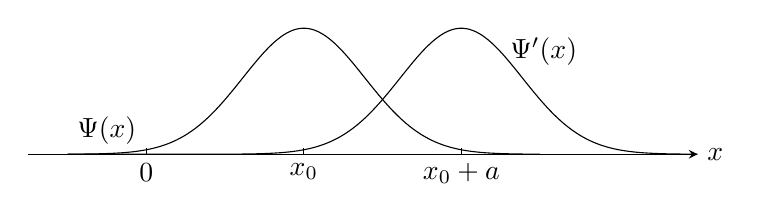
\begin{tikzpicture}[>=stealth]
        % assi
        \draw[->] (-0.5,0) -- (8,0) node[right] {$x$};
        % tacche e etichette
        \draw (1,0) -- (1,0.08) node[below,yshift=-2pt] {$0$};
        \draw (3,0) -- (3,0.08) node[below,yshift=-2pt] {$x_0$};
        \draw (5,0) -- (5,0.08) node[below,yshift=-2pt] {$x_0+a$};
        % profili d'onda (gaussiane stilizzate)
        \draw[smooth,domain=0:6,samples=200]
            plot(\x,{1.6*exp(-((\x-3)^2)/1.2)}) node[pos=0.28,above right] {$\Psi(x)$};
        \draw[smooth,domain=0:8,samples=200]
            plot(\x,{1.6*exp(-((\x-5)^2)/1.2)}) node[pos=0.78,above right , xshift = 5.5cm, yshift = 1cm] {$\Psi'(x)$};
    \end{tikzpicture}
    \caption{Traslazione di una funzione d'onda: $\Psi'(x)=\Psi(x-a)$.}
    \label{fig:traslazione-1d}
\end{figure}

L'operatore \(U(a)\) trasla la funzione d'onda, mentre l'operatore \(X'\) trasla il sistema di riferimento,
quindi i valori medi misurati sono gli stessi. 
Mentre l'operatore momento rimane invariato come ci si aspetta da una traslazione spaziale.

Per il teorema di Stone \ref{theo: Stone} deve esistere un generatore infinitesimo della trasformazione:
\[
    \bra{x} i\hbar\dv{a}U(a)\eval_{0}\ket{\Psi}= i\hbar \lim_{a\to 0 }   \frac{\bra{x}U(a)\ket{\Psi}-\braket{x}{\Psi}}{a}= i\hbar\lim_{a\to0 }\frac{\Psi(x-a)-\Psi(x)}{a} = -i\hbar \dv{x}\Psi(x)
\]
Che, in rappresentazione \(x\), corrisponde all'operatore momento \(P\) che dunque è il generatore infinitesimo di traslazioni:
\begin{equation}
    U(a) = e^{-\frac{i}{\hbar}aP}
\end{equation}


% Commutatore canonico e traslazioni generate da P
Supponiamo di partire da un sistema quantistico con
\[
    [Q,P]= i\hbar , \qquad Q,P \text{ a.a.}
\]
(coerente con la quantizzazione del corrispondente sistema classico).
Dato che \(P\) è a.a., l’operatore
\begin{equation}
    U(a)\equiv e^{-\frac{i}{\hbar}aP} \qquad a\in\mathbb{R}
\end{equation}
è un gruppo uniparametrico di operatori unitari.

\begin{equation}
    [Q,U(a)] =\left[ Q, e^{-\frac{i}{\hbar}aP} \right]     = aU(a)
\end{equation}


Sia \(\ket{q}\) un autovettore (generalizzato) di \(Q\): \(Q\ket{q}=q\ket{q}\): 
\[
    Q\,U(a)\ket{q}= \bigl(U(a)Q + aU(a)\bigr)\ket{q}
    = (q+a)\,U(a)\ket{q}
\]
Dunque \(U(a)\ket{q}\) è ancora autovettore di \(Q\) con autovalore \(q+a\).
Poiché \(a\in\mathbb{R}\) è arbitrario, segue che lo spettro di \(Q\) è traslato di qualsiasi quantità reale:
\[
    q\in\sigma(Q)\ \Longrightarrow\ q+a\in\sigma(Q)\ \ \forall\,a\in\mathbb{R}
    \quad\Longrightarrow\quad \sigma(Q)=\mathbb{R}
\]


Gli operatori \(U(a)=e^{-\frac{i}{\hbar}aP}\) realizzano le traslazioni di \(Q\);
equivalentemente, \(P\) è il generatore infinitesimo delle traslazioni della variabile coniugata a \(Q\).


\subsection{Traslazioni spaziali in 3D}

Sia \(\vec a=(a_x,a_y,a_z)\). Le traslazioni formano un gruppo abeliano a tre parametri:
\[
\tau(\vec a)\circ\tau(\vec b)=\tau(\vec a+\vec b)=\tau(\vec b)\circ \tau(\vec a)
\]
La rappresentazione unitaria \(U(\vec a)\) agisce su stati e osservabili come
\[
\ket{\Psi'}=U(\vec a)\ket{\Psi}, 
\qquad \Psi'(\vec x)=\Psi(\vec x-\vec a), 
\qquad U(\vec a)\,\vec X\,U(\vec a)^\dagger=\vec X-\vec a, 
\qquad U(\vec a)\,\vec P\,U(\vec a)^\dagger=\vec P .
\]

I generatori infinitesimi lungo gli assi sono \(P_x,P_y,P_z\) e, in generale,
\begin{equation}
    P_i \;=\; i\hbar\,\pdv{U(\vec a)}{a_i}\bigg|_{\vec a=0}\qquad i=x,y,z
\end{equation}
Per una traslazione nella direzione unitaria \(\hat n\):
\[
i\hbar\,\dv{s}U(s\hat n)\bigg|_{s=0}= \vec P\!\cdot\!\hat n
\]
e, dato un vettore arbitrario \(\vec a\),
\[
i\hbar\,\dv{s}U(s\vec a)\bigg|_{s=0}= \vec P\!\cdot\!\vec a
\]

Dal teorema di Stone segue dunque
\begin{equation}
    U(\vec a)=\exp\!\left(-\frac{i}{\hbar}\,\vec P\!\cdot\!\vec a\right)
\end{equation}
Poiché \([P_i,P_j]=0\) si può fattorizzare (l’ordine è irrilevante):
\[
U(\vec a)=e^{-\frac{i}{\hbar}P_x a_x}\,e^{-\frac{i}{\hbar}P_y a_y}\,e^{-\frac{i}{\hbar}P_z a_z}
\]

% 16 Lezione del 03/11/2025

\subsection{Rotazioni 3D}
\lezione{16}{03/11/2025}

Consideriamo la trasformazione di un vettore \(\vec{x} \in \mathbb{R}^3 \to \vec{x'}= R\vec{x}\), in cui consideriamo le matrici \(3\times3\) di rotazione \(R \) tali che \(R^\intercal R = I_3\) detto \textit{gruppo ortogonale} \(O(3)\).\\
Vale che \(\forall R \in O(3), \ \det R = \pm 1 \), tra queste consideriamo il \textit{gruppo speciale ortogonale}:
\begin{equation}
    SO(3)= \left\{ R \in O(3): \det R = +1 \right\}
\end{equation}
\(O(3)\) e \(SO(3)\) sono gruppi di Lie.

\begin{definition}
    \((G, \cdot )\) è \textit{gruppo di Lie} se \(G\) è varietà differenziabile e \(\cdot : G \times G \to G \) è differenziabile. 
\end{definition}

\begin{example}
    \(U(n)=\left\{ U \in \text{Mat}_{n\times n } : U^\dagger U = I \right\}\) detto \textit{gruppo unitario}.\\
    \(SU(n) = \left\{ U \in U(n ) : \det U = +1 \right\}\) detto \textit{gruppo unitario speciale}.
\end{example}


Consideriamo ora rotazioni infinitesime della forma \(R = I + s \delta R + O(s^2)\). Per la condizione \(R^\intercal R =I\) otteniamo:
\[
    I= (I+s \delta R^\intercal + \dots )(I+s \delta R+ \dots )= I + s(\delta R^\intercal+\delta R )
    \implies \delta R^\intercal=-\delta R 
\]
Cioè deve essere una matrice antisimmetrica. Una base per lo spazio delle matrici antisimmetriche, detto \textit{algebra di Lie} di \(SO(3)\) e indicata con \(so(3)\), è data da:
\[
    T_1=\begin{pmatrix}
        0 & 0 & 0\\
        0 & 0 & -1\\
        0 & 1 & 0
    \end{pmatrix},\qquad
    T_2=\begin{pmatrix}
        0 & 0 & 1\\
        0 & 0 & 0\\
        -1 & 0 & 0
    \end{pmatrix},\qquad
    T_3=\begin{pmatrix}
        0 & -1 & 0\\
        1 & 0 & 0\\
        0 & 0 & 0
    \end{pmatrix} .
\]
I loro elementi sono compattiamente scritti come
\[
    (T_k)_{ij} = -\,\epsilon_{kij} \qquad i,j,k=1,2,3
\]
con $\epsilon_{kij}$ simbolo di Levi\,–\,Civita. \\
Se definiamo 
\[
    \vec T=(T_1,T_2,T_3)\,, \quad \vec\omega=(\omega_1,\omega_2,\omega_3)
\]
abbiamo che 
ogni matrice \(R \in SO(3)\) è data da \(R = e^{\vec{\omega}\cdot \vec{T}}\equiv R(\omega)\) e indica la rotazione lungo l'asse \(\vec{\omega}\) di un angolo \(\abs{\vec{\omega}}\).


\begin{example}
    \[
        \vec{\omega}= \begin{pmatrix}
            0\\0\\\pi/3
        \end{pmatrix}\implies e^{\frac{\pi}{3}T_3} = \begin{pmatrix}
            \cos \frac{\pi}{3}& - \sin \frac{\pi}{3} & 0\\
            \sin \frac{\pi}{3} &\cos \frac{\pi}{3} & 0\\
            0&0&1
        \end{pmatrix}
    \]
\end{example}
\begin{remark}
    Vale la relazione: \(T_k = \pdv{R(\vec{\omega})}{\omega_k}\eval_{\vec{\omega}=0}\).
\end{remark}

\begin{remark}
    In genereale, \(e^{\vec{\omega}\cdot\vec{T}}e^{\vec{\omega'}\cdot\vec{T}} \neq e^{(\vec{\omega}+\vec{\omega'})\cdot\vec{T}}\) perché \(\left[ T_i, T_j \right]= \sum_k \epsilon_{ijk}T_k \neq 0\) .
\end{remark}

Vediamo ora sistemi quantistici con simmetria \(SO(3)\). A ogni \(R(\vec{\omega}) \in SO(3)\) per il teorema di Wigner \ref{theo: Wigner} deve essere associato un operatore unitario \(U_{R(\vec{\omega})}\equiv U(\vec{\omega})= e^{-\frac{i}{\hbar}\vec{\omega}\cdot\vec{J}}\).\\
Nella stessa maniera in cui \(SO(3)\) induce un algebra di Lie \(so(3)\), \(U_{R(\vec{\omega})}\) induce per il teorema di Stone \ref{theo: Stone} un insieme di operatori a.a.:
\begin{equation}
    \frac{1}{i\hbar} J_k := \pdv{U(\vec{\omega})}{\omega_k}\eval_{\vec{\omega}=0}
\end{equation}

Dunque se \(U(\vec{\omega})\) è rappresentazione unitaria non proiettiva di \(SO(3)\) e \(\frac{1}{i\hbar}J_k\) sono rappresentazione autoaggiunta di \(so(3)\) e dovranno avere le stesse relazioni di commutazione:
\begin{equation}
    \left[ J_i , J_k\right] = i\hbar\sum_k \epsilon_{ijk} J_k
\end{equation}
I \(J_k\) corrispondono alle componenti del momento angolare.

Se invece \(U(\vec{\omega})\) è rappresentazione genuinamente proiettiva, ottengo:
\[
    \left[ J_i , J_k\right] = i\hbar\sum_k \epsilon_{ijk} J_k + c_{ij} I 
\]
ma nel caso di \(so(3)\) si può sempre porre \(c_{ij}= 0 \ \forall\,i,j\) .\\
Inoltre, si ha il problema che per \(\vec{\omega}= (0 \ 0 \ \pi)\) avrò:
\[
    R(\vec{\omega })R(\vec{\omega}) = I  \quad  \text{ ma }\quad  U_{R(\vec{\omega}) }U_{R(\vec{\omega}) }= \pm I 
\]


\begin{example}
    \textbf{Particella in 3D senza spin}
    \[
        \mathcal{H} = L_2(\mathbb{R}) \quad R \in SO(3)\qquad
        \ket{\Psi' }= U(R)\ket{\Psi} \qquad \Psi'(\vec{x})= \Psi(R^{-1}\vec{x}) 
    \]
    \[
        U(R)\vec{X}U(R)^\dagger = R^{-1} \vec{X}    \qquad U(R)\vec{P}U(R)^\dagger = R^{-1}\vec{P}  
    \]
    Il generatore infinitesimo è dato da \(J_k = i\hbar  \pdv{U(\vec{\omega})}{\omega_k}\eval_{\vec{\omega}=0}\) 
    e vogliamo mostrare che in questo sistema: \(\vec{J}= \vec{L}:= \vec{X}\times \vec{P}\) con \( L_k = \sum_{i,j}\epsilon_{kij}X_i P_j\)

    \[
    \bra{\vec{x}}J_k\ket{\Psi}
    = i\hbar\,\pdv{}{\omega_k}\bra{\vec{x}}U(\vec{\omega})\ket{\Psi}\eval_{\vec{\omega}=0}
    = i\hbar\,\pdv{}{\omega_k}\Psi\!\big(R(\vec{\omega})^{-1}\vec{x}\big)\eval_{\vec{\omega}=0}
    \]

    \[
    = i\hbar\sum_{j=1}^{3}(\pdv{x_j}\Psi)\,\pdv{}{\omega_k}\!\left[(R(-\vec{\omega})\vec{x})_j\right]\eval_{\vec{\omega}=0}
    \]

    Sviluppando \(R(-\vec{\omega})=I-\sum_m\omega_mT_m+\dots\) con 
    \((T_m)_{j\ell}=-\epsilon_{m j \ell}\), si ha:
    \[
    (R(-\vec{\omega})\vec{x})_j = x_j - \sum_{k,\ell}\omega_k(T_k)_{j\ell}x_\ell+ \dots
    = x_j - \sum_{k,\ell}\omega_k\epsilon_{k \ell j}x_\ell + \dots
    \]

    \[
    \implies \pdv{}{\omega_k} \left(R(-\vec{\omega})\vec{x}\right)_j\eval_{\vec{\omega}=0}
    = \sum_{\ell}-\epsilon_{k  \ell j}x_\ell
    \]

    \[
    \implies \bra{\vec{x}}J_k\ket{\Psi}
    = i\hbar\sum_{j,\ell}-\epsilon_{k  \ell j}x_\ell(\pdv{j}\Psi)
    = \sum_{j,\ell}\epsilon_{k\ell j}x_\ell(-i\hbar\pdv{j})\Psi
    = \sum_{j,\ell}\epsilon_{k\ell j}X_\ell P_j\Psi
    \]

    \[
    \boxed{J_k = \sum_{j,\ell}\epsilon_{k\ell j}X_\ell P_j = L_k}
    \]
    Vale inoltre: \(\left[ L_i, L_j \right]= i\hbar \sum_k \epsilon_{ijk} L_k\)

    \begin{attention}
        \(\vec{L}\) è il momento angolare orbitale, \(\vec{J}\) è il momento angolare totale. In alcuni sistemi fisici \(\vec{J}\neq \vec{L}\).
    \end{attention}
\end{example}

\begin{definition}
    Se ho terna di operatori \(\vec{V}\equiv (V_1,V_2,V_3)\), si dice che la terna trasforma come un vettore per \(SO(3)\) se e solo se:
    \begin{equation}
        \left[ J_j, V_k  \right]= i\hbar \sum_{l}\epsilon_{jkl}V_l \iff U(\vec{\omega}) V_j U (\vec{\omega})^\dagger = \sum_{k} R(\vec{\omega})^{-1}_{jk}V_k
    \end{equation}
\end{definition}
\begin{definition}
    Diciamo che un operatore \(S\) è \textit{scalare} per rotazioni se vale:
    \begin{equation}
        \left[ J_i,S \right]=0 \quad i = 1,2,3 \qquad \ U(\vec{\omega})S U(\vec{\omega})^{\dagger} = S
    \end{equation}
\end{definition}
\begin{example}
    Se ho una terna che traforma come vettore ad esempio \(\vec{P}\), i loro moduli ad esempio \(P^2 = \vec{P}\cdot \vec{P}\) sono scalari.
\end{example}


% 17 Lezione del 04/10/2025

\subsubsection{Rototraslazioni}
\lezione{17}{04/10/2025}

Una rototraslazione è una trasformazione descritta da:
\begin{equation}
    g = (R, \vec{a})= (I, \vec{a})(R,0) \qquad \vec{x}'= (R, \vec{a})\vec{x}= R\vec{x}+ \vec{a}
\end{equation}
definita in modo che prima avvenga la rotazione e successivamente la traslazione.\\
Le rototraslazioni formano ovviamente un gruppo, la cui identità: \(id = (I,0)\), l'inversa è \((R,\vec{a})^{-1}= (R^{-1}, -R^{-1}\vec{a})\) e la composizione vale:
\[
(R_1,\vec{a_1})(R_2, \vec{a_2})\vec{x}= (R _1, \vec{a})(R_2\vec{x}+\vec{a_2})= R_1R_2\vec{x}+ R_1\vec{a}+ \vec{a_1}= (R_1R_2, R_1\vec{a_2}+\vec{a_1})
\]
Che verifica la definizione di inversa:
\[
    (R, \vec{a})(R^{-1}, R^{-1}\vec{a}) = (I, - RR^{-1}\vec{a}+\vec{a})= (I,0)
\]
Essendo una composizione di rotazioni e traslazioni la rappresentazione unitaria è data da:
\[
    U_{(R, \vec{a})}= U_{\vec{a}}U_{R(\vec{\omega})}= e^{-\frac{i}{\hbar}\vec{P}\cdot\vec{a}}e^{-\frac{i}{\hbar}\vec{\omega}\cdot\vec{j}}
\]
Abbiamo quindi un gruppo a 6 parametri generato da le \(J_i e P_i\), la cui algebra è data da:
\[
    \left[ J_i, J_j  \right]= i\hbar \sum_k\epsilon_{ijk}J_k \qquad 
    \left[ P_i, P_j \right] =0 \qquad \left[ J_i, P_j\right] = i\hbar \sum_k    \epsilon_{ijk}P_k
\]




\section{Simmetrie della dinamica}
Consideriamo \(\ket{\Psi(t)}\) soluzione equazione di Schrödinger e una simmetria \(\tau\) descritta da un operatore unitario e indipendente dal tempo \(W\).\\
\(\ket{\Psi'(t)}= W\ket{\Psi(t)} \ \forall\,t \) è ancora soluzione dell'eq di Schrödinger? 
\[
    i\hbar\dv{t}W\ket{\Psi(t)} =   W i\hbar \dv{t}\ket{\Psi(t)} = W H(t)\ket{\Psi(t)} \equiv H(t)W\ket{\Psi(t)}  \iff \left[ W, H(t) \right]=0
\]

\begin{definition}
    Definiamo il \textit{gruppo di simmetrie della dinamica} come:
    \begin{equation}
        G_d = \left\{ W \text{ (anti)unitari }  : \ \left[ W, H \right]=0 \right\} \subseteq G
    \end{equation}
    Questo è equivalente a \(WHW^\dagger= H\) e se \(W\) è unitario (non anti) allora \(\left[ W, U(t,t_0) \right]=0\)
\end{definition}

Nella visuale di Heisenberg, con \(A_h(t)= U(t-t_0)^\dagger A_s U(t-t_0)\)
se \(W \in G_d\) vale:
\[
    WA_h(t)W^\dagger = U(t-t_0)^\dagger W A_s W^\dagger U(t-t_0)
\]
è ancora soluzione dell'eq di Heisenberg.

Se \(W\) formano un gruppo a un parametro \(W(s)= e^{-\frac{i}{\hbar}sQ}\) vale:
\begin{equation}
    \left[ W(s), H \right]= 0 \ \forall\, s \iff \left[ Q, H \right]    =0 \iff \dv{t} \expval{Q}_\Psi (t)=0 \quad \forall\, \Psi \in \mathcal{H}
\end{equation}
Esiste relazione diretta tra simmetrie di un sistema e quantità conservate.

\begin{theorem}\label{theo: Noether}
    {\normalfont\textbf{di Noether in MQ}}\\
    \(H\) è invariante per simmetria generata da operatore \(Q\) autoaggiunto se e solo se \(Q\) è quantità conservata.
\end{theorem}

\begin{remark}
    Dato \(W\) unitario, \(\left[ W, H \right]=0\) e \(H\ket{E}= E\ket{E}\), allora:
    \begin{equation}
        HW\ket{E} = WH\ket{E}= EW\ket{E}
    \end{equation}
    \(W\ket{E}\) è ancora autovettore di \(H\) con stesso autovalore.
\end{remark}

\begin{remark}
    Se esistono due autovettori \(\ket{E,1}\) e \(\ket{E,2}\) degeneri di \(H\), tali che \(\braket{E,r}{E,s}= \delta_{rs}\),
    allora esite operatore unitario \(W\) tale che:
    \begin{equation}
        \left[ W, H \right]= 0 \quad \begin{cases}
                W\ket{E,1}= \ket{E,2}\\ W\ket{E,2}=\ket{E,1}
            \end{cases}
    \end{equation}
\end{remark}
\begin{proof}
    Data \(\left\{ \ket{E,1}\equiv \ket{1}, \ket{E,2}\equiv \ket{2}, \ket{3},\ket{4}, \dots  \right\}\) base ON di autovettori di \(H\), definisco mappa lineare \(W\) tale che:
    \[
        W\ket{E,1}= \ket{E,2} \quad  W\ket{E,2}=\ket{E,1} \qquad W\ket{n}= \ket{n} \quad n\geq 3
    \]
    è unitario perché mappa base ON in base ON e vale \((WH-HW)\ket{n}=0 \quad \forall,n\)
\end{proof}

Di consueguenza sappiamo che se \(\sigma(H)\) è completamente non degenere \(\left\{ \ket{E} \right\}_{E \in \sigma(H)}\) e \(W \) unitario \(\left[ W, H \right]=0\), 
allora per la prima osservazione abbiamo che \(W\ket{E}= f(E)\ket{E}\) con \(f(E)\in \mathbb{C} \quad \forall, E \in \sigma(H)\), dunque \(W = f(H)\). 
Chiamiamo tali operatori \textit{gruppo di simmetrie banali della dinamica}:
\begin{equation}
    K_d:= \left\{ W \text{ unitari } : \ W = f(H) \right\}   \subseteq G_d
\end{equation}
Perciò se \(\sigma(H)\) è completamente non degenere, \(K_d= G_d\)  e tutte le simmetrie delle dinamica possibili sono banali.\\
Se invece \(E \in \sigma(H)\) è degenere, per la seconda osservazione esiste un \(W \in G_d, \ W \notin K_d\), cioè ammette simmetrie non banali.


\subsection{Traslazioni temporali}
L'omogeneità nel tempo per sistemi conservativi induce una simmetria per traslazioni temporali, data da un gruppo ad un parametro \(U(t)= e^{-\frac{i}{\hbar}Ht}\) che trasforma:
\[
    \ket{\Psi'}= U(t)\ket{\Psi} \qquad A'=U(t)AU(t)^\dagger 
\]
\begin{attention}
    Non si tratta di evoluzione causale, stiamo cambiando sia le funzione d'onda che gli operatori e le medie rimangono invariate. 
    Invece, nell'evoluzione casuale, cambiano solo le funzioni d'onda nella visuale di Schrödinger o solo gli operatori in quella di Heisenberg.
\end{attention}


\section{Simmetrie discrete}
\subsection{Parità Spaziale}
Consideriamo ora la riflessione rispetto all'origine: \(\vec{x}\to -\vec{x}\) descritta dalla matrice:
\[
    R_p = \begin{pmatrix}
        -1&0&0\\0&-1&0\\0&0&-1
    \end{pmatrix}
    \in O(3) \quad \notin SO(3) \ (\det = -1)
\]
Notiamo che tutte le \textit{rotazioni impoprie} cioè \(\forall\, g \in O(3) \ \notin SO(3)\) possono essere scritte come \(g = R_pR(\vec{\omega})\) con \(R(\vec{\omega})\in SO(3)\).

Consideriamo una particella senza spin in 3D e un operatore \(\mathbb{P}\) che agisce come:
\[
    \mathbb{P}\vec{X}\mathbb{P}^\dagger = -\vec{X} \qquad \mathbb{P}\vec{P}\mathbb{P}^\dagger = -\vec{P} \qquad \mathbb{P}\vec{L}\mathbb{P}^\dagger = \vec{L}  
\]
Gli operatori \(\vec{X}\) e \(\vec{P}\) per questo si dicono \textit{vettori polari} e \(\vec{L}\) si dice \textit{vettore assiale}.


Verifichiamo se \(\mathbb{P}\) è unitario o antiunitario:
\begin{equation*}
\left[ \, \mathbb{P} X_j \mathbb{P}^\dagger ,\, \mathbb{P} P_k \mathbb{P}^\dagger \right]
= \mathbb{P}\,[X_j,P_k] \,\mathbb{P}^\dagger
= \mathbb{P}\,(i\hbar\,\delta_{jk})\,\mathbb{P}^\dagger 
= \begin{cases}
 i\hbar\,\delta_{jk}, & \mathbb{P} \text{ unitario},\\
 -i\hbar\,\delta_{jk}, & \mathbb{P} \text{ antiunitario}.
 \end{cases}
\end{equation*}

Dalla definizione di \(\mathbb{P}\) otteniamo:
\[
\left[ \, \mathbb{P} X_j \mathbb{P}^\dagger ,\, \mathbb{P} P_k \mathbb{P}^\dagger \right]
= [-X_j,-P_k] = i\hbar\,\delta_{jk}.
\]
Confrontando i due risultati segue che \(\mathbb{P}\) è unitario.

Dato che \(\mathbb{P}^2 = I\) segue che \(\mathbb{P}= \mathbb{P}^{-1}= \mathbb{P}^\dagger\) cioé è sia unitario che autoaggiunto.\\
Lo spettro \(\sigma(\mathbb{P})= \left\{ \pm 1   \right\}\), dunque per autovalore \(n_p \in \sigma(\mathbb{P})\) vale:
\[
    \bra{\vec{x}}\mathbb{P}\ket{\Psi}= n_p\braket{\vec{x}}{\Psi} \iff \Psi(-\vec{x}) = n_p \Psi(\vec{x})
\]
dunque gli autostati di \(n_p=1\) sono le funzioni d'onda pari, per \(n_p= -1\) le funzioni d'onda dispari.

Per l'operatore hamiltoniano:
\[
    H = \frac{\abs{\vec{P}}^2}{2m} + V(\vec{x}) \to \mathbb{P}H\mathbb{P}= \frac{\abs{\vec{P}}^2}{2m} + V(-\vec{x}) 
\]
Perciò se \(V(\vec{x})= V(-\vec{x})\) allora \(\mathbb{P} \in G_d\).



% 18 Lezione del 07/11/2025

\subsection{Inversione temporale}
\lezione{18}{07/11/2025}

Consideriamo l'operatore \(\mathbb{T}\) che agisca nella seguente maniera:
\[
    \vec{x}\to \vec{x} \quad t \to -t \qquad \mathbb{T}\vec{X}\mathbb{T}^\dagger = \vec{X} \qquad  \mathbb{T}\vec{P}\mathbb{T}^\dagger = - \vec{P} \qquad  \mathbb{T}\vec{L}\mathbb{T}^\dagger = - \vec{L}
\]

In questo caso:
\begin{align*}
    \left[ \mathbb{T}X_j\mathbb{T}^\dagger,\mathbb{T}P_k\mathbb{T}^\dagger \right] 
    &= \mathbb{T}\left[ X_j, P_k \right]\mathbb{T}^\dagger = \mathbb{T}i \hbar \delta_{jk}\mathbb{T}^\dagger \\
    &= - \left[ X_j, P_k \right] = -i\hbar \delta_{jk}
\end{align*}
Dunque \(\mathbb{T}\) è antiunitario, perciò \(\braket{\chi}{\mathbb{T}\Psi}= \overline{\braket{\mathbb{T}\chi}{\Psi}}\).
Come agisce \(\mathbb{T}\) sullo stato \(\ket{\Psi}\) ?
\[
    \mathbb{T}\ket{\Psi}= \mathbb{T}\int_{\mathbb{R}^3}\dd[3]{x}\ket{\vec{x}}\braket{\vec{x}}{\Psi} = \int_{\mathbb{R}^3}\dd[3]{x}\ket{\vec{x}}\braket{\vec{x}}{\Psi}^*
    \implies \Psi'(\vec{x})= \Psi(\vec{x})^*
\]
Un sistema è invariante per inversione temporale se l'Hamiltoniana \(H\) commuta con \(\mathbb{T}\).
\[
    [\mathbb{T}, H] = 0 \iff H = \mathbb{T} H \mathbb{T}^\dagger
\]
Per un sistema conservativo, l'operatore di evoluzione temporale \(U(t) = e^{-\frac{i}{\hbar}Ht}\) si trasforma come:
\begin{equation}
    \mathbb{T} U(t) \mathbb{T}^\dagger = \mathbb{T} e^{-\frac{i}{\hbar}Ht} \mathbb{T}^\dagger = e^{\frac{i}{\hbar}Ht} = U(-t)
\end{equation}
Data una soluzione dell'equazione di Schrödinger \(\ket{\Psi(t)} = U(t)\ket{\Psi(0)}\), lo stato trasformato \(\mathbb{T}\ket{\Psi(t)}\) evolve come:
\[
    \mathbb{T}\ket{\Psi(t)} = \mathbb{T} U(t) \mathbb{T}^\dagger \mathbb{T}\ket{\Psi(0)} = U(-t) \mathbb{T}\ket{\Psi(0)}
\]
Questo stato \textbf{non è una soluzione} dell'equazione di Schrödinger, poiché la sua evoluzione temporale è invertita rispetto a quella richiesta.

Tuttavia, se definiamo un nuovo stato \(\ket{\Psi'(t)}\) come lo stato originale evoluto all'indietro nel tempo e poi trasformato con \(\mathbb{T}\):
\[
    \ket{\Psi'(t)} := \mathbb{T}\ket{\Psi(-t)}
\]
allora \(\ket{\Psi'(t)}\) \textbf{è una soluzione} dell'equazione di Schrödinger.
Infatti:
\[
    \ket{\Psi'(t)} = \mathbb{T} U(-t) \ket{\Psi(0)} = \left( \mathbb{T} U(-t) \mathbb{T}^\dagger \right) \mathbb{T}\ket{\Psi(0)} = U(t) \mathbb{T}\ket{\Psi(0)}
\]
Lo stato \(\ket{\Psi'(t)}\) evolve correttamente a partire da un nuovo stato iniziale \(\ket{\Psi'(0)} = \mathbb{T}\ket{\Psi(0)}\).

Nella rappresentazione delle coordinate, questo significa che se \(\Psi(\vec{x}, t)\) è una soluzione, allora lo è anche la sua complessa coniugata con il tempo invertito.
\[
    \braket{\vec{x}}{\Psi'(t)} = \braket{\vec{x}}{\mathbb{T} | \Psi(-t)} = \braket{\vec{x}}{\Psi(-t)}^* = \Psi^*(\vec{x}, -t)
\]

Se \(\Psi(\vec{x}, t)\) è soluzione all'equazione di Schrödinger per un sistema con simmetria di inversione temporale, allora lo è anche \(\Psi^*(\vec{x}, -t)\).



\subsection{Spettro del momento angolare}
Consideriamo un sistema quantistico con simmetria di rotazione \(SO(3)\).
Il momento angolare totale \(\vec{J} = (J_x, J_y, J_z)\) è un insieme di operatori autoaggiunti che generano le rotazioni tramite \(U(\vec{\alpha}) = e^{-\frac{i}{\hbar}\vec{\alpha} \cdot \vec{J}}\)
e obbediscono all'algebra di Lie di \(so(3)\):
\begin{equation}
    [J_i, J_j] = i\hbar \sum_k \epsilon_{ijk} J_k
\end{equation}
Per studiare lo spettro, ci concentriamo su \(J_z\), ma i risultati si estendono a \(J_x\) e \(J_y\) per simmetria.
\begin{remark}
    Gli spettri delle componenti del momento angolare coincidono, \(\sigma(J_z) = \sigma(J_x) = \sigma(J_y)\),
    poiché le componenti sono collegate da trasformazioni unitarie (rotazioni).
\end{remark}

Definiamo l'operatore \(\vec{J}^2 = J_x^2 + J_y^2 + J_z^2\), che è uno scalare rotazionale e quindi commuta con tutte le componenti di \(\vec{J}\):
\[
    [\vec{J}^2, J_k] = 0
\]
Per trovare lo spettro di \(J_z\), introduciamo gli \textit{operatori di innalzamento e abbassamento} (o operatori scala):
\begin{equation}
    J_\pm := J_x \pm i J_y.
\end{equation}
Valgono le seguenti proprietà:
\[
    (J_\pm)^\dagger = J_\mp, \qquad \left[ \vec{J}^2, J_\pm \right] = 0, \qquad J_x = \frac{J_+ + J_-}{2}, \qquad J_y = \frac{J_+ - J_-}{2i}.
\]
Inoltre, valgono le relazioni di commutazione:
\[
    [J_z, J_\pm] = [J_z, J_x] \pm i[J_z, J_y]
    = (i\hbar J_y) \pm i(-i\hbar J_x) = \pm \hbar (J_x \pm i J_y) = \pm \hbar J_\pm.
\]
I prodotti \(J_+ J_-\) e \(J_- J_+\) si possono esprimere in termini di \(\vec{J}^2\) e \(J_z\):
\[
    J_+ J_- = (J_x + i J_y)(J_x - i J_y) = J_x^2 + J_y^2 - i[J_x, J_y] = J_x^2 + J_y^2 + \hbar J_z = \vec{J}^2 - J_z^2 + \hbar J_z,
\]
\[
    J_- J_+ = (J_x - i J_y)(J_x + i J_y) = J_x^2 + J_y^2 + i[J_x, J_y] = J_x^2 + J_y^2 - \hbar J_z = \vec{J}^2 - J_z^2 - \hbar J_z.
\]
Da cui si ricava il commutatore:
\[
    [J_+, J_-] = 2\hbar J_z.
\]

L'operatore \(\vec{J}^2\) è semidefinito positivo. Infatti, per ogni stato \(\ket{\Psi}\):
\[
    \expval{\vec{J}^2}_\Psi = \bra{\Psi} (J_x^2 + J_y^2 + J_z^2) \ket{\Psi}
    = \norm{J_x \ket{\Psi}}^2 + \norm{J_y \ket{\Psi}}^2 + \norm{J_z \ket{\Psi}}^2 \ge 0.
\]
Di conseguenza, il suo spettro è non negativo: \(\sigma(\vec{J}^2) \subseteq \mathbb{R}_{\ge 0}\).

Poiché \([\vec{J}^2, J_z]=0\), possiamo trovare una base ortonormale di autostati comuni \(\left\{ \ket{j, m} \right\}\).
Definiamo i loro autovalori:
\begin{align}
    \vec{J}^2 \ket{j, m} &= \hbar^2 j(j+1) \ket{j, m}, \quad j \ge 0 \\
    J_z \ket{j, m} &= \hbar m \ket{j, m}, \quad m \in \mathbb{R}
\end{align}
La parametrizzazione dell'autovalore di \(\vec{J}^2\) come \(\hbar^2 j(j+1)\) è una scelta standard che si rivelerà conveniente. La condizione \(\vec{J}^2 \ge 0\) è soddisfatta per \(j \ge 0\).

Applichiamo ora gli operatori scala \(J_\pm\) agli autostati \(\ket{j,m}\). Poiché \([\vec{J}^2, J_\pm]=0\), il valore di \(j\) non cambia:
\[
    \vec{J}^2 (J_\pm \ket{j, m}) = J_\pm \vec{J}^2 \ket{j, m} = \hbar^2 j(j+1) (J_\pm \ket{j, m}).
\]
Invece, l'autovalore di \(J_z\) viene traslato:
\[
    J_z (J_\pm \ket{j, m}) = (J_\pm J_z + [J_z, J_\pm]) \ket{j, m}
    = (J_\pm \hbar m \pm \hbar J_\pm) \ket{j, m}
    = \hbar (m \pm 1) (J_\pm \ket{j, m}).
\]
Lo stato \(J_\pm \ket{j, m}\) è quindi un autostato di \(J_z\) con autovalore \(\hbar(m\pm 1)\).

Perché \(J_\pm \ket{j, m}\) sia un autostato valido, non deve essere il vettore nullo. Calcoliamone la norma (assumendo \(\braket{j, m}{j, m} = 1\)):
\[
    \norm{J_\pm \ket{j, m}}^2 = \bra{j, m} J_\mp J_\pm \ket{j, m}
    = \bra{j, m} (\vec{J}^2 - J_z^2 \mp \hbar J_z) \ket{j, m}
\]
Sostituendo gli autovalori, otteniamo:
\[
    \norm{J_\pm \ket{j, m}}^2 = \hbar^2 [j(j+1) - m^2 \mp m]
    = \hbar^2 [j(j+1) - m(m \pm 1)]
\]
Poiché la norma quadra deve essere non negativa, abbiamo due condizioni:
\begin{align*}
    \norm{J_+ \ket{j,m}}^2 \ge 0 \implies j(j+1) - m(m+1) \ge 0 \\
    \norm{J_- \ket{j,m}}^2 \ge 0 \implies j(j+1) - m(m-1) \ge 0
\end{align*}
Queste due disequazioni sono entrambe soddisfatte se e solo se:
\begin{equation}
    -j \le m \le j.
\end{equation}
Per un dato \(j\), i valori di \(m\) sono quindi limitati.

La sequenza di autostati \(\dots, \ket{j, m-1}, \ket{j, m}, \ket{j, m+1}, \dots\) deve essere finita.
Ciò accade quando il vettore diventa nullo:
\begin{itemize}
    \item Deve esistere un \(m_\text{max}\) tale che \(J_+ \ket{j, m_\text{max}} = 0\).
    Dalla condizione sulla norma, \(j(j+1) - m_\text{max}(m_\text{max}+1) = 0\), che implica \(m_\text{max} = j\).
    \item Deve esistere un \(m_\text{min}\) tale che \(J_- \ket{j, m_\text{min}} = 0\).
    Similmente, \(j(j+1) - m_\text{min}(m_\text{min}-1) = 0\), che implica \(m_\text{min} = -j\).
\end{itemize}
Partendo da \(m_\text{min} = -j\), si deve poter raggiungere \(m_\text{max} = j\) con un numero intero \(k\) di passi da \(+1\) (applicando \(J_+\) ripetutamente):
\[
    m_\text{max} - m_\text{min} = k, \quad k \in \mathbb{Z}_{\ge 0}
\]
\[
    j - (-j) = k \implies 2j = k.
\]
Questo implica che \(2j\) deve essere un numero intero non negativo. I valori possibili per \(j\) sono quindi:
\[
    j = 0, \frac{1}{2}, 1, \frac{3}{2}, \dots
\]
Per un dato \(j\), i valori permessi di \(m\) sono \(2j+1\) valori equispaziati:
\[
    m = -j, -j+1, \dots, j-1, j.
\]




% 19 Lezione del 10/11/2025
\lezione{19}{10/11/2025}
Consideriamo una base ON di autostati \(\left\{ \ket{j,m} \right\} \)  per un certo \( j\) fissato con \(m \in \{-j, \dots, j\}\).

Partendo dall'autostato dell'autovalore più grande \(m=j\,, \ \  \norm{\ket{j,j}}^2 = 1\), posso ottenere gli altri elementi della base grazie all'operatore di abbassamento:
\[
    \ket{j, m-1} := \frac{J_- \ket{j,m}}{\hbar \sqrt{j(j+1) - m(m-1)}} \quad \text{per } m > -j
\]
Che viene opportunamente normalizzato. Alla stessa maniera l'operatore di innalzamento agisce come:
\[
    J_+ \ket{j,m} = \frac{J_+ J_- \ket{j,m+1}}{\hbar \sqrt{j(j+1) - m(m+1)}} = \hbar \sqrt{j(j+1)-(m+1)m} \ket{j, m+1}
\]

Quindi gli operatori di innalzamento e abbassamento, aumentano e diminuiscono rispettivamente l'autovalore \(m \) e aggiungono un fattore di proporzione dipendente da \(j\) e \(m\):
\begin{equation}
    J_\pm \ket{j,m} = \hbar \sqrt{j(j+1)-m(m\pm 1)} \ket{j, m \pm 1}
\end{equation}

Rispetto a questa base ortonormale \(\left\{ \ket{j,m} \right\}_{m=-j}^j\) (con \(j\) fissato), le rappresentazioni matriciali degli operatori del momento angolare hanno una forma conveniente:
\begin{itemize}
    \item Per \(J_z\), la rappresentazione è diagonale:
    \[
        \matrixel{j,m'}{J_z}{j,m} = m\hbar\,\delta_{m'm}
        \implies
        J_z = \hbar \begin{pmatrix} j & & & 0 \\ & j-1 & & \\ & & \ddots & \\ 0 & & & -j \end{pmatrix}.
    \]
    \item Per gli operatori scala \(J_\pm\), definendo per brevità $\mu_\pm(j,m) = \hbar \sqrt{j(j+1)-m(m\pm 1)}$, si ha:
    \[
        \matrixel{j,m'}{J_+}{j,m} = \mu_+(j,m)\,\delta_{m',m+1},
        \qquad
        \matrixel{j,m'}{J_-}{j,m} = \mu_-(j,m)\,\delta_{m',m-1}.
    \]
    Le matrici corrispondenti sono strettamente triangolari, con elementi non nulli solo sulla prima sovradiagonale per \(J_+\) e sulla prima sottodiagonale per \(J_-\).
    \[
        J_+ = \begin{pmatrix} 0 & \mu_+(j,j-1) & 0 & \dots \\ 0 & 0 & \mu_+(j,j-2) & \dots \\ \vdots & & \ddots & \mu_+(j,-j) \\ 0 & \dots & \dots & 0 \end{pmatrix},
    \]
    \[
        J_- = \begin{pmatrix} 0 & 0 & \dots & 0 \\ \mu_-(j,j) & 0 & \dots & 0 \\ 0 & \mu_-(j,j-1) & \ddots & \vdots \\ \vdots & & \ddots & 0 \\ 0 & \dots & \mu_-(j,-j+1) & 0 \end{pmatrix}.
    \]
    \item Per \(J_x\) e \(J_y\), le matrici si ottengono dalle relazioni \(J_x = (J_+ + J_-)/2\) e \(J_y = (J_+ - J_-)/(2i)\).
    Sono matrici tridiagonali con elementi nulli sulla diagonale principale.
    \[
        J_x = \frac{1}{2} \begin{pmatrix} 0 & \mu_+(j,j-1) & & 0 \\ \mu_-(j,j) & 0 & \mu_+(j,j-2) & \\ & \mu_-(j,j-1) & \ddots & \mu_+(j,-j) \\ 0 & & \mu_-(j,-j+1) & 0 \end{pmatrix},
    \]
    \[
        J_y = \frac{1}{2i} \begin{pmatrix} 0 & \mu_+(j,j-1) & & 0 \\ -\mu_-(j,j) & 0 & \mu_+(j,j-2) & \\ & -\mu_-(j,j-1) & \ddots & \mu_+(j,-j) \\ 0 & & -\mu_-(j,-j+1) & 0 \end{pmatrix}.
    \]
\end{itemize}


\subsubsection{Spettro degenere}

Se è presente degenerazione, l'autospazio \(\mathcal{H}_{j,m}\) associato agli autovalori \(j(j+1)\hbar^2\) e \(m\hbar\) ha dimensione \(d(j,m) > 1\).
Si considera una base ortonormale di questo autospazio, indicizzata da un numero quantico aggiuntivo $r$:
\[
    \{ \ket{j, m, r} \}_{r=1, \dots, d(j,m)}
\]
tale che $\braket{j, m, r}{j, m, r'} = \delta_{rr'}$.

Analizziamo l'azione degli operatori di scala, che agiscono sull'indice $m$ ma non sull'indice di degenerazione $r$.
Per \(m > -j\), l'operatore di abbassamento \(J_-\) mappa lo stato \(\ket{j, m, r}\) in un nuovo stato. Definiamo i vettori normalizzati:
\[
    \ket{j, m-1, r} := \frac{J_- \ket{j, m, r}}{\hbar \sqrt{j(j+1) - m(m-1)}}
\]
Questi vettori sono ortonormali rispetto all'indice $r$:
\[
    \braket{j, m-1, r}{j, m-1, r'} = \delta_{rr'}
\]
Poiché abbiamo costruito un sistema ortonormale di \(d(j,m)\) vettori nell'autospazio \(\mathcal{H}_{j, m-1}\), la sua dimensione deve essere almeno \(d(j,m)\):
\[
    d(j, m-1) \ge d(j, m)
\]

Allo stesso modo, per \(m < j\), l'operatore di innalzamento \(J_+\) permette di definire i vettori normalizzati:
\[
    \ket{j, m+1, r} := \frac{J_+ \ket{j, m, r}}{\hbar \sqrt{j(j+1) - m(m+1)}}
\]
Anche questi vettori sono ortonormali, $\braket{j, m+1, r}{j, m+1, r'} = \delta_{rr'}$, il che implica:
\[
    d(j, m+1) \ge d(j, m)
\]

Combinando i due risultati, \(d(j, m+1) \ge d(j, m)\) e \(d(j, m) \ge d(j, m-1)\), e applicando il ragionamento a catena per tutti i valori di \(m\) da \(-j\) a \(j\), si conclude che la degenerazione deve essere la stessa per tutti i livelli:
\[
    d(j, m) \text{ è indipendente da } m.
\]
Possiamo quindi indicarla semplicemente con \(d(j)\).

Gli operatori di scala definiscono isomorfismi tra gli autospazi adiacenti (eccetto ai bordi \(m=\pm j\)):
\[
    \mathcal{H}_{j, m-1} \xleftarrow{J_-} \mathcal{H}_{j,m} \xrightarrow{J_+} \mathcal{H}_{j, m+1}
\]
Tutti gli autospazi \(\mathcal{H}_{j,m}\) (per \(m \in \{-j, \dots, j\}\)) sono quindi isomorfi e hanno la stessa dimensione \(d(j)\).
Si può costruire l'intera base partendo da una base ortonormale \(\left\{ \ket{j, j, r} \right\}_{r=1, \dots, d(j)}\) dell'autospazio con \(m=j\) e applicando ricorsivamente l'operatore di abbassamento \(J_-\):
\[
    \ket{j, m-1, r} := \frac{J_- \ket{j, m, r}}{\hbar \sqrt{j(j+1) - m(m-1)}}
\]
La base completa per un dato valore di \(j\) è quindi:
\[
    \{ \ket{j, m, r} \}_{m \in \{-j, \dots, j\}, \, r=1, \dots, d(j)}
\]
I valori permessi per \(j\) e la loro degenerazione \(d(j)\) dipendono dalle specifiche simmetrie del sistema fisico in esame.

Invece di decomporre lo spazio di Hilbert totale \(\mathcal{H}\) negli autospazi \(\mathcal{H}_{j,m}\) (comuni a \(\vec{J}^2\) e \(J_z\)), è più conveniente utilizzare una decomposizione basata sugli indici \(j\) e sull'indice di degenerazione \(r\).

Fissiamo \(j\) e \(r\), con \(1 \le r \le d(j)\). Definiamo il sottospazio \(\mathcal{H}_{j,r}\) come lo spazio generato dalla base:
\[
    \{ \ket{j, m, r} \}_{m \in \{-j, \dots, j\}}
\]
La dimensione di questo spazio è \(\dim \mathcal{H}_{j,r} = 2j+1 < +\infty\).

Questi sottospazi \(\mathcal{H}_{j,r}\) sono \textbf{invarianti} (o stabili) sotto l'azione di tutti gli operatori del momento angolare \(\vec{J} = (J_x, J_y, J_z)\).
Gli operatori \(J_z\) e \(J_\pm\) agiscono solo sui vettori con lo stesso indice \(j\) e \(r\):
\begin{align*}
    J_z \ket{j, m, r} &= m\hbar \ket{j, m, r} \in \mathcal{H}_{j,r} \\
    J_\pm \ket{j, m, r} &= \hbar \sqrt{j(j+1) - m(m\pm 1)} \ket{j, m\pm 1, r} \in \mathcal{H}_{j,r}
\end{align*}
Di conseguenza, per qualsiasi stato \(\ket{\Psi} \in \mathcal{H}_{j,r}\), anche la sua trasformazione rimane nel sottospazio:
\[
    J_k \ket{\Psi} \in \mathcal{H}_{j,r} \quad (\text{per } k=x,y,z)
\]
e, più in generale, un operatore di rotazione finita lascia lo stato all'interno del sottospazio:
\[
    e^{-\frac{i}{\hbar} \vec{J} \cdot \vec{\omega}} \ket{\Psi} \in \mathcal{H}_{j,r}
\]

Lo spazio di Hilbert totale \(\mathcal{H}\) può quindi essere decomposto nella somma diretta di questi sottospazi invarianti:
\[
    \mathcal{H} = \bigoplus_j \bigoplus_{r=1}^{d(j)} \mathcal{H}_{j,r}
\]
Rispetto a questa decomposizione, la rappresentazione matriciale degli operatori del momento angolare (e delle rotazioni) diventa \textbf{diagonale a blocchi}. 
\[
e^{-\frac{i}{\hbar} \vec{J} \cdot \vec{\omega}} =
\begin{pmatrix}
    \begin{array}{|c|}
    \hline
    \text{Blocco } \mathcal{H}_{j,r} \\
    \hline
    \end{array}
    & 0 & \cdots \\
    0 &
    \begin{array}{|c|}
    \hline
    \text{Blocco } \mathcal{H}_{j',r'} \\
    \hline
    \end{array}
    & \cdots \\
    \vdots & \vdots & \ddots
\end{pmatrix}
\]
Ogni blocco, associato a un sottospazio \(\mathcal{H}_{j,r}\), è una matrice \((2j+1) \times (2j+1)\) che agisce solo sugli stati di quel sottospazio.

All'interno di un singolo blocco (fissando \(j\) e \(r\) e usando la base \(\{\ket{j,m,r}\}_{m=-j}^j\)):
\begin{itemize}
    \item \(J_z\) è rappresentato da una matrice diagonale.
    \item \(J_+\) e \(J_-\) sono rappresentati da matrici strettamente sopra/sotto-diagonali.
    \item \(J_x\), \(J_y\) e l'operatore di rotazione \(e^{-\frac{i}{\hbar} \vec{J} \cdot \vec{\omega}}\) sono rappresentati da matrici non diagonali.
\end{itemize}
Questa struttura a blocchi è fondamentale perché permette di studiare le proprietà di rotazione del sistema analizzando separatamente le rappresentazioni irriducibili del gruppo delle rotazioni, ciascuna corrispondente a un valore di \(j\).

\subsection{Particella senza spin in 3D}
\label{sec: particella3d}


Consideriamo una particella senza spin in 3 dimensioni, il cui spazio di Hilbert è \( \mathcal{H} = L_2(\mathbb{R}^3, \dd[3]{x}) \).
Le rotazioni sono implementate dall'operatore unitario \( U(R) \), che agisce sulla funzione d'onda come:
\begin{equation}
    (U(R)\Psi)(\vec{x}) = \Psi(R^{-1}\vec{x}).
\end{equation}
Gli operatori posizione e momento sono:
\begin{equation}
    \vec{X}\Psi(\vec{x}) = \vec{x}\Psi(\vec{x}), \qquad \vec{P}\Psi(\vec{x}) = -i\hbar\vec{\nabla}\Psi(\vec{x}).
\end{equation}
Per una particella senza spin, il momento angolare totale \( \vec{J} \) coincide con il momento angolare orbitale \( \vec{L} = \vec{X} \times \vec{P} \):
\begin{equation}
    \vec{J} \equiv \vec{L} = \vec{X} \times \vec{P} = -i\hbar (\vec{x} \times \vec{\nabla}).
\end{equation}
Vogliamo trovare le autofunzioni simultanee di \( L^2 \) e \( L_z \).
Le autofunzioni \( \Psi_{\ell,m}(\vec{x}) = \braket{\vec{x}}{\ell,m} \) devono soddisfare le equazioni agli autovalori:
\begin{align}
    L^2 \Psi_{\ell,m}(\vec{x}) &= \hbar^2 \ell(\ell+1) \Psi_{\ell,m}(\vec{x}) \\
    L_z \Psi_{\ell,m}(\vec{x}) &= \hbar m \Psi_{\ell,m}(\vec{x})
\end{align}

Per risolvere queste equazioni differenziali, è conveniente passare alle coordinate sferiche \( (r, \vartheta, \varphi) \).
Le relazioni tra coordinate cartesiane e sferiche sono:
\[
\begin{cases}
    x = r \sin\vartheta \cos\varphi \\
    y = r \sin\vartheta \sin\varphi \\
    z = r \cos\vartheta
\end{cases},
\qquad
\begin{cases}
    r = \sqrt{x^2+y^2+z^2} \in [0, \infty) \\
    \tan(\varphi) = \frac{y}{x} \quad \varphi \in [0, 2\pi] \\
    \cos(\vartheta) = \frac{z}{r} \quad \vartheta \in [0, \pi] 
\end{cases}
\]

La funzione d'onda si trasforma come \( \Psi(x,y,z) \rightsquigarrow \Psi(r, \vartheta, \varphi) \).
L'elemento di volume in coordinate sferiche è \( \dd[3]{x} = r^2 \sin\vartheta \, \dd{r} \dd{\vartheta} \dd{\varphi} \).
Di conseguenza, il prodotto scalare nello spazio di Hilbert \( \mathcal{H} = L_2(\mathbb{R}^3, r^2 \sin\vartheta \, \dd{r} \dd{\vartheta} \dd{\varphi}) \) diventa:
\begin{equation}
    \braket{\Psi_1}{\Psi_2} = \int_0^{\infty} \dd{r} \int_0^{\pi} \dd{\vartheta} \int_0^{2\pi} \dd{\varphi} \; r^2 \sin\vartheta \, \Psi_1^*(r, \vartheta, \varphi) \Psi_2(r, \vartheta, \varphi).
\end{equation}
 
Si può dimostrare che gli operatori momento angolare \(L_i\) non dipendono da \(\left( r, \pdv{}{r} \right)\) e scritti in coordinate sferiche diventano:

\begin{align}
    L_x &= i\hbar \left( \sin\varphi \pdv{}{\vartheta} + \cos\varphi \cot\vartheta \pdv{}{\varphi} \right) \\
    L_y &= i\hbar \left( -\cos\varphi \pdv{}{\vartheta} + \sin\varphi \cot\vartheta \pdv{}{\varphi} \right) \\
    L_z &= -i\hbar \pdv{}{\varphi}
\end{align}
\begin{remark}
    \(L_z\) è il generatore infinitesimo di traslazioni di \(\varphi\), dunque rotazioni attorno all'asse z.
\end{remark}
Gli operatori di scala diventano:
\begin{equation}
    L_\pm = L_x \pm i L_y = \hbar e^{\pm i\varphi} \left( \pm \pdv{}{\vartheta} + i \cot\vartheta \pdv{}{\varphi} \right)
\end{equation}
Infine, l'operatore \( L^2 \) è dato da:
\begin{equation}
    L^2 = -\hbar^2 \left( \pdv[2]{}{\vartheta} + \frac{1}{\tan\vartheta} \pdv{}{\vartheta} + \frac{1}{\sin^2\vartheta} \pdv[2]{}{\varphi} \right)
\end{equation}

Verifichiamo la coerenza di \( L_z \) (riscrivendolo in coordinate cartesiane).
Dalla regola della catena:
\begin{align*}
    -i\hbar \pdv{}{\varphi} &= -i\hbar \left( \pdv{x}{\varphi}\pdv{}{x} + \pdv{y}{\varphi}\pdv{}{y} + \underbrace{\pdv{z}{\varphi}}_{=0}\pdv{}{z} \right) \\
    &= -i\hbar \left( \underbrace{(-r\sin\vartheta\sin\varphi)}_{=-y} \pdv{}{x} + \underbrace{(r\sin\vartheta\cos\varphi)}_{=x} \pdv{}{y} \right) \\
    &= -i\hbar \left( x\pdv{}{y} - y\pdv{}{x} \right) \\
    &= x\underbrace{\left(-i\hbar\pdv{}{y}\right)}_{=P_y} - y\underbrace{\left(-i\hbar\pdv{}{x}\right)}_{=P_x} = x P_y - y P_x
\end{align*}
Otteniamo quindi l'identità:
\begin{equation}
    L_z = x P_y - y P_x = -i\hbar \pdv{}{\varphi}
\end{equation}

\begin{remark}
    \( L_z \) è il momento angolare coniugato alla variabile angolare \( \varphi \) in meccanica Hamiltoniana.
\end{remark}

Andiamo a risolvere ora quindi le equazioni agli autovalori per \(L^2\) e \(L_z\):
\begin{equation}
    \begin{cases}
        L^2 \Psi_{\ell,m}(r, \vartheta, \varphi) = \hbar^2 \ell(\ell+1) \Psi_{\ell,m}(r, \vartheta, \varphi) \\
        L_z \Psi_{\ell,m}(r, \vartheta, \varphi) = \hbar m \Psi_{\ell,m}(r, \vartheta, \varphi)
    \end{cases}
\end{equation}
Dato che gli operatori non dipendono dalla coordinata \(r\), 
è conveniente risolvere attraverso la separazione delle variabili \(\Psi_{\ell,m}(r, \vartheta, \varphi)= f_{\ell,m}(r)Y^m_\ell(\vartheta,\varphi)\) e le equazioni diventano:
\[
    \begin{cases}
        L^2 Y^m_\ell(\vartheta,\varphi) = \hbar^2 \ell(\ell+1) Y^m_\ell(\vartheta,\varphi) \\
        L_z Y^m_\ell(\vartheta,\varphi) = \hbar m Y^m_\ell(\vartheta,\varphi)
    \end{cases}
\]
Chiamiamo le funzioni \(Y^m_\ell(\vartheta,\varphi)\) \textit{armoniche sferiche}.\\
La condizioni di normalizzazione per \(\Psi_{\ell,m}(r, \vartheta, \varphi)\) diventa:
\[
    \int_{0}^{+\infty} dr\, r^2 \abs{f_{\ell,m}(r)}^2 = 1  \qquad
    \int_{0}^{2\pi} d\varphi \int_{0}^{\pi} d\vartheta \sin\vartheta \abs{Y_\ell^m(\vartheta, \varphi)}^2 = 1
\]

Risolviamo per prima l'equazione per \(L_z\). Sostituendo la sua espressione in coordinate sferiche, si ottiene un'equazione differenziale ordinaria in \(\varphi\):
\[
    -i\hbar \pdv{}{\varphi} Y_\ell^m(\vartheta, \varphi) = m\hbar Y_\ell^m(\vartheta, \varphi)
    \implies \pdv{}{\varphi} Y_\ell^m(\vartheta, \varphi) = i m Y_\ell^m(\vartheta, \varphi).
\]
La soluzione generale ha la forma:
\begin{equation}
    Y_\ell^m(\vartheta, \varphi) = F_\ell^m(\vartheta) e^{i m \varphi},
\end{equation}
dove \(F_\ell^m(\vartheta)\) è una funzione che dipende solo dall'angolo polare \(\vartheta\).

Per risolvere l'equazione per \(L^2\), consideriamo il caso estremo \(m=\ell\), che corrisponde all'autostato con il massimo autovalore di \(L_z\). Questo stato deve essere annichilito dall'operatore di innalzamento \(L_+\):
\[
    L_+ Y_{\ell}^{\ell}(\vartheta, \varphi) = 0.
\]
Sostituendo l'espressione di \(L_+\) e la forma della soluzione \(Y_\ell^\ell(\vartheta, \varphi) = F_\ell^\ell(\vartheta) e^{i\ell\varphi}\), si ottiene un'equazione differenziale per la parte in \(\vartheta\):
\[
    \hbar e^{i\varphi} \left( \pdv{}{\vartheta} + i\cot\vartheta \pdv{}{\varphi} \right) \left( F_{\ell}^{\ell}(\vartheta) e^{i\ell\varphi} \right) = 0.
\]
La soluzione di questa equazione è \(F_\ell^\ell(\vartheta) \propto (\sin\vartheta)^\ell\). L'autofunzione normalizzata per \(m=\ell\) è quindi:
\[
    Y_{\ell}^{\ell}(\vartheta, \varphi) = c_{\ell} (\sin\vartheta)^{\ell} e^{i\ell\varphi}.
\]
Le altre autofunzioni, per \(m < \ell\), si ottengono applicando ripetutamente l'operatore di abbassamento \(L_-\):
\[
    Y_{\ell}^m(\vartheta, \varphi) \propto (L_-)^{\ell-m} Y_{\ell}^{\ell}(\vartheta, \varphi).
\]
Dunque in generale la soluzione è:
\begin{equation}
    Y_{\ell}^m(\vartheta, \varphi) = \frac{(-1)^{\ell}}{2^{\ell}\ell!} \sqrt{\frac{2\ell + 1}{4\pi} \frac{(\ell + m)!}{(\ell - m)!}} e^{im\varphi} (\sin\vartheta)^{-m} \frac{\partial^{\ell-m}}{\partial(\cos\vartheta)^{\ell-m}} (\sin\vartheta)^{2\ell}
\end{equation}
\begin{equation}
    Y_{\ell}^m(\vartheta, \varphi) = \frac{(-1)^{\ell}}{2^{\ell}\ell!} \sqrt{\frac{2\ell + 1}{4\pi} \frac{(\ell + m)!}{(\ell - m)!}} e^{im\varphi} P_{\ell,m}(\cos\vartheta, \sin\vartheta)
\end{equation}

La natura fisica della coordinata azimutale \(\varphi\) impone una condizione di periodicità sulla funzione d'onda: lo stato non deve cambiare per una rotazione di \(2\pi\).
\[
    Y_{\ell}^m(\vartheta, \varphi + 2\pi) = Y_{\ell}^m(\vartheta, \varphi)
    \implies e^{im(\varphi+2\pi)} = e^{im\varphi}
    \implies e^{i2\pi m} = 1.
\]
Questa condizione è soddisfatta se e solo se \(m\) è un numero intero. Poiché per un dato \(\ell\) i valori di \(m\) vanno da \(-\ell\) a \(\ell\) a passi interi, anche \(\ell\) deve essere un numero intero non negativo.

Lo spettro congiunto degli operatori \(L^2\) e \(L_z\) per il momento angolare orbitale è quindi:
\begin{equation}
    \ell \in \mathbb{N}_0 = \{0, 1, 2, \dots\}, \qquad m \in \{-\ell, -\ell + 1, \dots, \ell - 1, \ell\}.
\end{equation}
Le autofunzioni complete dell'operatore, includendo la parte radiale, hanno la forma:
\[
    \Psi_{\ell,m}(\vec{x}) = f(r) Y_{\ell}^m(\vartheta, \varphi),
\]
dove la funzione radiale \(f(r)\) è arbitraria, purché lo stato complessivo sia normalizzabile.
Data questa arbitrarietà, ogni autovalore \((\ell, m)\) ha una degenerazione infinita, \(d(\ell, m) = \infty\), finché non si impongono ulteriori vincoli fisici (come un potenziale centrale).

\begin{attention}
    \(\ell \in \mathbb{N}_0\) è una condizione imposta dal particolare sistema fisico in questione.
\end{attention}
L'insieme delle armoniche sferiche \(Y_{\ell}^m(\vartheta, \varphi)\) formano una base ON dato che è verificata l'ortonormalità
\[
    \int_{0}^{2\pi} d\varphi \int_{0}^{\pi} d\vartheta (\sin\vartheta) \overline{Y_{\ell}^{m}(\vartheta, \varphi)} Y_{\ell'}^{m'}(\vartheta, \varphi) = \delta_{\ell\ell'} \delta_{mm'}
\]
e la completezza:
\[
    \sum_{\ell=0}^{+\infty} \sum_{m=-\ell}^{\ell} Y_{\ell}^{m*}(\vartheta', \varphi') Y_{\ell}^{m}(\vartheta, \varphi) = \frac{\delta(\vartheta - \vartheta')\delta(\varphi - \varphi')}{\sin\vartheta}
\]


\chapter{Spin e sistemi a più corpi}

\section{Prodotto tensore}
\lezione{20}{12/11/2025}

Consideriamo due sistemi quantistici indipendenti, descritti dai rispettivi spazi di Hilbert: \(S_1\to \mathcal{H}_1\) e \(S_2\to \mathcal{H}_2\)
come possiamo descrivere un sistema \(S = S_1 \cup S_2\) unione dei due sottosistemi?

\begin{definition}
    Dati due spazi di Hilbert \(\mathcal{H}_1\) e \(\mathcal{H}_2\), il loro \textit{prodotto tensore} è un nuovo spazio di Hilbert \(\mathcal{H} = \mathcal{H}_1 \otimes \mathcal{H}_2\).
    Esso è definito dall'operazione di prodotto tensore \(\otimes\), che associa a ogni coppia di vettori \(\ket{\Psi_1} \in \mathcal{H}_1\) e \(\ket{\Psi_2} \in \mathcal{H}_2\) un vettore \(\ket{\Psi_1} \otimes \ket{\Psi_2} \in \mathcal{H}\), con le seguenti proprietà:
    \begin{itemize}
        \item \textbf{Bilinearità:} L'operazione è lineare in ciascun argomento. Per ogni \(\lambda \in \mathbb{C}\):
        \begin{align*}
            (\lambda \ket{\Psi_1}) \otimes \ket{\Psi_2} &= \ket{\Psi_1} \otimes (\lambda \ket{\Psi_2}) = \lambda (\ket{\Psi_1} \otimes \ket{\Psi_2}) \\
            (\ket{\Psi_1} + \ket{\chi_1}) \otimes \ket{\Psi_2} &= \ket{\Psi_1} \otimes \ket{\Psi_2} + \ket{\chi_1} \otimes \ket{\Psi_2} \\
            \ket{\Psi_1} \otimes (\ket{\Psi_2} + \ket{\chi_2}) &= \ket{\Psi_1} \otimes \ket{\Psi_2} + \ket{\Psi_1} \otimes \ket{\chi_2}
        \end{align*}
        \item \textbf{Prodotto Scalare:} Il prodotto scalare su \(\mathcal{H}\) è definito da:
        \begin{equation}
            \braket{\Psi_1 \otimes \Psi_2}{\chi_1 \otimes \chi_2} = \braket{\Psi_1}{\chi_1}_{\mathcal{H}_1} \braket{\Psi_2}{\chi_2}_{\mathcal{H}_2}
        \end{equation}
        \item \textbf{Base Ortonormale:} Se \(\{\ket{e_{1,n}}\}\) e \(\{\ket{e_{2,m}}\}\) sono basi ortonormali di \(\mathcal{H}_1\) e \(\mathcal{H}_2\), allora l'insieme
        \begin{equation}
            \left\{ \ket{e_{1,n}} \otimes \ket{e_{2,m}} \right\}
        \end{equation}
        forma una base ortonormale di \(\mathcal{H} = \mathcal{H}_1 \otimes \mathcal{H}_2\). La dimensione dello spazio prodotto è \(\dim(\mathcal{H}) = \dim(\mathcal{H}_1) \cdot \dim(\mathcal{H}_2)\).
    \end{itemize}
\end{definition}
Dati due vettori generici \(\ket{\Psi_1} \in \mathcal{H}_1\) e \(\ket{\Psi_2} \in \mathcal{H}_2\) che si decompongono nelle rispettive basi ortonormali:
\[
    \ket{\Psi_1} = \sum_{n} a_n \ket{e_{1,n}} \qquad \ket{\Psi_2} = \sum_{m} b_m \ket{e_{2,m}}
\]
Il prodotto tensore \(\ket{\Psi_1} \otimes \ket{\Psi_2} \in \mathcal{H}_1 \otimes \mathcal{H}_2\) (con base \(\{\ket{e_{1,n}} \otimes \ket{e_{2,m}}\}\)) si scompone come:
\[
    \ket{\Psi_1} \otimes \ket{\Psi_2} = \sum_{n,m} a_n b_m \ket{e_{1,n}} \otimes \ket{e_{2,m}}
\]
Un generico vettore \(\ket{\Psi} \in \mathcal{H}\) è una combinazione lineare degli elementi della base:
\[
    \ket{\Psi} = \sum_{n,m} c_{n,m} \ket{e_{1,n}} \otimes \ket{e_{2,m}}
\]
\begin{attention}
    Non ogni stato \(\ket{\Psi} \in \mathcal{H}\) può essere scritto come prodotto tensore \(\ket{\Psi_1} \otimes \ket{\Psi_2}\).
\end{attention}

\begin{example}
    Siano \(\mathcal{H}_i \cong \mathbb{C}^2\) con base \(\{\ket{u_i}, \ket{v_i}\}\) per \(i=1,2\).
    Consideriamo il vettore in \(\mathcal{H}_1 \otimes \mathcal{H}_2\):
    \[
        \ket{\Psi} = \ket{u_1}\otimes\ket{u_2} + \ket{v_1}\otimes\ket{v_2}
    \]
    Verifichiamo se è possibile scomporlo come prodotto tensore di due stati (stato separabile):
    \[
        \ket{\Psi} \overset{?}{=} (\alpha\ket{u_1} + \beta\ket{v_1}) \otimes (\gamma\ket{u_2} + \delta\ket{v_2})
    \]
    Sviluppando il prodotto tensore, otteniamo:
    \[
        \ket{\Psi} = \alpha\gamma (\ket{u_1}\otimes\ket{u_2}) + \alpha\delta (\ket{u_1}\otimes\ket{v_2}) + \beta\gamma (\ket{v_1}\otimes\ket{u_2}) + \beta\delta (\ket{v_1}\otimes\ket{v_2}).
    \]
    Confrontando i coefficienti con l'espressione originale di \(\ket{\Psi}\), si ottiene il sistema di equazioni:
    \[
        \alpha\gamma = 1, \qquad \alpha\delta = 0, \qquad \beta\gamma = 0, \qquad \beta\delta = 1.
    \]
    Dalla seconda equazione, \(\alpha\delta = 0\), deve valere \(\alpha=0\) o \(\delta=0\).
    \begin{itemize}
        \item Se \(\alpha=0\), la prima equazione diventa \(\alpha\gamma = 0\), in contraddizione con \(\alpha\gamma = 1\).
        \item Se \(\delta=0\), la quarta equazione diventa \(\beta\delta = 0\), in contraddizione con \(\beta\delta = 1\).
    \end{itemize}
    In entrambi i casi si giunge a una contraddizione, dunque non è possibile scomporlo. 
\end{example}


\subsection{Operatori in \texorpdfstring{\(\mathcal{H}_1\otimes\mathcal{H}_2\)}{H1⊗H2}}

Consideriamo due operatori lineari definiti sui rispettivi spazi di Hilbert:
\[
    A_1: \mathcal{H}_1 \to \mathcal{H}_1 \qquad B_2: \mathcal{H}_2 \to \mathcal{H}_2
\]

L'azione dell'operatore prodotto tensoriale \(A_1 \otimes B_2\) su un generico vettore di \(\mathcal{H}_1 \otimes \mathcal{H}_2\), espresso nella base prodotto \(\ket{e_n} \otimes \ket{u_m}\), è data da:
\begin{equation}
    (A_1 \otimes B_2) \left( \sum_{n,m} C_{n,m} \ket{e_n} \otimes \ket{u_m} \right) = \sum_{n,m} C_{n,m} (A_1\ket{e_n}) \otimes (B_2\ket{u_m})
\end{equation}
In pratica, \(A_1\) agisce sui ket \(\ket{e_n}\) (spazio \(\mathcal{H}_1\)) e \(B_2\) agisce sui ket \(\ket{u_m}\) (spazio \(\mathcal{H}_2\)).

Un operatore generico \(G: \mathcal{H} \to \mathcal{H}\) (dove \(\mathcal{H} = \mathcal{H}_1 \otimes \mathcal{H}_2\)) si può scrivere come somma di prodotti tensoriali:
\begin{equation}
    G = \sum_{n,m} C_{nm} \, A_{1,n} \otimes B_{2,m}
\end{equation}

Dati \(A_1\) su \(\mathcal{H}_1\) e \(B_2\) su \(\mathcal{H}_2\), si definiscono le loro estensioni allo spazio totale:
\begin{align}
    \tilde{A}_1 &= A_1 \otimes I_{\mathcal{H}_2} \\
    \tilde{B}_2 &= I_{\mathcal{H}_1} \otimes B_2
\end{align}
Questi operatori (che spesso vengono indicati senza tilde per abuso di notazione) rappresentano fisicamente operatori che agiscono solo su uno spazio (il proprio sottosistema), lasciando inalterato l'altro (agendo come l'identità).

\begin{remark}
    Gli operatori \(\tilde{A}_1\) e \(\tilde{B}_2\) (che non fanno niente nello spazio prodotto \(\mathcal{H}_1 \otimes \mathcal{H}_2\) dell'altro operatore) commutano sempre:
    \begin{equation}
        \tilde{A}_1 \tilde{B}_2 = A_1 \otimes B_2 = \tilde{B}_2 \tilde{A}_1
    \end{equation}
    Operatori che agiscono su spazi di Hilbert diversi (gradi di libertà distinti) commutano. Fare misure sul primo sistema senza toccare il secondo non perturba il secondo.
\end{remark}

Poiché commutano, esiste una base di autostati comune.
Siano \(A_1\) e \(B_2\) operatori autoaggiunti (a.a.) con le rispettive basi ortonormali:
\begin{itemize}
    \item Per \(\mathcal{H}_1 \ni A_1\): \(\left\{ \ket{a, r} \right\}_{\substack{a \in \sigma(A_1) \\ r=1,\dots,d(a)}}\) base O.N. di \(\mathcal{H}_1\)
    \item Per \(\mathcal{H}_2 \ni B_2\): \(\left\{ \ket{b, s} \right\}_{\substack{b \in \sigma(B_2) \\ s=1,\dots,d(b)}}\) base O.N. di \(\mathcal{H}_2\)
\end{itemize}

La base prodotto:
\begin{equation}
    \left\{ \ket{a, r} \otimes \ket{b, s} \right\}_{\substack{r=1\dots d(a) \\ s=1\dots d(b)}}
\end{equation}
è una base ortonormale di \(\mathcal{H}_1 \otimes \mathcal{H}_2\) ed è una base di autovettori simultanei di \(\tilde{A}_1\) e \(\tilde{B}_2\).

La degenerazione degli autovalori congiunti è data dal prodotto delle degenerazioni:
\[
    \deg(a, b) = d(a)\,d(b)
\]

\begin{example}[Sistema di due particelle senza spin 3D]
    
Consideriamo un sistema composto da due particelle senza spin in tre dimensioni (3D).
Lo spazio di Hilbert di ciascuna particella è:
\[
    \mathcal{H}_1 = L_2(\mathbb{R}^3, \dd[3]{\vec{x}_1}), \qquad \mathcal{H}_2 = L_2(\mathbb{R}^3, \dd[3]{\vec{x}_2}).
\]
Lo spazio di Hilbert del sistema composto è dato dal prodotto tensoriale degli spazi individuali:
\[
    \mathcal{H} = \mathcal{H}_1 \otimes \mathcal{H}_2 \cong L_2(\mathbb{R}^6, \dd[3]{\vec{x}_1} \dd[3]{\vec{x}_2}).
\]
Lo stato del sistema è descritto da una \textit{funzione d'onda a due corpi} \(\Psi(\vec{x}_1, \vec{x}_2)\), che dipende dalle coordinate di entrambe le particelle.
La condizione di normalizzazione è:
\[
    \norm{\Psi}^2 = \int_{\mathbb{R}^6} \dd[3]{\vec{x}_1} \dd[3]{\vec{x}_2} \, \abs{\Psi(\vec{x}_1, \vec{x}_2)}^2 < +\infty.
\]
La funzione d'onda è ottenuta proiettando lo stato \(\ket{\Psi}\) sulla base di posizione generalizzata \(\left\{ \ket{\vec{x}_1, \vec{x}_2} \equiv \ket{\vec{x}_1} \otimes \ket{\vec{x}_2} \right\}\):
\[
    \Psi(\vec{x}_1, \vec{x}_2) = \braket{\vec{x}_1, \vec{x}_2}{\Psi}.
\]
La densità di probabilità di trovare simultaneamente la particella 1 in un intorno di \(\vec{x}_1\) e la particella 2 in un intorno di \(\vec{x}_2\) è data da \(\abs{\Psi(\vec{x}_1, \vec{x}_2)}^2\).

Un caso particolare è quello degli \textit{stati fattorizzabili} (o separabili), in cui lo stato del sistema composto è il prodotto tensoriale di due stati puri individuali:
\[
    \ket{\Psi} = \ket{\Psi_1} \otimes \ket{\Psi_2}
\]
A questo stato fattorizzato è associata una funzione d'onda che è il semplice prodotto delle funzioni d'onda individuali:
\[
    \Psi(\vec{x}_1, \vec{x}_2) = \braket{\vec{x}_1}{\Psi_1} \braket{\vec{x}_2}{\Psi_2} = \Psi_1(\vec{x}_1) \Psi_2(\vec{x}_2).
\]
\end{example}

\begin{example}
    \[
        L_2(\mathbb{R}^3, \dd[3]{x}) \cong L_2(\mathbb{R}, \dd{x}) \otimes L_2(\mathbb{R}, \dd{y}) \otimes L_2(\mathbb{R}, \dd{z})
        \cong L_2([0,+\infty), r^2 \dd{r}) \otimes L_2(S^2, \sin\vartheta \, \dd{\vartheta} \, \dd{\varphi})    
    \]
\end{example}

\section{Spin}

Consideriamo una particella in 3 dimensioni. Avremo sempre le osservabili posizione \(\vec{X}\) e momento \(\vec{P}\).
Definiamo il momento angolare orbitale come \(\vec{L} := \vec{X} \times \vec{P}\).

Tuttavia, in generale, il generatore delle rotazioni infinitesime \(\vec{J}\) non coincide con \(\vec{L}\). Introduciamo quindi un nuovo operatore, detto \textit{operatore di Spin}:
\begin{equation}
    \vec{S} := \vec{J} - \vec{L} 
\end{equation}
dove le componenti sono \(\vec{S} = (S_x, S_y, S_z)\).

Consideriamo l'azione di un operatore unitario di rotazione \(U(\vec{\omega}) = e^{-\frac{i}{\hbar}\vec{J}\cdot\vec{\omega}}\) su un operatore vettoriale \(\vec{X}\). 
La legge di trasformazione è:
\[
U(\vec{\omega})\vec{X}U(\vec{\omega})^\dagger = R(\vec{\omega})^{-1}\vec{X}
\]
Per rotazioni infinitesime, possiamo sviluppare l'espressione usando la rappresentazione matriciale della rotazione:
\[
R(\vec{\omega})^{-1}\vec{X} \approx \left( I_3 - \sum_j \omega_j T_j \right)\vec{X}
\]
Dalla relazione tra trasformazioni infinitesime e commutatori, otteniamo:
\[
[J_j, X_k] = i\hbar \pdv{}{\omega_j} \left( R(\vec{\omega})^{-1}\vec{X} \right)_k \bigg|_{\vec{\omega}=0} = i\hbar \sum_l \epsilon_{jkl} X_l
\]
Notiamo che questa relazione di commutazione è identica a quella del momento angolare orbitale \(\vec{L}\), poiché \(\vec{X}\) si trasforma come un vettore sotto rotazioni spaziali:
\[
[J_j, X_k] = [L_j, X_k] = i\hbar \sum_l \epsilon_{jkl} X_l
\]
Analogamente, poiché anche \(\vec{P}\) e \(\vec{L}\) sono vettori, valgono le stesse relazioni:
\[
[J_j, P_k] = i\hbar \sum_l \epsilon_{jkl} P_l = [L_j, P_k]
\]
\[
[J_j, L_k] = i\hbar \sum_l \epsilon_{jkl} L_l = [L_j, L_k]
\]

Date queste relazioni, possiamo determinare i commutatori dello spin \(\vec{S} = \vec{J} - \vec{L}\) con le osservabili spaziali:

\begin{equation}
    [S_i, X_k] = [J_i - L_i, X_k] = [J_i, X_k] - [L_i, X_k] = 0
\end{equation}
\begin{equation}
    [S_i, P_k] = [J_i - L_i, P_k] = 0
\end{equation}
\begin{equation}
    [S_i, L_k] = [J_i - L_i, L_k] = 0
\end{equation}

Lo spin \(\vec{S}\) è quindi un momento angolare che commuta con tutte le variabili cinematiche spaziali (\(\vec{X}, \vec{P}, \vec{L}\)).\\
Imponendo le regole di commutazione al momento angolare totale \(\vec{J} = \vec{L} + \vec{S}\):
\[
[L_i + S_i, L_j + S_j] = i\hbar \sum_k \epsilon_{ijk} (L_k + S_k)
\]
Espandendo e semplificando i termini orbitali \([L_i, L_j]\) presenti in ambo i membri:
\[
[L_i, L_j] + [S_i, S_j] = i\hbar \sum_k \epsilon_{ijk} L_k + i\hbar \sum_k \epsilon_{ijk} S_k
\]
Si ottiene la relazione fondamentale per lo spin:
\begin{equation}
    [S_i, S_j] = i\hbar \sum_k \epsilon_{ijk} S_k
\end{equation}



Consideriamo una singola particella quantistica. Introduciamo un nuovo operatore, il momento angolare di spin, per il quale vale il seguente postulato.

\begin{postulato8}
    Per una singola particella quantistica, l'operatore \(\vec{S}^2\) ha un singolo autovalore dato da:
    \begin{equation}
        \vec{S}^2 = \hbar^2 s(s+1) I
    \end{equation}
    dove \(s \in \frac{1}{2}\mathbb{N}\) è un numero quantico caratteristico: ogni singola particella quantistica ha un singolo valore di \(s\) fissato.
\end{postulato8}

L'insieme di operatori \(\left\{ X_1, X_2, X_3, \vec{S}^2, S_z \right\}\) commuta e costituisce un I.C.O.C. (vedi \ref{def: icoc}).
\begin{remark}
    Includere o meno \(\vec{S}^2\) nell'I.C.O.C. non cambia la sostanza, poiché tale operatore è proporzionale all'identità ed è quindi già non degenere.
\end{remark}


Ci chiediamo ora come sia strutturato lo spazio di Hilbert \(\mathcal{H}\) per una particella dotata di spin.
Rispetto al caso senza spin, abbiamo nuovi gradi di libertà. Lo spazio totale assume la forma di un \textbf{prodotto tensore} tra la parte spaziale (senza spin, \(L_2(\mathbb{R}^3, \dd[3]{x})\)) e la parte di spin:
\begin{equation}
    \mathcal{H} = \mathcal{H}_{\vec{x}} \otimes \mathcal{H}_s
\end{equation}

Gli operatori posizione \(\vec{X}\) e momento \(\vec{P}\) agiscono solo su \(\mathcal{H}_{\vec{x}}\). Nello spazio totale si scrivono come:
\[
    \vec{X} = \vec{X}_{\vec{x}} \otimes I_{\mathcal{H}_s}
\]
\[
    \vec{P} = \vec{P}_{\vec{x}} \otimes I_{\mathcal{H}_s}
\]
dove \(I_{\mathcal{H}_s}\) è l'identità nello spazio dello spin (questi operatori "non fanno nulla" nello spazio \(\mathcal{H}_s\)).

Analogamente, i 3 operatori di spin agiscono solo su \(\mathcal{H}_s\):
\[
    \vec{S} = I_{\mathcal{H}_{\vec{x}}} \otimes \vec{S}_s
\]

Poiché \(\vec{S}^2 \propto I\), è necessario utilizzare \(S_z\) come osservabile per completare l'I.C.O.C. nel sottospazio dello spin. Lo spettro di \(S_z\) è dato da:
\begin{equation}
    \sigma(S_z) = \left\{ m\hbar \right\}_{m \in \{-s, \dots, s\}}
\end{equation}
Essendo \(m\) il numero quantico magnetico che varia a passi interi da \(-s\) a \(s\), la dimensione dello spazio di Hilbert dello spin è finita e vale:
\begin{equation}
    \dim \mathcal{H}_s = 2s+1
\end{equation}

\begin{example}
    Riportiamo i valori di spin per alcune particelle note:
    \begin{itemize}
        \item Elettrone, protone, neutrone: \( s = \frac{1}{2} \)
        \item Fotone, \( W \), \( Z \): \( s = 1 \)
        \item \( \pi \), \( K \), Higgs: \( s = 0 \)
    \end{itemize}
\end{example}


% 21 Lezione del 14/11/2025

\subsection{Spin 1/2 e matrici di Pauli}
\lezione{21}{14/11/2025}

Concentriamoci ora su particelle da spin \(s = \frac{1}{2}\), avremo dunque \(\vec{S}^2= \frac{3}{4}\hbar^2 I\) , \(m = \left\{ -\frac{1}{2},\frac{1}{2} \right\}\) e lo spazio di Hilbert dello spin \(\mathcal{H}_s \cong\mathbb{C}^2\).\\
Gli autostati di \(S_z\) sono:
\[
    S_z\ket{+}=+ \frac{\hbar}{2} \ket{+} \qquad S_z\ket{-}=-\frac{\hbar}{2} \ket{-}
\]
Abbiamo perciò una base ON \(\left\{ \ket{+},\ket{-} \right\}\). Gli operatori \(S_+\) e \(S_-\) agiscono come:
\[
    S_+\ket{+}=0 \qquad S_+\ket{-}= \hbar\ket{+}
\]
\[ 
    S_-\ket{-}=0 \qquad S_-\ket{+}= \hbar\ket{-}
\]
Essendo \(\mathcal{H}_s \cong\mathbb{C}^2\), possiamo scrivere gli operatori come matrici sui numeri complessi 2x2:

\[
\ket{+} = \begin{pmatrix} 1 \\ 0 \end{pmatrix}
\qquad
\ket{-} = \begin{pmatrix} 0 \\ 1 \end{pmatrix}
\]
\[
S_z = \begin{pmatrix}
    \hbar/2 & 0 \\
    0 & -\hbar/2
\end{pmatrix}
\qquad
S_+ = \hbar \begin{pmatrix}
    0 & 1 \\
    0 & 0
\end{pmatrix}
\qquad
S_- = \hbar \begin{pmatrix}
    0 & 0 \\
    1 & 0
\end{pmatrix}
\]
Possiamo quindi scrivere le tre componenenti dello spin \(\vec{S}\) come:
\[
    S_x = \frac{S_+ + S_-}{2} = \frac{\hbar}{2}\begin{pmatrix} 0 & 1 \\ 1 & 0 \end{pmatrix}
    \qquad
    S_y = \frac{\hbar}{2} \begin{pmatrix} 0 & -i \\ i & 0 \end{pmatrix}
    \qquad
    S_z = \frac{\hbar}{2} \begin{pmatrix} 1 & 0 \\ 0 & -1 \end{pmatrix}
\]
\begin{definition}
    Definiamo così le \textit{matrici di Pauli} \(\sigma_k\) tali che \(S_k= \frac{h}{2} \sigma_k\).
    \[
        \sigma_x = \sigma_1=\begin{pmatrix}
            0 & 1\\
            1 & 0
        \end{pmatrix}
        \qquad
        \sigma_y =\sigma_2= \begin{pmatrix}
            0 & -i\\
            i & 0
        \end{pmatrix}
        \qquad
        \sigma_z =\sigma_3= \begin{pmatrix}
            1 & 0\\
            0 & -1
        \end{pmatrix}
    \]
\end{definition}

Le matrici di Pauli hanno le seguenti proprietà:
\begin{multicols}{2}
\begin{itemize}
    \item \(\sigma_k^\dagger = \sigma_k\)
    \item \(\sigma_k^2= I\)
    \item \(\sigma_k^\dagger = \sigma_k^{-1}\)
    \item se \(i \neq j, \quad \sigma_i\sigma_j=i \sum_{k}\epsilon_{ijk}\sigma_k\)
    \item \(\left[ \sigma_i, \sigma_j \right]=2i\sum_k\epsilon_{ijk}\sigma_k\)
    \item \(\left\{ \sigma_i,\sigma_j \right\}= 2\delta_{ij}I\)
    \item \(\Tr(\sigma_k)=0\)
    \item \(\det\sigma_k= -1\)
\end{itemize}    
\end{multicols}

Ogni matrice 2x2 hermitiana si scrive:
\[
    \begin{pmatrix}
        a & b-ic \\
        b+ic & d
    \end{pmatrix}
    = \frac{a+d}{2} I + b \sigma_1 + c \sigma_2 + \frac{a-d}{2} \sigma_3, \quad a,b,c,d \in \mathbb{R}
\]


Se vogliamo descrivere lo spin in una generica direzione dello spazio 3D, consideriamo un versore $\hat{n}$:
\[
\hat{n} = (n_1, n_2, n_3) \in \mathbb{R}^3, \quad \abs{\hat{n}}=1 \implies \sum_k n_k^2 = 1
\]
Definiamo la combinazione lineare delle matrici di Pauli $\sigma_k$ lungo la direzione $\hat{n}$:
\begin{equation}
    \hat{n} \cdot \vec{\sigma} := \sum_k n_k \sigma_k =
    \begin{pmatrix}
    n_3 & n_1 - i n_2 \\
    n_1 + i n_2 & -n_3
    \end{pmatrix}
\end{equation}
Calcoliamo il quadrato dell'operatore $(\hat{n} \cdot \vec{\sigma})$:
\[
(\hat{n} \cdot \vec{\sigma})^2 = \sum_{k} n_k^2 \sigma_k^2+ \sum_{i < j} n_i n_j \{\sigma_i, \sigma_j\}=I
\]
Dati due vettori generici $\vec{u}, \vec{v} \in \mathbb{R}^3$, vogliamo calcolare il prodotto delle loro contrazioni con le matrici di Pauli:
\[
(\vec{v} \cdot \vec{\sigma})(\vec{u} \cdot \vec{\sigma}) = \sum_{i,j} v_i u_j \sigma_i \sigma_j = \sum_{i,j} v_i u_j \left(\delta_{ij}I + i \sum_k \epsilon_{ijk}\sigma_k\right)
\]
Il primo termine restituisce il prodotto scalare, il secondo (antisimmetrico) restituisce il prodotto vettoriale:
\begin{equation}
(\vec{v} \cdot \vec{\sigma})(\vec{u} \cdot \vec{\sigma}) = (\vec{v} \cdot \vec{u}) I + i (\vec{v} \times \vec{u}) \cdot \vec{\sigma}
\end{equation}


Vogliamo trovare la forma esplicita dell'operatore unitario di rotazione \(U(\vec{\omega})\):
\[
    U(\vec{\omega}) = e^{-\frac{i}{\hbar}\vec{\omega}\cdot\vec{S}}
    = e^{-\frac{i}{\hbar}\frac{\hbar}{2}\vec{\omega}\cdot\vec{\sigma}} = e^{-\frac{i}{2}\vec{\omega}\cdot\vec{\sigma}}
\]
Parametrizziamo il vettore di rotazione \(\vec{\omega}\) con un asse (versore \(\hat{n}\)) e un angolo \(\theta\):
\[
    \vec{\omega} = \theta \hat{n}, \qquad \text{con } \abs{\hat{n}}=1.
\]
L'espressione diventa quindi:
\[
    U(\theta \hat{n}) = e^{-\frac{i}{2}\theta (\hat{n}\cdot\vec{\sigma})}.
\]
Per calcolare l'esponenziale, sfruttiamo la proprietà \((\hat{n}\cdot\vec{\sigma})^2 = I\),
espandiamo l'esponenziale in serie di Taylor e separiamo i termini pari e dispari:
\begin{align*}
    U(\theta\hat{n}) &= \sum_{k=0}^{\infty} \frac{1}{(2k)!} \left(-\frac{i\theta}{2}\right)^{2k} (\hat{n}\cdot\vec{\sigma})^{2k} + \sum_{k=0}^{\infty} \frac{1}{(2k+1)!} \left(-\frac{i\theta}{2}\right)^{2k+1} (\hat{n}\cdot\vec{\sigma})^{2k+1} \\
    &= \sum_{k=0}^{\infty} \frac{(-1)^k}{(2k)!} \left(\frac{\theta}{2}\right)^{2k} I - i \sum_{k=0}^{\infty} \frac{(-1)^k}{(2k+1)!} \left(\frac{\theta}{2}\right)^{2k+1} (\hat{n}\cdot\vec{\sigma}).
\end{align*}
Riconoscendo le serie di Taylor per il coseno e il seno, otteniamo la formula fondamentale per la rotazione dello spin:
\begin{equation}
    U(\theta \hat{n}) = \cos(\frac{\theta}{2})I - i \sin(\frac{\theta}{2}) (\hat{n}\cdot\vec{\sigma}).
\end{equation}
La sua rappresentazione matriciale è:
\[
    U(\theta\hat{n}) =
    \begin{pmatrix}
        \cos\frac{\theta}{2} - i n_3 \sin\frac{\theta}{2} & -i\sin\frac{\theta}{2}(n_1 - i n_2) \\
        -i\sin\frac{\theta}{2}(n_1 + i n_2) & \cos\frac{\theta}{2} + i n_3 \sin\frac{\theta}{2}
    \end{pmatrix}.
\]
Se effettuiamo una rotazione completa di un angolo \(\theta = 2\pi\) attorno a un asse qualsiasi:
\[
    U(2\pi \hat{n}) = \cos(\pi)I - i \sin(\pi)(\hat{n}\cdot\vec{\sigma}) = -I.
\]
Non otteniamo l'identità \(I\), ma \(-I\). Lo stato ruotato differisce da quello iniziale per una fase globale:
\[
    \ket{\Psi'} = U(2\pi\hat{n})\ket{\Psi} = -\ket{\Psi}.
\]
Questo risultato indica che la rappresentazione delle rotazioni per spin \(1/2\) è \textbf{genuinamente proiettiva} (o a due valori).
In generale, per una rotazione di un angolo \(\theta\) attorno all'asse \(z\), l'operatore di rotazione agisce su un autostato \(\ket{j,m}\) come:
\[
    e^{-\frac{i}{\hbar}J_z \theta} \ket{j,m} = e^{-i m \theta} \ket{j,m}.
\]
Per una rotazione completa di \(\theta = 2\pi\), la fase acquisita è \(e^{-i 2\pi m} = (-1)^{2m}\).
\begin{itemize}
    \item Se \(j\) è \textbf{intero}, \(m\) è intero e \(2m\) è pari. La fase è \(+1\). La rappresentazione è \textit{ordinaria}.
    \item Se \(j\) è \textbf{semi-intero}, \(m\) è semi-intero e \(2m\) è dispari. La fase è \(-1\). La rappresentazione è \textit{genuinamente proiettiva}.
\end{itemize}

\subsection{Spinori}

Consideriamo una particella con spin \( s=1/2 \). Lo spazio di Hilbert associato è dato dal prodotto tensoriale tra lo spazio delle posizioni e lo spazio di spin:
\[
    \mathcal{H} = \mathcal{H}_{\vec{x}} \otimes \mathcal{H}_s
\]
Definiamo un Insieme Completo di Osservabili Compatibili (I.C.O.C.) utilizzando l'operatore posizione e la componente \( z \) dello spin: \( \{ \vec{X}, S_z \} \).

Costruiamo la base ortonormale di \( \mathcal{H} \) a partire dalle basi dei singoli spazi:
\begin{itemize}
    \item Base di \( \mathcal{H}_{\vec{x}} \): \( \{ \ket{\vec{x}} \} \) con \( \vec{x} \in \mathbb{R}^3 \).
    \item Base di \( \mathcal{H}_s \): \( \{ \ket{\epsilon} \}_{\epsilon=\pm} \) dove \( \epsilon \) può assumere i due valori \( +, - \) (autostati di \( S_z \)).
\end{itemize}

La base del prodotto tensoriale è dunque:
\[
    \{ \ket{\vec{x}, \epsilon} := \ket{\vec{x}} \otimes \ket{\epsilon} \}
\]

Un generico vettore stato \( \ket{\Psi} \) in questo spazio sarà una combinazione lineare di questi vettori di base. Applicando la relazione di completezza otteniamo:
\[
    \ket{\Psi} = \int d^3x \sum_{\epsilon=\pm} \ket{\vec{x}, \epsilon} \braket{\vec{x}, \epsilon}{\Psi}
\]
Espandendo la somma su \( \epsilon \):
\[
    \ket{\Psi} = \int d^3x \left( \ket{\vec{x}, +}\braket{\vec{x}, +}{\Psi} + \ket{\vec{x}, -}\braket{\vec{x}, -}{\Psi} \right)
\]

Per rappresentare un vettore in questo spazio sono quindi necessarie due funzioni d'onda, che definiamo come proiezioni dello stato sugli autostati di base:
\[
    \Psi_+(\vec{x}) := \braket{\vec{x}, +}{\Psi} \qquad \text{e} \qquad \Psi_-(\vec{x}) := \braket{\vec{x}, -}{\Psi}
\]

Ogni stato è rappresentato da queste due funzioni d'onda. Un modo utile per rappresentare tale stato è utilizzare la notazione vettoriale, introducendo gli \textbf{Spinori di Pauli}:
\[
    \ket{\Psi} \equiv \begin{pmatrix} \Psi_+(\vec{x}) \\ \Psi_-(\vec{x}) \end{pmatrix} = [\Psi](\vec{x})
\]

Possiamo scomporre lo spinore utilizzando gli autovettori canonici dello spin (base di \( \mathcal{H}_s \)):
\[
    [\Psi](\vec{x}) = \Psi_+(\vec{x}) \begin{pmatrix} 1 \\ 0 \end{pmatrix} + \Psi_-(\vec{x}) \begin{pmatrix} 0 \\ 1 \end{pmatrix}
\]
dove \( \mqty(1\\0) \) rappresenta l'autostato con spin \( +\hbar/2 \) e \( \mqty(0\\1) \) rappresenta l'autostato con {spin \( -\hbar/2 \).}


Il prodotto scalare tra due stati \( \ket{\Psi} \) e \( \ket{\Phi} \) si calcola inserendo la relazione di completezza nella base delle posizioni e dello spin:

\[
\braket{\Psi}{\Phi} = \int d^3x \left( \braket{\Psi}{\vec{x}, +}\braket{\vec{x}, +}{\Phi} + \braket{\Psi}{\vec{x}, -}\braket{\vec{x}, -}{\Phi} \right)
\]

Sostituendo le proiezioni con le rispettive componenti delle funzioni d'onda (ricordando che il bra corrisponde al complesso coniugato), otteniamo:

\[
= \int d^3x \left[ \Psi_+^*(\vec{x}) \Phi_+(\vec{x}) + \Psi_-^*(\vec{x}) \Phi_-(\vec{x}) \right]
\]

Possiamo riscrivere questa espressione utilizzando il formalismo matriciale, come prodotto tra un vettore riga e un vettore colonna:

\[
= \int d^3x \begin{pmatrix} \Psi_+^*(\vec{x}) & \Psi_-^*(\vec{x}) \end{pmatrix} \begin{pmatrix} \Phi_+(\vec{x}) \\ \Phi_-(\vec{x}) \end{pmatrix} 
= \int d^3x [\Psi]^\dagger(\vec{x}) [\Phi](\vec{x})
\]

Dove abbiamo identificato il \textit{bra} \( \bra{\Psi} \) con lo spinore riga coniugato (trasposto e complesso coniugato):

\[
\bra{\Psi} \equiv [\Psi]^\dagger(\vec{x}) = \begin{pmatrix} \Psi_+^*(\vec{x}) & \Psi_-^*(\vec{x}) \end{pmatrix}
\]


La norma al quadrato dello stato \( \ket{\Psi} \) è quindi data da:

\[
\norm{\Psi}^2 = \braket{\Psi}{\Psi} = \int d^3x \left( \abs{\Psi_+(\vec{x})}^2 + \abs{\Psi_-(\vec{x})}^2 \right)
\]

Affinché lo stato sia fisico e normalizzabile, entrambe le funzioni d'onda componenti devono appartenere allo spazio \( L_2 \):
\(
\Psi_+(\vec{x}), \Psi_-(\vec{x}) \in L_2(\mathbb{R}^3)
\)

Tra gli operatori agiscono sullo spinore di Pauli $[\Psi](\vec{x})$, possiamo distinguere tra operatori che agiscono sulla parte spaziale \( \mathcal{H}_{\vec{x}} \) e operatori che agiscono sulla parte di spin \( \mathcal{H}_s \).\\
I primi agiscono sulle componenti della funzione d'onda ma "banalmente" sullo spazio degli spin (sono proporzionali all'identità \( I_{2\times 2} \) nello spazio dello spin).

Per l'operatore posizione \( \vec{X} \) (o la sua componente \( k \)-esima \( X_k \)):
\[
(X_k [\Psi])(\vec{x}) = \begin{pmatrix} x_k & 0 \\ 0 & x_k \end{pmatrix} \begin{pmatrix} \Psi_+(\vec{x}) \\ \Psi_-(\vec{x}) \end{pmatrix} 
\]
Le entrate della matrice sono operatori lineari che agiscono sulle funzioni d'onda.

Analogamente per l'operatore momento \( \vec{P} \) (componente \( P_k \)):
\[
(P_k [\Psi])(\vec{x}) = \begin{pmatrix} -i\hbar \pdv{x_k} & 0 \\ 0 & -i\hbar \pdv{x_k} \end{pmatrix} \begin{pmatrix} \Psi_+(\vec{x}) \\ \Psi_-(\vec{x}) \end{pmatrix} 
\]
In notazione vettoriale:
\[
(\vec{P} [\Psi])(\vec{x}) = -i\hbar \begin{pmatrix} \vec{\nabla} & 0 \\ 0 & \vec{\nabla} \end{pmatrix} \begin{pmatrix} \Psi_+(\vec{x}) \\ \Psi_-(\vec{x}) \end{pmatrix}
\]


Invece,l'operatore di spin \( \vec{S} \) agisce solo su \( \mathcal{H}_s \). È rappresentato da matrici numeriche (indipendenti da \( \vec{x} \)):
\[
\vec{S}[\Psi](\vec{x}) = \frac{\hbar}{2} \vec{\sigma} [\Psi](\vec{x})
\]
Ad esempio, per la componente \( S_y \) o \( S_z \) (indicato come \( S_3 \)):
\[
S_y [\Psi](\vec{x}) = \frac{\hbar}{2} \begin{pmatrix} 0 & -i \\ i & 0 \end{pmatrix} \begin{pmatrix} \Psi_+(\vec{x}) \\ \Psi_-(\vec{x}) \end{pmatrix}
\qquad
S_z [\Psi](\vec{x}) = \frac{\hbar}{2} \begin{pmatrix} 1 & 0 \\ 0 & -1 \end{pmatrix} \begin{pmatrix} \Psi_+(\vec{x}) \\ \Psi_-(\vec{x}) \end{pmatrix}
\]
Poiché \( \vec{S} \) e \( \vec{P} \) agiscono su spazi diversi, essi commutano: \( [\vec{S}, \vec{P}] = 0 \).

\begin{example} \textbf{Prodotto scalare } \((\vec{S} \cdot \vec{P})\)\\
Consideriamo l'operatore composto dal prodotto scalare tra spin e momento. Questo agisce sull'intero spazio \( \mathcal{H} = \mathcal{H}_{\vec{x}} \otimes \mathcal{H}_s \).

\[
(\vec{S} \cdot \vec{P}) [\Psi](\vec{x}) = \frac{\hbar}{2} (P_x \sigma_x + P_y \sigma_y + P_z \sigma_z) \begin{pmatrix} \Psi_+(\vec{x}) \\ \Psi_-(\vec{x}) \end{pmatrix}
\]

Esplicitando le matrici di Pauli e le componenti del momento:
\[
= \frac{\hbar}{2} \begin{pmatrix} P_z & P_x - i P_y \\ P_x + i P_y & -P_z \end{pmatrix} \begin{pmatrix} \Psi_+(\vec{x}) \\ \Psi_-(\vec{x}) \end{pmatrix}
\]

Sostituendo \( P_k = -i\hbar \partial_k \), otteniamo la forma finale dell'azione dell'operatore:
\[
= -i \frac{\hbar^2}{2} \begin{pmatrix} \partial_z & \partial_x - i\partial_y \\ \partial_x + i\partial_y & -\partial_z \end{pmatrix} \begin{pmatrix} \Psi_+(\vec{x}) \\ \Psi_-(\vec{x}) \end{pmatrix}
\]
\end{example}

Definiamo l'operatore generatore delle rotazioni infinitesime per uno spinore come l'operatore momento angolare totale \( \vec{J} \), dato dalla somma del momento angolare orbitale e di spin:
\[
    \vec{J} = \vec{L} \otimes I_s + I_{\vec{x}} \otimes \vec{S}
\]
dove il primo termine agisce solo sullo spazio delle posizioni \( \mathcal{H}_{\vec{x}} \) e il secondo solo sullo spazio dello spin \( \mathcal{H}_s \).

L'operatore unitario di rotazione finita di un angolo \( \abs{\vec{\omega}} \) attorno all'asse definito da \( \vec{\omega} \) è:
\[
    U(\vec{\omega}) = e^{-\frac{i}{\hbar} \vec{J} \cdot \vec{\omega}} = e^{-\frac{i}{\hbar} (\vec{L} \cdot \vec{\omega} \otimes I_s + I_{\vec{x}} \otimes \vec{S} \cdot \vec{\omega})}
\]

Poiché gli operatori agiscono su spazi disgiunti, essi commutano: \( [\vec{L} \otimes I_s, I_{\vec{x}} \otimes \vec{S}] = 0 \). Possiamo quindi utilizzare la proprietà \( e^{A+B} = e^A e^B \) per fattorizzare l'operatore:
\[
    U(\vec{\omega}) = \left( e^{-\frac{i}{\hbar} \vec{L} \cdot \vec{\omega}} \otimes I_s \right) \left( I_{\vec{x}} \otimes e^{-\frac{i}{\hbar} \vec{S} \cdot \vec{\omega}} \right)
    = e^{-\frac{i}{\hbar} \vec{L} \cdot \vec{\omega}} \otimes e^{-\frac{i}{\hbar} \vec{S} \cdot \vec{\omega}}
\]

L'azione complessiva di questo operatore sullo spinore \( [\Psi](\vec{x}) \) combina due effetti:
\begin{itemize}
    \item La parte di spin \( e^{-\frac{i}{\hbar} \vec{S} \cdot \vec{\omega}} \) è una matrice \( 2\times 2 \) che agisce sul vettore colonna, mescolando le componenti \( \Psi_+ \) e \( \Psi_- \).
    \item La parte orbitale \( e^{-\frac{i}{\hbar} \vec{L} \cdot \vec{\omega}} \) sposta la particella nel punto ruotato, agendo sull'argomento della funzione d'onda con la rotazione inversa \( R^{-1}(\vec{\omega}) \).
\end{itemize}

La formula finale è dunque:
\[
    (U(\vec{\omega})[\Psi])(\vec{x}) = \left( e^{-\frac{i}{\hbar} \vec{S} \cdot \vec{\omega}} \begin{pmatrix} \Psi_+ \\ \Psi_- \end{pmatrix} \right) (R^{-1}(\vec{\omega}) \cdot \vec{x})
\]
Insieme ruotano la funzione d'onda e i gradi di libertà (GDL) di spin.

\section{Composizione di Momenti Angolari}

Consideriamo uno spazio di Hilbert dato dal prodotto tensoriale di due spazi:
\[
    \mathcal{H} = \mathcal{H}_1 \otimes \mathcal{H}_2
\]
Definiamo gli operatori momento angolare sui singoli spazi:
\begin{itemize}
    \item \( \vec{J}_1 = (J_{1x}, J_{1y}, J_{1z}) \) che agisce su \( \mathcal{H}_1 \)
    \item \( \vec{J}_2 = (J_{2x}, J_{2y}, J_{2z}) \) che agisce su \( \mathcal{H}_2 \)
\end{itemize}
Entrambi obbediscono alla consueta algebra dei momenti angolari. Il momento angolare totale del sistema è:
\begin{equation}
    \vec{J} = \vec{J}_1 + \vec{J}_2
\end{equation}
dove la somma è intesa come somma diretta di operatori estesi ai prodotti tensoriali (\( \vec{J}_1 \otimes I + I \otimes \vec{J}_2 \)).

\begin{example}
    \textbf{Particella con Spin} \\
    In questo caso \( \mathcal{H}_1 \) rappresenta lo spazio delle coordinate spaziali e \( \mathcal{H}_2 \) lo spazio di spin.
    \[
        \vec{J}_1 \equiv \vec{L}, \quad \vec{J}_2 \equiv \vec{S} \implies \vec{J} = \vec{L} + \vec{S}
    \]
\end{example}

\begin{example}
    \textbf{Due particelle senza Spin}
    \[
        \vec{J}_1 \equiv \vec{L}_1, \quad \vec{J}_2 \equiv \vec{L}_2 \implies \vec{J} = \vec{L}_1 + \vec{L}_2
    \]
\end{example}

Vogliamo diagonalizzare un insieme di operatori che commutano tra loro. Poiché \( \vec{J}_1 \) commuta con tutti i componenti di \( \vec{J}_2 \) (agendo su spazi diversi),
possiamo scegliere il seguente set massimale di osservabili compatibili:
\begin{equation}
    \left\{ \vec{J}_1^2, J_{1z}, \vec{J}_2^2, J_{2z} \right\}
\end{equation}
Di conseguenza, prendiamo come base ortonormale comune il prodotto tensoriale degli autovettori dei singoli momenti angolari:
\[
    \left\{ \ket{j_1, m_1, r} \otimes \ket{j_2, m_2, s} \equiv \ket{j_1, m_1; j_2, m_2; r, s} \right\}
\]
dove \( r,s \) indicano eventuali altri numeri quantici necessari per descrivere gli stati.

Dato che siamo interessati all'operatore somma \( \vec{J} = \vec{J}_1 + \vec{J}_2 \), che rappresenta il generatore delle rotazioni infinitesime sullo spazio prodotto \( \mathcal{H} = \mathcal{H}_1 \otimes \mathcal{H}_2 \), 
cerchiamo di diagonalizzare un insieme alternativo di operatori che commutano tra loro. Poiché \( \vec{J}_1^2 \) e \( \vec{J}_2^2 \) commutano con tutto, il nuovo I.C.O.C. scelto è:
\begin{equation}
    \left\{ \vec{J}^2, J_z, \vec{J}_1^2, \vec{J}_2^2 \right\}
\end{equation}
dove \( J_z = J_{1z} + J_{2z} \).

Abbiamo quindi una nuova base ortonormale di autovettori comune a questo set di operatori:
\[
    \left\{ \ket{j, m, j_1, j_2, k} \right\}
\]
Questa base è più comoda per trattare le rotazioni del sistema complessivo, ma è fondamentale notare che sono basi diverse!
Infatti, non possiamo diagonalizzare contemporaneamente \( \vec{J}^2 \) e le singole componenti \( z \) (\( J_{1z}, J_{2z} \)) dato che non commutano tra di loro. \\
Lo si dimostra espandendo il quadrato del momento angolare totale:
\[
    \vec{J}^2 = (\vec{J}_1 + \vec{J}_2)^2 = \vec{J}_1^2 + \vec{J}_2^2 + 2\vec{J}_1 \cdot \vec{J}_2
\]
Esplicitando il prodotto scalare (ricordando che le componenti su spazi diversi commutano tra loro):
\[
    \vec{J}^2 = \vec{J}_1^2 + \vec{J}_2^2 + 2(J_{1x}J_{2x} + J_{1y}J_{2y} + J_{1z}J_{2z})
\]

Calcoliamo il commutatore con \( J_{1z} \). I termini \( \vec{J}_1^2, \vec{J}_2^2 \) e \( J_{1z}J_{2z} \) commutano con \( J_{1z} \). Rimangono i termini misti \( x \) e \( y \):
\[
    [J_{1z}, \vec{J}^2] = 2 [J_{1z}, J_{1x}J_{2x} + J_{1y}J_{2y}]
\]
Usando le relazioni di commutazione canoniche \( [J_z, J_x] = i\hbar J_y \) e \( [J_z, J_y] = -i\hbar J_x \):
\[
    [J_{1z}, \vec{J}^2] = 2i\hbar (J_{1y}J_{2x} - J_{1x}J_{2y}) \neq 0
\]

Analogamente per \( J_{2z} \):
\[
    [J_{2z}, \vec{J}^2] = -2i\hbar (J_{1y}J_{2x} - J_{1x}J_{2y}) \neq 0
\]
Poiché i commutatori non sono nulli, non esiste una base comune di autovettori per \( \vec{J}^2 \) e \( J_{1z} \) (o \( J_{2z} \)).


% 22 Lezione del 17/11/2025 

Vogliamo dunque trovare un modo per cambiare da una base all'altra.

\subsection{Addizione di Momenti Angolari e Coefficienti di Clebsch-Gordan (DA FARE)}
\lezione{22}{17/11/2025}

Fissiamo \(j_1, j_2, r, s\), con \(m_1 \in \{-j_1, \dots, j_1\} \) e \( m_2 \in \{-j_2, \dots, j_2\}\) 
consideriamo lo spazio di Hilbert \(\mathcal{H}_{j_1, j_2, r, s} \) con \(\dim(\mathcal{H}) = (2j_1+1)(2j_2+1)\) e le due basi:
\[
    \left\{ \ket{j_1, m_1; j_2, m_2; r, s} \equiv \ket{m_1, m_2}\right\} \qquad\left\{ \ket{j, m, j_1, j_2, k}\equiv \ket{j, m}\right\}
\]
Ci chiediamo quali siano i possibili valori di $j, m$ in questo spazio. Per passare da una base all'altra, utilizziamo la relazione di completezza della base prodotto:
\[
    \ket{j, m} = \sum_{m_1, m_2} \ket{m_1; m_2} \braket{m_1; m_2}{j, m}
\]
I coefficienti dell'espansione $\braket{m_1; m_2}{j, m}$ sono detti \textit{coefficienti di Clebsch-Gordan}.

Analizziamo l'azione dell'operatore $J_z = J_{1z} + J_{2z}$ sulle due basi:
\[
    J_z \ket{j, m} = m\hbar \ket{j, m} \ ;
    \qquad
    J_z \ket{m_1; m_2} = (J_{1z} + J_{2z})\ket{m_1; m_2} = \hbar(m_1 + m_2)\ket{m_1; m_2}
\]
Proiettando l'equazione agli autovalori, otteniamo una condizione sui coefficienti di Clebsch-Gordan:
\[
    \braket{m_1; m_2}{j, m} \neq 0 \implies m = m_1 + m_2
\]
Quindi la somma su $m_1, m_2$ nell'espansione è vincolata a quei termini che soddisfano la conservazione della componente $z$ del momento angolare.

\begin{example}
    Consideriamo come esempio il caso in cui \(\)
\end{example}



Consideriamo l'addizione di due momenti angolari con numeri quantici $j_1 = \frac{3}{2}$ e $j_2 = 1$.
I possibili valori per i numeri quantici magnetici sono:
\[
    m_1 \in \left\{ -\frac{3}{2}, -\frac{1}{2}, \frac{1}{2}, \frac{3}{2} \right\} \qquad 
    m_2 \in \left\{ -1, 0, 1 \right\}
\]
Lo spazio di Hilbert ha dimensione totale:
\[
    \dim(\mathcal{H}) = (2j_1+1)(2j_2+1) = 4 \times 3 = 12 \text{ stati}.
\]

Costruiamo la tabella degli stati della base disaccoppiata $\ket{m_1; m_2}$ ordinandoli per il valore del numero quantico magnetico totale $m = m_1 + m_2$.

\begin{center}
\begin{tabular}{c | l | c}
    $m$ & Stati $\ket{m_1; m_2}$ & Degenerazione \\
    \hline
    $5/2$ & $\ket{\frac{3}{2}; 1}$ & 1 \\
    $3/2$ & $\ket{\frac{1}{2}; 1}, \ket{\frac{3}{2}; 0}$ & 2 \\
    $1/2$ & $\ket{-\frac{1}{2}; 1}, \ket{\frac{1}{2}; 0}, \ket{\frac{3}{2}; -1}$ & 3 \\
    $-1/2$ & $\ket{-\frac{3}{2}; 1}, \ket{-\frac{1}{2}; 0}, \ket{\frac{1}{2}; -1}$ & 3 \\
    $-3/2$ & $\ket{-\frac{3}{2}; 0}, \ket{-\frac{1}{2}; -1}$ & 2 \\
    $-5/2$ & $\ket{-\frac{3}{2}; -1}$ & 1 \\
\end{tabular}
\end{center}

Partiamo dal valore massimo possibile di $m$, che è $m_{\text{max}} = j_1 + j_2 = \frac{3}{2} + 1 = \frac{5}{2}$.
Esiste un solo stato con questo valore:
\[
    \ket{\frac{3}{2}; 1}
\]
Poiché $m=j$ per lo stato di massimo peso, e dato che l'operatore di innalzamento totale $J_+ = J_{1+} + J_{2+}$ applicato a questo stato dà zero ($J_+ \ket{\frac{3}{2}; 1} = 0$), identifichiamo questo stato con il primo vettore della base accoppiata:
\[
    \ket{j=\frac{5}{2}, m=\frac{5}{2}} \equiv \ket{m_1=\frac{3}{2}; m_2=1}
\]
Da questo stato, possiamo generare tutti gli altri stati con $j=\frac{5}{2}$ (che sono $2j+1 = 6$ stati) applicando ripetutamente l'operatore di abbassamento $J_- = J_{1-} + J_{2-}$. Ricordiamo che l'azione sui ket è data da:
\[
    J_{\pm}\ket{j,m} = \hbar\sqrt{j(j+1) - m(m\pm 1)}\ket{j, m\pm 1}
\]
Applicando $J_-$ otteniamo lo stato con $m=\frac{3}{2}$ appartenente al multipletto $j=\frac{5}{2}$.
Tuttavia, notiamo dalla tabella che per $m=\frac{3}{2}$ ci sono \textbf{due} stati linearmente indipendenti. Uno appartiene al multipletto $j=\frac{5}{2}$, l'altro deve necessariamente essere lo stato di massimo peso (highest weight) del multipletto successivo, ovvero $j=\frac{3}{2}$.
Questa procedura si ripete "scremando" gli stati fino a completare la base accoppiata.


\textbf{BUCOOOOOOOO DA FINIREEE}




\section{Regole di superselezione}

Ci chiediamo se la corrispondenza tra enti fisici e matematici sia sempre biunivoca:
\[
    \begin{matrix}
        \Sigma & \overset{?}{\longleftrightarrow} & [\Psi] \\
        \mathcal{A} & \overset{?}{\longleftrightarrow} & A_{a.a.}
    \end{matrix}
\]
La risposta è: \textbf{non sempre}.
Esistono operatori autoaggiunti che non corrispondono a osservabili fisiche e raggi vettori che non corrispondono a stati fisici (cioè non vale sempre la freccia $\leftarrow$).
Tuttavia, noi tratteremo principalmente casi in cui vale la corrispondenza biunivoca (anche se scriviamo spesso solo la freccia $\to$).


Consideriamo un sistema con simmetria $SO(3)$ (rotazioni).
Le osservabili sono $\left\{ \vec{J}^2, J_z \right\}$ e lo spazio di Hilbert si decompone nella somma diretta degli autospazi di $\vec{J}^2$:
\[
    \mathcal{H} = \bigoplus_j \mathcal{H}_j
\]
Consideriamo uno stato $\ket{\Psi} \in \mathcal{H}_j$. Una rotazione fisica di un angolo $\theta = 2\pi$ attorno all'asse $z$ dovrebbe lasciare invariato uno stato fisico.
L'operatore di evoluzione/trasformazione associato alla rotazione è $\tau_{\vec{\alpha}}$ con $\vec{\alpha}=(0,0,\theta)$.
Applicandolo al raggio vettore $[\Psi]$:
\[
    \tau_{\theta=2\pi}[\Psi] = \left[ e^{-\frac{i}{\hbar} 2\pi J_z} \ket{\Psi} \right] = \left[ (-1)^{2j} \ket{\Psi} \right] = [\Psi]
\]
Dove abbiamo usato il fatto che l'azione su un autostato di $J_z$ introduce una fase dipendente da $j$:
\begin{itemize}
    \item Se $j \in \mathbb{Z} \implies (-1)^{2j} = 1$
    \item Se $j \in \mathbb{Z} + \frac{1}{2} \implies (-1)^{2j} = -1$
\end{itemize}
Il risultato è consistente poiché i due vettori differiscono solo di un segno (una fase globale), quindi il raggio vettore $[\Psi]$ (lo stato fisico) rimane invariato.
Il fattore $(-1)^{2j}$ è spesso indicato come $(-1)^F$ (numero fermionico).

Supponiamo per assurdo che nello spazio di Hilbert $\mathcal{H}$ possano coesistere e sovrapporsi stati con spin intero ($J \in \mathbb{Z}$) e stati con spin semintero ($J \in \frac{1}{2}\mathbb{Z}$).
Consideriamo due stati specifici:
\[
    \ket{\Psi_1} \in \mathcal{H}_{j=1}  \quad \ket{\Psi_2} \in \mathcal{H}_{j=1/2}
\]
E costruiamo una loro generica sovrapposizione lineare $\alpha \ket{\Psi_1} + \beta \ket{\Psi_2}$.
Applichiamo ora l'operatore di rotazione di $2\pi$, indicato con $\tau_{2\pi}$, al raggio vettore corrispondente. L'azione dell'operatore corrisponde a quella di $(-1)^F$ (parità fermionica):
\[
    (-1)^F (\alpha \ket{\Psi_1} + \beta \ket{\Psi_2}) = \alpha (+1)\ket{\Psi_1} + \beta (-1)\ket{\Psi_2} = \alpha \ket{\Psi_1} - \beta \ket{\Psi_2}
\]
Dunque l'azione sul raggio vettore è:
\[
    \tau_{2\pi} \left[ \alpha \ket{\Psi_1} + \beta \ket{\Psi_2} \right] = \left[ \alpha \ket{\Psi_1} - \beta \ket{\Psi_2} \right]
\]
Questo risultato porta a un \textbf{assurdo}. Una rotazione fisica di $2\pi$ (che equivale geometricamente all'identità) non può modificare lo stato fisico del sistema. Tuttavia, i raggi vettori:
\begin{equation}
    [\alpha \ket{\Psi_1} + \beta \ket{\Psi_2}] \quad \text{e} \quad [\alpha \ket{\Psi_1} - \beta \ket{\Psi_2}]
\end{equation}
rappresentano \textbf{stati fisici diversi}: non differiscono solo per un fattore di fase globale (come $e^{i\phi}\ket{\Psi}$), ma c'è un segno relativo cambiato tra i due coefficienti (interferenza relativa).

\begin{attention}
    Concludiamo che il raggio vettore sovrapposizione non corrisponde ad alcuno stato fisico $\Sigma$:
    \[
        [\alpha \ket{\Psi_1} + \beta \ket{\Psi_2}]\cancel{\longleftrightarrow} \Sigma
    \]
    Questa proibizione di sovrapporre stati con spin intero e semintero è un esempio di \textit{Regola di Superselezione}.
\end{attention}
Ne deduciamo che solo gli autostati di \((-1)^F\) sono stati fisici.
Ogni volta che c'è una restrizione di questo tipo sugli stati, necessariamente seguono restrizioni anche sugli operatori autoaggiunti e sulle osservabili.

Supponiamo di avere uno stato fisico $\ket{\Psi} \in \mathcal{H}_{\pm}$ (cioè un autostato di $(-1)^F$) e un'osservabile $\mathcal{A}$ associata a un operatore autoaggiunto $A$.
Se facciamo una misura di $\mathcal{A}$ e otteniamo il valore $a$, lo stato collassa in:
\[
    \mathcal{P}_a \ket{\Psi}
\]
dove $\mathcal{P}_a$ è il proiettore sul valore misurato applicato a $\Psi$.
Questo nuovo vettore deve essere uno stato fisico: non posso "creare" uno stato non fisico attraverso una misura.
Quindi tutti i proiettori associati a un'osservabile devono mandare stati fisici in stati fisici.

Se parto da un autostato di $(-1)^F$, devo arrivare in un autostato di $(-1)^F$.
Questo implica che solo gli operatori autoaggiunti che commutano con $(-1)^F$ possono rappresentare delle osservabili.
\[
    \text{Solo } [A, (-1)^F] = 0
\]
Così facendo, quando faccio una misura, il sistema è ancora in un autostato di $(-1)^F$, quindi è ancora uno stato fisico.
Poiché abbiamo restrizioni sugli stati, abbiamo restrizioni sulle osservabili.





\section{Particelle identiche}

\begin{definition}
    Due particelle si dicono \textit{identiche} se e solo se posseggono le stesse proprietà intrinseche, ovvero quelle proprietà che non dipendono dallo stato dinamico del sistema (come massa, carica elettrica, spin, ecc\dots).
    Poiché tali proprietà hanno probabilità 1 di essere misurate identiche, non esiste alcun esperimento fisico in grado di distinguerle.
\end{definition}

\begin{example}
    Due elettroni ($e^-$) sono particelle identiche: avendo massa, carica e spin uguali, sono intrinsecamente indistinguibili.
    Al contrario, un elettrone ($e^-$) e un positrone ($e^+$) hanno carica elettrica opposta, quindi sono distinguibili.
\end{example}

\begin{remark}
    L'indistinguibilità è una problematica fondamentale della Meccanica Quantistica (MQ) che non sussiste in Meccanica Classica (MC).
\end{remark}

\textbf{Confronto tra Meccanica Classica e Quantistica}\\
In \textbf{Meccanica Classica}, l'evoluzione temporale è deterministica e descritta tramite traiettorie. Se all'istante $t_0$ conosciamo le condizioni iniziali (posizione e velocità) di due particelle, possiamo idealmente assegnare loro delle etichette (1 e 2). Poiché le traiettorie sono ben definite e continue, se le particelle partono da posizioni distinte, rimarranno distinguibili per ogni istante successivo $t$: sappiamo sempre quale particella corrisponde all'etichetta 1 e quale alla 2.

In \textbf{Meccanica Quantistica}, invece, lo stato è descritto da funzioni d'onda $\Psi_1$ e $\Psi_2$. Anche se all'istante iniziale $t_0$ le funzioni d'onda sono localizzate in regioni diverse, l'evoluzione temporale porta inevitabilmente i pacchetti d'onda ad allargarsi e sovrapporsi.
Nel momento in cui vi è sovrapposizione spaziale (tempo $t$), se rileviamo una particella in una posizione $x$ e un'altra in $x'$, diventa impossibile stabilire quale delle due fosse originariamente la particella 1 e quale la 2. L'identità delle particelle si perde nella sovrapposizione quantistica.

\begin{center}
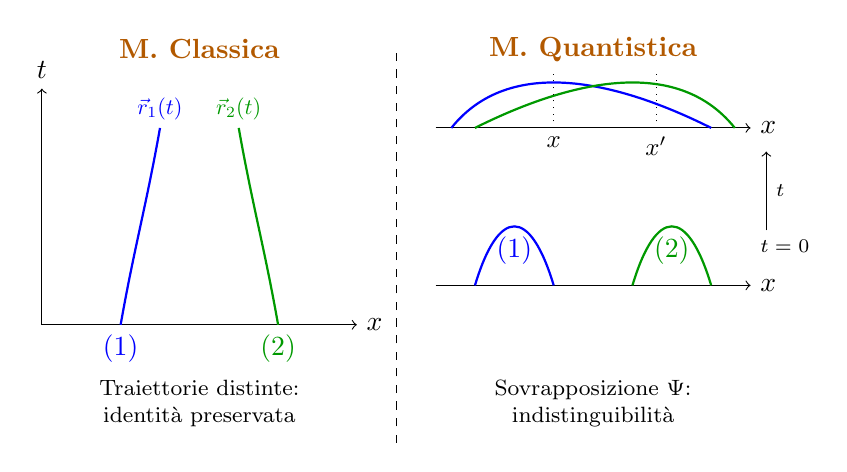
\begin{tikzpicture}
    % Pannello Sinistro: Meccanica Classica
    \begin{scope}[xshift=-4.5cm]
        \node[font=\bfseries, text=orange!70!black] at (2, 3.5) {M. Classica};
        % Assi
        \draw[->] (0,0) -- (4,0) node[right] {$x$};
        \draw[->] (0,0) -- (0,3) node[above] {$t$};
        
        % Traiettorie
        \draw[blue, thick] (1,0) node[below] {(1)} to[out=80, in=260] (1.5,2.5) node[above, scale=0.8] {$\vec{r}_1(t)$};
        \draw[green!60!black, thick] (3,0) node[below] {(2)} to[out=100, in=280] (2.5,2.5) node[above, scale=0.8] {$\vec{r}_2(t)$};
        
        \node[align=center, font=\footnotesize] at (2, -1) {Traiettorie distinte:\\identità preservata};
    \end{scope}

    % Separatore
    \draw[dashed] (0, -1.5) -- (0, 3.5);

    % Pannello Destro: Meccanica Quantistica
    \begin{scope}[xshift=0.5cm]
        \node[font=\bfseries, text=orange!70!black] at (2, 3.5) {M. Quantistica};
        
        % Asse x per t=0
        \draw[->] (0,0.5) -- (4,0.5) node[right] {$x$};
        \node[right] at (4, 1) {\scriptsize $t=0$};
        
        % Pacchetti t=0
        \draw[blue, thick] (0.5,0.5) .. controls (0.8,1.5) and (1.2,1.5) .. (1.5,0.5) node[midway, below] {(1)};
        \draw[green!60!black, thick] (2.5,0.5) .. controls (2.8,1.5) and (3.2,1.5) .. (3.5,0.5) node[midway, below] {(2)};
        
        % Asse x per t > 0
        \draw[->] (0,2.5) -- (4,2.5) node[right] {$x$};
        \draw[->] (4.2, 1.2) -- (4.2, 2.2) node[midway, right] {\scriptsize $t$};
        
        % Pacchetti sovrapposti t > 0
        \draw[blue, thick] (0.2,2.5) .. controls (1,3.5) and (2.5,3) .. (3.5,2.5);
        \draw[green!60!black, thick] (0.5,2.5) .. controls (1.5,3) and (3,3.5) .. (3.8,2.5);
        
        % Punti x e x'
        \draw[dotted] (1.5, 2.5) -- (1.5, 3.2);
        \node[below, scale=0.9] at (1.5, 2.5) {$x$};
        \draw[dotted] (2.8, 2.5) -- (2.8, 3.2);
        \node[below, scale=0.9] at (2.8, 2.5) {$x'$};
        
        \node[align=center, font=\footnotesize] at (2, -1) {Sovrapposizione $\Psi$:\\indistinguibilità};
    \end{scope}
\end{tikzpicture}
\end{center}

% 23 Lezione del 19/11/2025

\lezione{23}{19/11/2025}

Consideriamo ora una particella su uno spazio di Hilbert \(\mathcal{H}\), due insiemi di osservabili I.C.O.C. \(\mathcal{A}\) e \(\mathcal{B}\) e la base di autovettori non degeneri di \(A\) \(\left\{ \ket{a_n} \right\}\).
Se ho due particelle identiche, lo spazio di Hilbert è \(\mathcal{H}\otimes\mathcal{H}= \mathcal{H}^{\otimes2}\) con base ON \(\left\{ \ket{a_{n1}}\otimes \ket{a_{n2}} \right\}\).

Misuriamo \(\mathcal{A}\) su entrambe le particelle, ottenendo due risultati diversi \(a_n\) e \(a_m\). Non sappiamo però su quale particella abbiamo misurato l'uno o l'altro, lo stato dopo la misura sarà dunque:
\[
    \alpha\ket{a_n}\otimes\ket{a_m} + \beta \ket{a_m}\otimes\ket{a_n}
\]
Lo spazio dei vettori compatibile con questa misura ha \(\dim =2\), abbiamo ottenuto della \textit{degenerazione di scambio}.



Consideriamo il caso in cui, dopo aver misurato l'osservabile \( A \), si misuri \( B \). Ci chiediamo quale sia la probabilità che la misura di \( B \) dia due valori diversi per le due particelle \( b_i \neq b_j \).\\
Non sapendo quale sia lo stato del sistema scegliamo arbitrariamente tra \(\ket{a_n}\otimes\ket{a_m} \) e \( \ket{a_m}\otimes\ket{a_n}\).
La probabilità di transizione partendo da uno stato fattorizzato \( \ket{a_n}\otimes\ket{a_m} \) è data dal modulo quadro del prodotto scalare:
\[
    \text{Prob}_{\ket{a_n}\otimes\ket{a_m}}(b_i, b_j) = \abs{(\bra{b_i}\otimes\bra{b_j})(\ket{a_n}\otimes\ket{a_m})}^2
    = \abs{\braket{b_i}{a_n}}^2 \abs{\braket{b_j}{a_m}}^2
\]

Se avessi scelto l'ordine opposto \( \ket{a_m}\otimes\ket{a_n} \), avrei ottenuto:
\[
    \text{Prob}_{\ket{a_m}\otimes\ket{a_n}}(b_i, b_j) = \abs{\braket{b_i}{a_m}}^2 \abs{\braket{b_j}{a_n}}^2
\]

Notiamo che otteniamo probabilità diverse! Quindi le probabilità dipendono dal vettore iniziale scelto. Tuttavia:
\begin{itemize}
    \item Solo una scelta è quella giusta, le altre portano a probabilità sbagliate che non osservo in laboratorio e quindi a risultati teorici errati.
    \item Le particelle sono indistinguibili: le etichette \( (1) \) o \( (2) \) non sono osservabili.
\end{itemize}
Come scegliere, dunque,il vettore iniziale giusto?
Per una particella singola la base è \( \{ \ket{e_n} \} \). Per due particelle lo spazio di Hilbert è il prodotto tensore \( \mathcal{H} \otimes \mathcal{H} = \mathcal{H}^{\otimes 2} \) 
con base \( \{ \ket{e_n}\otimes\ket{e_m} \} \), le nostre teorie devono essere invarianti per lo scambio delle etichette 1 e 2.\\
Formalizziamo meglio questo concetto.

\subsection{Simmetria di Scambio}
Definiamo un operatore unitario su \(\mathcal{H}\) detto \textit{operatore di scambio}:
\begin{equation}
    \hat{P}_{1,2} ( \ket{u}\otimes\ket{v} ) = \ket{v}\otimes\ket{u}
\end{equation}

\textbf{Proprietà:}
\begin{itemize}
    \item Il dominio è \( D(\hat{P}_{12}) = \mathcal{H} \otimes \mathcal{H} \) e l'immagine è \( \hat{P}_{12}(\mathcal{H} \otimes \mathcal{H}) = \mathcal{H} \otimes \mathcal{H} \).
    \item Conserva la norma: \( \norm{\hat{P}_{12}\ket{\Psi}}^2 = \norm{\ket{\Psi}}^2 \).
    \item 
    \(
    \hat{P}_{12}^2 = I \implies \hat{P}_{12} = \hat{P}_{12}^{-1} = \hat{P}_{12}^\dagger \implies \hat{P}_{12} \text{ è a.a.}
    \)
    \item Lo spettro è discreto: \( \sigma(\hat{P}_{12}) = \{ \pm 1 \} \).
\end{itemize}

Possiamo dunque decomporre lo spazio prodotto tensore come somma diretta dei sottospazi relativi agli autovalori:
\[
\mathcal{H}^{\otimes 2} = \mathcal{H}_S \oplus \mathcal{H}_A
\]
dove:
\begin{itemize}
    \item \( \mathcal{H}_S \) (autovalore \( +1 \)): sottospazio simmetrico, \( \hat{P}_{12} \) lascia invariati i vettori qui dentro.
    \item \( \mathcal{H}_A \) (autovalore \( -1 \)): sottospazio antisimmetrico, \( \hat{P}_{12} \) cambia segno ai vettori.
\end{itemize}

\begin{postulato9}
    Dato uno stato fisico rappresentato dal raggio vettore \(\left[ \Psi \right]\), lo scambio di etichette deve lasciare lo stato invariato:
    \begin{equation}
        \left[ \Psi \right]= \left[ \hat{P}_{12} \ket{\Psi}\right]
    \end{equation}
    Dunque: \[
        \hat{P}_{12} \Psi= c_\Psi\ket{\Psi}\,, \ c_\Psi \in \left\{ \pm 1  \right\} \implies \ket{\Psi} \in \mathcal{H}_S \ \text{ o } \ \ket{\Psi} \in \mathcal{H}_A
    \]
\end{postulato9}

\begin{definition}
    Per \(\ket{\Psi} \in \mathcal{H}^{\otimes 2}\) stato fisico di 2 particelle identiche:
    \begin{itemize}
        \item Se \(\ket{\Psi}\in \mathcal{H}_S\), la particella si dice \textit{bosone}.
        \item Se \(\ket{\Psi}\in \mathcal{H}_A\), la particella si dice \textit{fermione}.
    \end{itemize}
\end{definition}

\begin{theorem}
    { \normalfont \textbf{Spin-statistica}}\\
    Una particella di spin \(s \) è un bosone se e solo se \(s \in \mathbb{N}\) o un fermione se e solo se \(s \in \frac{1}{2} + \mathbb{N}\) .
\end{theorem}


Non tutti gli operatori a.a. su \(\mathcal{H}^{\otimes 2}\) corrispondono a un osservabile, un generico operatore \(A = \sum_i B_i\otimes C_i\) definisce un osservabile fisico solo se è invariante per scambio etichette:
\[
    \forall \ket{\Psi} \in \mathcal{H}_S \implies A\ket{\Psi} \in \mathcal{H}_S \qquad 
    \forall \ket{\Psi} \in \mathcal{H}_A \implies A\ket{\Psi} \in \mathcal{H}_A 
\]
\[
    \iff \hat{P}_{12} A \hat{P}^\dagger_{12} = A \iff \left[ A, \hat{P}_{12} \right]=0
\]

\begin{remark}
    Nota che l'azione dell'operatore di scambio sugli operatori tensoriali è data da:
    \[
    \hat{P}_{12} \left( \sum_{i} B_i \otimes C_i \right) \hat{P}_{12}^\dagger = \sum_{i} C_i \otimes B_i
    \]
\end{remark}
\begin{example}
    Se \( B \neq C \), allora:
    \begin{itemize}
        \item \( B \otimes C - C \otimes B \) e \( B \otimes C \) non sono osservabili (perché non simmetrici rispetto allo scambio).
        \item \( B \otimes B \), \( C \otimes C \) e \( B \otimes C + C \otimes B \) sono osservabili.
    \end{itemize}
\end{example}

\begin{remark}
    E' essenziale che anche $H$ sia invariante \quad $\hat{P}_{12} H \hat{P}_{12} = H$\\
    Questa condizione implica che la simmetria (o antisimmetria) dello stato venga preservata durante l'evoluzione temporale:
    \[
    \implies \text{se } \ket{\psi} \in 
    \begin{matrix}
        \mathcal{H}_S \\ \mathcal{H}_A
    \end{matrix} 
    \quad \implies \quad 
    U(t, t_0)\ket{\psi} \in 
    \begin{matrix}
        \mathcal{H}_S \\ \mathcal{H}_A
    \end{matrix}
    \]
\end{remark}

\begin{example}
    Un esempio tipico di Hamiltoniana per due particelle identiche è:
    \[
    H = \frac{\vec{P}_1^2}{2m} + \frac{\vec{P}_2^2}{2m} + V(\vec{X}_1, \vec{X}_2)
    \]
    dove il potenziale di interazione deve essere simmetrico rispetto allo scambio delle coordinate delle particelle:
    \[
    V(\vec{X}_1, \vec{X}_2) = V(\vec{X}_2, \vec{X}_1)
    \]
\end{example}

Grazie al postulato posso risolvere il problema della degenerazione di scambio: se misuro \(A\) su entrambe le particelle e ottengo due risultati \(a_n \neq a_m\), 
l'unica combinazione lineare ammissibile per i bosoni è quella simmetrica:
\begin{equation}
    \frac{1}{\sqrt{2}}\left( \ket{a_n}\otimes\ket{a_m} + \ket{a_n}+ \ket{a_m} \right)  \in \mathcal{H}_S
\end{equation}
Mentre per i fermioni è quella antisimmetrica:
\begin{equation}
    \frac{1}{\sqrt{2}}\left( \ket{a_n}\otimes\ket{a_m} - \ket{a_n}+ \ket{a_m} \right)  \in \mathcal{H}_A
\end{equation}

\begin{attention}
    Cosa succede se le due particelle dovessero trovarsi nello stesso stato \(\Psi \in \mathcal{H}\)? Per i bosoni non è un problema \(\ket{\Psi}\otimes\ket{\Psi} \in \mathcal{H}_S\),
    per i fermioni non esiste una combinazione lineare antisimmetrica!
\end{attention}

\begin{pauli}
    \label{theo: Pauli}
    Se ho due fermioni identici non possono essere nello stesso stato di particella singola.
\end{pauli}


\subsection{Caso N particelle identiche}
Consideriamo uno spazio di Hilbert \(\mathcal{H}^{\otimes N}= \mathcal{H}\otimes...\otimes \mathcal{H}\) con base \(\left\{ \ket{e_{n_1}}\ket{e_{n_2}}...\ket{e_{n_N}} \right\}\) (dove abbiamo omesso il simbolo \(\otimes\) per convenienza), i vettori sono descritti da:
\begin{equation}
    \ket{\Psi} = \sum_{n_1,n_2,...,n_N}c_{n_1,n_2,..., n_N}\ket{e_{n_1}}\ket{e_{n_2}}...\ket{e_{n_N}}
\end{equation}
Vogliamo che la fisica sia invariante per qualsiasi scambio di etichette, cioè permutazioni del tipo:
\begin{equation}
    \pi : \left\{ 1,2,...,N \right\}\to \left\{ 1,2,..., N \right\}
\end{equation}
Consideriamo dunque il gruppo delle permutazioni invertbili \(S_N\) .
\begin{remark}
    Il gruppo \(S_N\) ha \(N!\) elementi ed è non-abeliano se \(N\geq 3\) .
\end{remark}

Per ogni scambio ho un operatore unitario che agisce nel seguente modo:
\begin{align*}
    S_N \ni \pi \rightsquigarrow \hat{P}_{\pi}\ket{\Psi} &=\hat{P}_{\pi} \left( \sum_{n_1, \dots, n_N} c_{n_1, \dots, n_N} \ket{e_{n_1}} \ket{e_{n_2}} \dots \ket{e_{n_N}} \right) \\
    &=\sum_{n_1, \dots, n_N} c_{n_1, \dots, n_N} \ket{e_{n_{\pi^{-1}(1)}}} \ket{e_{n_{\pi^{-1}(2)}}} \dots \ket{e_{n_{\pi^{-1}(N)}}}
\end{align*}

L'azione sui singoli vettori prodotto è quindi:
\[
\hat{P}_{\pi} \ket{u_1} \dots \ket{u_N} = \ket{u_{\pi^{-1}(1)}} \ket{u_{\pi^{-1}(2)}} \dots \ket{u_{\pi^{-1}(N)}}
\]

Ottengo così gli operatori \(\hat{P}_{\pi} \) per cui vale \(\hat{P}_{\pi} \hat{P}_{\pi'}= \hat{P}_{\pi\circ \pi'}\) e \(\hat{P}_{\pi}^\dagger = \hat{P}_{\pi}^{-1}= \hat{P}_{\pi^{-1}} \),
i \(\hat{P}_{\pi} \) sono dunque rapresentazione unitaria non proiettiva di \(S_N\).
\begin{remark}
    Si è definita l'azione di \(\hat{P}_{\pi} \) usando la permutazione inversa \(\pi^{-1}\) perché altrimenti \(\hat{P}_{\pi} \hat{P}_{\pi'}= \hat{P}_{\pi\circ \pi'}\) avrebbe le composizione al contrario e non sarebbe lo stesso gruppo. 
\end{remark}


\begin{postulato9}
    {\normalfont (Caso generale)}\\
    Consideriamo \( N \) particelle identiche, \( \ket{\Psi} \in \mathcal{H}^{\otimes N} \) rappresenta uno stato fisico se e solo se:
    \begin{equation}
        \forall \pi \in S_N \quad \hat{P}_{\pi} \ket{\Psi} = c_{\pi}(\Psi) \ket{\Psi}
    \end{equation}
\end{postulato9}
Si nota che:
\begin{itemize}
        \item Deve valere \( |c_{\pi}(\Psi)| = 1 \).
        \item Se voglio che \( \forall \Psi, \Psi' \) fisici, anche la sovrapposizione \( \Psi + \Psi' \) sia uno stato fisico \( \implies c_{\pi}(\Psi) = c_{\pi}(\Psi') \) (cioè la costante \( c \) non dipende dallo specifico stato \( \Psi \)).
\end{itemize}




Consideriamo un particolare caso di permutazioni, le trasposizioni \(\pi_{ij}\) cambiano solo 2 elementi dell'insieme lasciando invariati gli altri:
\[
\begin{matrix}
1 & \longrightarrow & 1 \\
\vdots & & \vdots \\
i & \longrightarrow & j \\
\vdots & & \vdots \\
j & \longrightarrow & i \\
\vdots & & \vdots \\
N & \longrightarrow & N
\end{matrix}
\]

Qualunque permutazione la ottengo componendo trasposizioni:
\[
\forall \pi \in S_N, \quad \pi = \pi_{i_1 j_1} \circ \pi_{i_2 j_2} \circ \dots \circ \pi_{i_\ell j_\ell}
\]
Da cui segue la scomposizione per gli operatori:
\[
\hat{P}_{\pi} = \hat{P}_{i_1 j_1} \dots \hat{P}_{i_\ell j_\ell}
\]

\begin{remark}
    La decomposizione di una permutazione \( \pi \) in trasposizioni non è unica.
    Ciò implica che il numero di trasposizioni \( \ell \) può essere diverso, ma tutte le decomposizioni avranno la stessa parità.
\end{remark}

\begin{definition}
    Una permutazione \( \pi \) è detta \textit{pari/dispari} se e solo se il numero di trasposizioni \( \ell \) nella sua decomposizione è pari/dispari.
\end{definition}

Essendo gli autovalori di una singola trasposizione \(\left\{ \pm 1 \right\}\) gli unici autovalori possibili per una permutazione sono:

\begin{enumerate}
    \item \( c_{\pi} = +1 \quad \forall \pi \in S_N \)
    \item \( c_{\pi} = \mathrm{Sgn}(\pi) = 
    \begin{cases}
        +1 & \text{se } \pi \text{ è pari} \\
        -1 & \text{se } \pi \text{ è dispari}
    \end{cases}
    \)
\end{enumerate}


\begin{theorem}
    { \normalfont \textbf{Spin-statistica}}\\
    \(N\) particelle identiche sono bosoni \(s \in \mathbb{N}\) se e solo se:
    \begin{equation}
        \hat{P}_{\pi}\ket{\Psi}= +\ket{\Psi} \quad  \forall\,\pi \in S_N \iff \ket{\Psi}\in \mathcal{H}_S \subseteq \mathcal{H}^{\otimes N}
    \end{equation}
    \(N\) particelle identiche sono fermioni \(s \in \frac12 + \mathbb{N}\) se e solo se:
    \begin{equation}
        \hat{P}_{\pi}\ket{\Psi}= \mathrm{Sgn}(\pi)\ket{\Psi} \quad  \forall\,\pi \in S_N \iff \ket{\Psi}\in \mathcal{H}_A \subseteq \mathcal{H}^{\otimes N}
    \end{equation}
\end{theorem}

\begin{remark}
    \(\mathcal{H}^{\otimes N}= \mathcal{H}_S \oplus \mathcal{H}_A \oplus \dots\) le altre componenenti sono spazi di Hilbert di stati non fisici.
\end{remark}

% 24 Lezione del 21/11/2025

\begin{example}
    \textbf{\(N=3\)}\\
    \lezione{24}{21/11/2025}
    Analizziamo la costruzione degli stati fisici per un sistema di 3 particelle identiche a partire dagli stati di singola particella.
    Per particelle bosoniche gli stati devono essere completamente simmetrici sotto scambio di particelle, ovvero invarianti per ogni permutazione \(\pi\).
    \begin{itemize}
        \item \textbf{3 particelle nello stesso stato \(\ket{u}\):}
        \[
            \ket{u}\otimes\ket{u}\otimes\ket{u} = \ket{u}\ket{u}\ket{u}
        \]
        Questo stato è già invariante per qualsiasi permutazione, quindi appartiene a \(\mathcal{H}_S\).

        \item \textbf{2 particelle in \(\ket{u}\) e 1 in \(\ket{v}\):}
        Preso singolarmente, \(\ket{u}\ket{u}\ket{v}\) non è uno stato fisico per particelle indistinguibili. Dobbiamo costruire una combinazione lineare simmetrica sommando le permutazioni distinte:
        \[
            \frac{1}{\sqrt{3}}\left( \ket{u}\ket{u}\ket{v} + \ket{u}\ket{v}\ket{u} + \ket{v}\ket{u}\ket{u} \right) \in \mathcal{H}_S
        \]
        dove \(\frac{1}{\sqrt{3}}\) è il fattore di normalizzazione.

        \item \textbf{3 particelle in stati tutti diversi \(\ket{a}, \ket{b}, \ket{c}\):}
        Per ottenere una combinazione simmetrica appartenente a \(\mathcal{H}_S\), dobbiamo sommare su tutte le permutazioni possibili (\(3! = 6\)):
        \[
            \frac{1}{\sqrt{6}}\Big( \ket{a}\ket{b}\ket{c} + \ket{b}\ket{c}\ket{a} + \ket{c}\ket{a}\ket{b} + \ket{b}\ket{a}\ket{c} + \ket{a}\ket{c}\ket{b} + \ket{c}\ket{b}\ket{a} \Big) \in \mathcal{H}_S
        \]
        In generale, otteniamo lo stato fisico sommando sulle permutazioni \(\pi \in S_N\) tramite l'operatore di permutazione \(\hat{P}_\pi\):
        \[
            \mathcal{N} \sum_{\pi \in S_N} \hat{P}_\pi \ket{a}\ket{b}\ket{c} \in \mathcal{H}_S
        \]
    \end{itemize}

    Se vogliamo rappresentare dei fermioni, lo stato deve essere totalmente antisimmetrico e appartenere a \(\mathcal{H}_A\). La somma diventa una somma alternante, con segno positivo per le permutazioni pari e negativo per quelle dispari:
    \[
        \frac{1}{\sqrt{6}}\Big( \ket{a}\ket{b}\ket{c} + \ket{b}\ket{c}\ket{a} + \ket{c}\ket{a}\ket{b} - \ket{b}\ket{a}\ket{c} - \ket{a}\ket{c}\ket{b} - \ket{c}\ket{b}\ket{a} \Big) \in \mathcal{H}_A
    \]
    La formula generale coinvolge la segnatura della permutazione \(\operatorname{sgn}(\pi)\):
    \[
        \mathcal{N} \sum_{\pi \in S_N} \operatorname{sgn}(\pi) \hat{P}_\pi \ket{a}\ket{b}\ket{c} \in \mathcal{H}_A
    \]
    \begin{attention}
        Se avessimo due stati uguali (ad esempio \(\ket{a} = \ket{b}\)), i termini con segno opposto si cancellerebbero a vicenda annullando l'intera somma.
        Questo risultato costituisce l'estensione del \textit{Principio di esclusione di Pauli} ( \ref{theo: Pauli}): non possono esserci due fermioni nello stesso stato quantico.
    \end{attention}
\end{example}

\subsubsection{Osservabili fisici}
Le osservabili fisiche sono rappresentate da operatori autoaggiunti \(A: \mathcal{H}^{\otimes N} \to \mathcal{H}^{\otimes N}\) che commutano con ogni operatore di permutazione:
    \begin{equation}
        [A, \hat{P}_\pi] = 0 \quad \forall \pi \in S_N
    \end{equation}
    Questa condizione è equivalente a richiedere che l'operatore sia invariante sotto coniugazione per una qualsiasi permutazione:
    \begin{equation}
        \hat{P}_\pi A \hat{P}_\pi^\dagger = A \quad \forall \pi \in S_N
    \end{equation}
In particolare, questa proprietà deve valere per l'operatore Hamiltoniano del sistema:
    \begin{equation}
        \hat{P}_\pi H \hat{P}_\pi^\dagger = H \quad \forall \pi \in S_N
    \end{equation}

\begin{attention}
    Le osservabili devono essere sempre \textbf{simmetriche} rispetto allo scambio di particelle, a differenza degli stati (che possono essere antisimmetrici nel caso dei fermioni).
\end{attention}

\begin{example}
    Consideriamo un esempio con 3 particelle e due operatori di singola particella \(A\) e \(B\). Vogliamo costruire un operatore globale simmetrico.
    La combinazione:
    \[
        \mathcal{O} = A\otimes A \otimes B + A\otimes B \otimes A + B\otimes A \otimes A
    \]
    è corretta. Se, per esempio, agisco con l'operatore di permutazione \(\hat{P}_{23}\) (scambio tra la particella 2 e 3):
    \begin{itemize}
        \item \(A\otimes \mathbf{A} \otimes \mathbf{B} \xrightarrow{\hat{P}_{23}} A\otimes \mathbf{B} \otimes \mathbf{A}\)
        \item \(A\otimes \mathbf{B} \otimes \mathbf{A} \xrightarrow{\hat{P}_{23}} A\otimes \mathbf{A} \otimes \mathbf{B}\)
        \item \(B\otimes \mathbf{A} \otimes \mathbf{A} \xrightarrow{\hat{P}_{23}} B\otimes \mathbf{A} \otimes \mathbf{A}\)
    \end{itemize}
    Se permuto gli elementi, la somma totale rimane uguale, quindi l'operatore è simmetrico.
\end{example}

\subsection{Sistema a due elettroni e composizione degli spin}

Consideriamo un sistema composto da 2 elettroni ($2\,e^-$). Lo spazio di Hilbert totale è il prodotto tensore degli spazi delle singole particelle:
\begin{itemize}
    \item Spazio di Hilbert della 1° particella: \(\mathcal{H}_1 = \mathcal{H}_{\vec{x}_1} \otimes \mathcal{H}_{s_1}\)
    \item Spazio di Hilbert della 2° particella: \(\mathcal{H}_2 = \mathcal{H}_{\vec{x}_2} \otimes \mathcal{H}_{s_2}\)
\end{itemize}
Per comodità, possiamo raggruppare la parte spaziale e la parte di spin:
\[
    \mathcal{H}^{tot} = (\mathcal{H}_{\vec{x}_1} \otimes \mathcal{H}_{s_1}) \otimes (\mathcal{H}_{\vec{x}_2} \otimes \mathcal{H}_{s_2}) 
    \cong \underbrace{(\mathcal{H}_{\vec{x}_1} \otimes \mathcal{H}_{\vec{x}_2})}_{\mathcal{H}^{pos}} \otimes \underbrace{(\mathcal{H}_{s_1} \otimes \mathcal{H}_{s_2})}_{\mathcal{H}^{spin}}
\]
Dove:
\begin{itemize}
    \item \(\mathcal{H}^{pos} \cong L_2(\mathbb{R}^3 \times \mathbb{R}^3, d^3x_1 d^3x_2)\)
    \item \(\mathcal{H}^{spin} \cong \mathbb{C}^2 \otimes \mathbb{C}^2\) (dimensione totale \(2\times2=4\))
\end{itemize}

Come già visto abbiamo due possibili scelte per l'insieme completo di osservabili che commutano (I.C.O.C.):
\begin{itemize}
    \item Utilizzando gli spin individuali.
    \[
        \{\vec{X}_1, \vec{X}_2, S_{1z}, S_{2z}\} \quad \longrightarrow \quad \ket{\vec{x}_1, \vec{x}_2, m_1, m_2}
    \]
    
    \item Utilizzando lo spin totale del sistema \(\vec{S} = \vec{S}_1 + \vec{S}_2\).
    \[
        \{\vec{X}_1, \vec{X}_2, \vec{S}^2, S_z\} \quad \longrightarrow \quad \ket{\vec{x}_1, \vec{x}_2, S, m}
    \]
\end{itemize}

\subsubsection{Stati di Singoletto e Tripletto}
Effettuiamo il cambio di base per la parte di spin. Avendo \(s_1 = 1/2\) e \(s_2 = 1/2\), lo spin totale \(S\) può assumere valori nell'intervallo \(|s_1 - s_2| \le S \le s_1 + s_2\), ovvero \(S \in \{1, 0\}\).
I 4 stati possibili si raggruppano in:

\paragraph{Tripletto (\(S=1\))}
Spin totale del sistema \(1\), simmetrico per scambio. Ci sono 3 stati (\(m=1, 0, -1\)):
\begin{equation}
    \begin{cases}
        \ket{1, 1} = \ket{+ +} \\
        \ket{1, 0} = \frac{1}{\sqrt{2}} \left( \ket{+ -} + \ket{- +} \right) \\
        \ket{1, -1} = \ket{- -}
    \end{cases}
\end{equation}
Lo stato \(\ket{1,0}\) si ottiene applicando l'operatore di abbassamento \(S_-\) allo stato \(\ket{1,1}\).

\paragraph{Singoletto (\(S=0\))}
Spin totale nullo, antisimmetrico per scambio. C'è un solo stato (\(m=0\)), che deve essere ortogonale a \(\ket{1,0}\):
\begin{equation}
    \ket{0, 0} = \frac{1}{\sqrt{2}} \left( \ket{+ -} - \ket{- +} \right)
\end{equation}
Questo stato appare solo una volta poiché \(S\) ha un solo valore disponibile (\(s_1 - s_2 = 0\)).

Uno stato generico \(\ket{\Psi}\) in \(\mathcal{H}^{\otimes 2}\) può essere scritto espandendo sulla base accoppiata:
\begin{equation}
    \ket{\Psi} = \sum_{S=0}^{1} \sum_{m=-S}^{S} \Psi_{S,m}(\vec{x}_1, \vec{x}_2) \ket{S, m}
        \equiv \sum_{S,m} \Psi_{S,m}(\vec{x}_1, \vec{x}_2) \otimes \ket{S, m}
\end{equation}
dove le \(\Psi_{S,m}(\vec{x}_1, \vec{x}_2) = \braket{\vec{x}_1, \vec{x}_2, S, m}{\Psi}\) sono 4 funzioni d'onda spaziali che specificano lo stato.

Poiché sono fermioni, la funzione d'onda totale $\ket{\Psi}$ deve essere antisimmetrica rispetto allo scambio delle particelle. Definito l'operatore di scambio $\hat{P}_{12}$, deve valere:
\[
    \hat{P}_{12} \ket{\Psi} = - \ket{\Psi}
\]

L'operatore di scambio agisce sia sui gradi di libertà spaziali che su quelli di spin. Possiamo scriverlo come prodotto tensore:
\[
    \hat{P}_{12} = \hat{P}_{12}^{pos} \otimes \hat{P}_{12}^{spin}
\]

Analizziamo l'azione separata delle due componenti:
\begin{itemize}
    \item \textbf{Parte spaziale:} scambia le coordinate delle due particelle:
    \[
    \hat{P}_{12}^{pos} \Psi(\vec{x}_1, \vec{x}_2) = \Psi(\vec{x}_2, \vec{x}_1)
    \]
    \item \textbf{Parte di spin:} scambia i numeri quantici di spin $m_1$ e $m_2$:
    \[
    \hat{P}_{12}^{spin} \ket{m_1, m_2} = \ket{m_2, m_1}
    \]
\end{itemize}


L'azione di $\hat{P}_{12}^{spin}$ dipende dallo stato di spin totale $S$ del sistema:
\begin{itemize}
    \item Per lo stato di \textbf{Tripletto} ($S=1$), lo stato è simmetrico per scambio:
    \[
    \hat{P}_{12}^{spin} \ket{1, m} = + \ket{1, m}
    \]
    \item Per lo stato di \textbf{Singoletto} ($S=0$), lo stato è antisimmetrico per scambio:
    \[
    \hat{P}_{12}^{spin} \ket{0, 0} = - \ket{0, 0}
    \]
\end{itemize}

Imponiamo ora la condizione che lo stato fisico complessivo sia antisimmetrico:
\[
    \hat{P}_{12} \ket{\Psi_{S,m}} = \left( \hat{P}_{12}^{pos} \otimes \hat{P}_{12}^{spin} \right) \left( \Psi_{space} \otimes \ket{S,m} \right) = - \ket{\Psi_{S,m}}
\]
Affinché il totale sia negativo, le simmetrie spaziali e di spin devono essere opposte.


Per lo stato di tripleto (\(s=1\)), la parte di spin è simmetrica ($+$). Di conseguenza, la parte spaziale deve essere \textbf{antisimmetrica} ($-$) per ottenere un segno totale negativo:
\[
    \implies \Psi_{S=1, m}(\vec{x}_2, \vec{x}_1) = - \Psi_{S=1, m}(\vec{x}_1, \vec{x}_2)
\]

Invece per lo stato di singoletto (\(s=0\)), la parte di spin è antisimmetrica ($-$). Di conseguenza, la parte spaziale deve essere \textbf{simmetrica} ($+$):
\[
    \implies \Psi_{S=0, 0}(\vec{x}_2, \vec{x}_1) = + \Psi_{S=0, 0}(\vec{x}_1, \vec{x}_2)
\]

\subsubsection{Effetto fisico di funzioni d'onda simmetirce e antisimmetriche}

Consideriamo due funzioni d'onda di particella singola \(\psi_A(\vec{x}), \psi_B(\vec{x}) \in L_2(\mathbb{R}^3)\), con \(\psi_A \neq \psi_B\):
\begin{equation}
    \int \abs{\psi_{A,B}(\vec{x})}^2 \dd[3]{x} = 1 \qquad \braket{\psi_A}{\psi_B} = 0
\end{equation}

Supponiamo di avere due \(e^-\), uno con funzione d'onda \(\psi_A\) e uno con funzione d'onda \(\psi_B\) (e qualche stato di spin). 
La funzione d'onda spaziale totale sarà:
\begin{equation}
    \Psi_{\substack{S=0 \\ S=1}} (\vec{x}_1, \vec{x}_2) = \frac{1}{\sqrt{2}} \left( \psi_A(\vec{x}_1) \psi_B(\vec{x}_2) \pm \psi_A(\vec{x}_2) \psi_B(\vec{x}_1) \right)
\end{equation}
Il più per le funzioni d'onda simmetriche e il meno per le funzioni d'onda antisimmetriche. Entrambe le funzioni sono normalizzate:
\[
    \int \abs{\Psi(\vec{x}_1, \vec{x}_2)}^2 \dd[3]{x_1} \dd[3]{x_2} = 1
\]

Calcoliamo la probabilità di trovare entrambe le particelle nella stessa posizione \(\vec{x}_1 = \vec{x} = \vec{x}_2\):
\begin{equation}
    \rho(\vec{x}, \vec{x}) = \abs{\Psi(\vec{x}, \vec{x})}^2
\end{equation}

Analizziamo i tre casi possibili:

\begin{enumerate}
    \item \textbf{\(\Psi\) simmetrica}:
    \begin{equation}
        \rho_S(\vec{x}, \vec{x}) = \abs{\frac{1}{\sqrt{2}} \left( 2\psi_A(\vec{x})\psi_B(\vec{x}) \right)}^2 = \frac{1}{2} \cdot 4 \abs{\psi_A(\vec{x})}^2 \abs{\psi_B(\vec{x})}^2 = 2 \abs{\psi_A(\vec{x})}^2 \abs{\psi_B(\vec{x})}^2
    \end{equation}
    La probabilità è doppia rispetto al caso di particelle distinguibili (attrazione efficace).

    \item \textbf{\(\Psi\) antisimmetrica}:
    \begin{equation}
        \rho_A(\vec{x}, \vec{x}) = \abs{\frac{1}{\sqrt{2}} \left( \psi_A(\vec{x})\psi_B(\vec{x}) - \psi_A(\vec{x})\psi_B(\vec{x}) \right)}^2 = 0
    \end{equation}
    La probabilità è nulla: principio di esclusione di Pauli (repulsione efficace).

    \item \textbf{Particelle distinguibili}:
    \begin{equation}
        \Psi_D(\vec{x}_1, \vec{x}_2) = \psi_A(\vec{x}_1)\psi_B(\vec{x}_2)\implies 
            \rho_D(\vec{x}, \vec{x}) = \abs{\psi_A(\vec{x})}^2 \abs{\psi_B(\vec{x})}^2
    \end{equation}
\end{enumerate}

Calcoliamo ora invece la probabilità che le particelle si trovino in posizioni differenti \(\vec{x}\neq \vec{x}'\):

\begin{enumerate}
    \item \textbf{\(\Psi\) Simmetrica o Antisimmetrica (Indistinguibili)}:
    Poiché \(\Psi\) è (anti)simmetrica, il modulo quadro è invariante per lo scambio delle coordinate:
    \begin{equation}
        \abs{\Psi(\vec{x}, \vec{x}')}^2 = \abs{\Psi(\vec{x}', \vec{x})}^2
    \end{equation}
    Quindi la densità totale diventa:
    \[
        \rho_{S,A}^{tot}(\vec{x}, \vec{x}') = 2 \cdot \abs{\Psi(\vec{x}, \vec{x}')}^2 = 2 \cdot \frac{1}{2} \abs{\psi_A(\vec{x})\psi_B(\vec{x}') \pm \psi_A(\vec{x}')\psi_B(\vec{x})}^2
    \]
    Espandendo il modulo quadro:
    \[
        = \abs{\psi_A(\vec{x})}^2 \abs{\psi_B(\vec{x}')}^2 + \abs{\psi_A(\vec{x}')}^2 \abs{\psi_B(\vec{x})}^2 \pm 2 \Re\left( \psi_A^*(\vec{x})\psi_B^*(\vec{x}')\psi_A(\vec{x}')\psi_B(\vec{x}) \right)
    \]
    Il termine aggiuntivo:
    \begin{equation}
        \pm 2 \Re\left( \psi_A^*(\vec{x})\psi_B^*(\vec{x}')\psi_A(\vec{x}')\psi_B(\vec{x}) \right)
    \end{equation}
    rappresenta l'\textbf{interazione di scambio}.

    \item \textbf{Particelle Distinguibili}:
    Per particelle classiche o distinguibili, non c'è simmetrizzazione:
    \begin{equation}
        \rho_D^{tot}(\vec{x}, \vec{x}') = \abs{\psi_A(\vec{x})}^2 \abs{\psi_B(\vec{x}')}^2 + \abs{\psi_A(\vec{x}')}^2 \abs{\psi_B(\vec{x})}^2
    \end{equation}
\end{enumerate}

\begin{example}
    Se abbiamo un \(e^-\) sulla Terra e un altro sulla Luna, devo anti-simmetrizzare il loro stato?

Siano \(\psi_A(\vec{x})\) a supporto in \(R_A\) (Terra) e \(\psi_B(\vec{x})\) a supporto in \(R_B\) (Luna), tali che \(R_A \cap R_B = \emptyset\).
\[
    \psi_{A,B}(\vec{x}) = 0 \quad \forall \vec{x} \notin R_{A,B}
\]

Verifichiamo la probabilità che si trovino nello stesso punto:
\[
    \rho(\vec{x}, \vec{x}) \propto \abs{\psi_A(\vec{x})}^2 \abs{\psi_B(\vec{x})}^2 = 0 \quad \forall \vec{x}
\]
Infatti:
\begin{itemize}
    \item Se \(\vec{x} \in R_A \implies \psi_B(\vec{x}) = 0\)
    \item Se \(\vec{x} \in R_B \implies \psi_A(\vec{x}) = 0\)
    \item Se \(\vec{x} \notin R_A \cup R_B \implies \psi_{A,B}(\vec{x}) = 0\)
\end{itemize}

Il termine di interferenza (scambio) si annulla identicamente:
\[
    2\Re \left( \psi_A^*(\vec{x})\psi_B^*(\vec{x}') \psi_A(\vec{x}')\psi_B(\vec{x}) \right) = 0 \quad \forall \vec{x}, \vec{x}'
\]
Questo perché per ogni coppia \((\vec{x}, \vec{x}')\), almeno uno dei fattori nel prodotto incrociato è nullo (non c'è sovrapposizione delle funzioni d'onda).

\[
    \rho_S^{tot}(\vec{x}, \vec{x}') = \rho_A^{tot}(\vec{x}, \vec{x}') = \rho_D^{tot}(\vec{x}, \vec{x}')
\]
Non commetto alcun errore se le tratto come particelle \textbf{distinguibili}.
\end{example}


\chapter{Atomo di idrogeno}


\section{Potenziali Centrali}

Ignoriamo lo spin (\( \vec{S}=0 \implies \vec{J}=\vec{L} \)), tutte le osservabili sono funzioni di posizione e momento. Consideriamo un potenziale dipendente solo dalla distanza centro-punto (raggio):
\[
H = \frac{\vec{P}^2}{2m} + V(R) \qquad R = \sqrt{\vec{X}^2}
\]
L'operatore \( R \) agisce come moltiplicazione per la distanza:
\[
R\ket{\vec{x}} = \abs{\vec{x}}\ket{\vec{x}}
\]
Calcoliamo i commutatori con il momento angolare \( \vec{L} \):
\[
[\vec{L}, \vec{P}^2] = 0 = [\vec{L}, \vec{X}^2] = [\vec{L}, V(R)]
\]
Questo implica che l'hamiltoniana è invariante per rotazioni (\( SO(3) \to \) simmetria dinamica) e commuta con tutte e tre le componenti di \( \vec{L} \):
\[
[\vec{L}, H] = 0
\]

\begin{remark}
    Se \([P_i, V(\vec{x})] = 0 \implies V(\vec{x})\) non dipende da \( X_i \implies \) si riduce ad un problema in \(\dim < 3\).
\end{remark}

Poiché \( H \) commuta con \( \vec{L} \), possiamo diagonalizzare simultaneamente \( \{H, \vec{L}^2, L_z\} \). Questi formano un insieme di osservabili compatibili.
Possiamo dunque risolvere l'equazione agli autovalori simultaneamente per \( H \) , \( \vec{L}^2 \) e \(L_z\). Cerchiamo gli autovettori simultanei \( \ket{E, \ell, m} \):
\begin{equation}
    \label{eq: potCentrali}
    \begin{cases}
        H\ket{E,\ell,m} = E\ket{E,\ell,m} \\
        \vec{L}^2\ket{E,\ell,m} = \hbar^2 \ell(\ell+1)\ket{E,\ell,m} \\
        L_z\ket{E,\ell,m} = \hbar m\ket{E,\ell,m}
    \end{cases}
\end{equation}

Dobbiamo esprimere \( H \) in coordinate polari. Analizziamo la scomposizione del momento, partendo dal caso classico per arrivare a quello quantistico.
\paragraph{In Meccanica Classica}
Consideriamo una particella individuata dal vettore posizione \( \vec{x} \). Possiamo scomporre il vettore momento \( \vec{p} \) nelle componenti radiale (parallela a \( \vec{x} \)) e perpendicolare:
\[
\vec{p} = \vec{p}_r + \vec{p}_\perp
\]
Indicando con \( r = |\vec{x}| \) la distanza dall'origine e con \( \vec{u}_r = \frac{\vec{x}}{r} \) il versore radiale, la componente radiale scalare è:
\[
p_r = \vec{p} \cdot \frac{\vec{x}}{r} = \vec{p} \cdot \vec{u}_r
\]
Il momento angolare è definito come \( \vec{l} = \vec{x} \times \vec{p} \). Poiché \( \vec{x} \) è perpendicolare a \( \vec{p}_\perp \), il suo modulo vale:
\[
|\vec{l}| = |\vec{x}| |\vec{p}_\perp| = r p_\perp \implies p_\perp = \frac{|\vec{l}|}{r}
\]
Possiamo quindi scrivere il quadrato del momento come somma dei quadrati delle componenti:
\[
\vec{p}^2 = p_r^2 + p_\perp^2 = p_r^2 + \frac{\abs{\vec{l}}^2}{r^2}
\]

\paragraph{In Meccanica Quantistica}
Esiste una relazione analoga per gli operatori:
\begin{equation}
    \vec{P}^2 = P_r^2 + \frac{\vec{L}^2}{R^2}
\end{equation}
Dove \( P_r^2 \) è l'operatore associato alla parte radiale dell'energia cinetica. La sua espressione esplicita è data da:
\begin{equation*}
    P_r^2 = -\hbar^2 \frac{1}{r} \pdv[2]{r} r
\end{equation*}
\begin{attention}
    La dimostrazione di questa formula è stata saltata.
\end{attention}

Sostituendo questa espressione nell'operatore momento (che, a meno di costanti, corrisponde al Laplaciano), otteniamo la scomposizione in coordinate sferiche:
\begin{equation}
    \vec{P}^2 = -\hbar^2 \nabla^2 = \underbrace{-\hbar^2 \frac{1}{r} \frac{\partial^2 (r \cdot)}{\partial r^2}}_{P_r^2} + \frac{\vec{L}^2}{r^2}
\end{equation}
Dove \( \vec{L}^2 \) racchiude la parte angolare del Laplaciano (l'espressione complicata che appare nello studio delle armoniche sferiche).

Bisogna prestare attenzione al dominio per garantire l'autoaggiuntezza della coordinata radiale.
Consideriamo lo spazio \( L_2(\mathbb{R}^3, r^2 \dd{r} \sin\vartheta \dd{\vartheta} \dd{\varphi}) \). Dobbiamo imporre condizioni affinché l'operatore sia ben definito:
\begin{equation}
    D_{P_r^2} = \left\{ \psi(r, \vartheta, \varphi) \in L^2 \text{ suff. regolari} : \lim_{r \to 0^+} r\psi(r, \vartheta, \varphi) = 0 \right\}
\end{equation}
Questa condizione al bordo (comportamento nell'origine) è fondamentale.
Si richiede inoltre che \( \psi, \psi', \psi'' \in L_2(\mathbb{R}^3) \) e che siano sufficientemente regolari.
Questo dominio coincide con il dominio dell'Hamiltoniana \( D_H \) per i potenziali fisici che ci interessano (es. Coulomb).

\begin{remark}
    Se si provasse a definire l'operatore momento radiale lineare come \( P_r = -i\hbar \frac{1}{r} \partial_r r \) con un dominio analogo, si scoprirebbe che tale operatore è hermitiano ma \textbf{non autoaggiunto}.
\end{remark}

% 25 Lezione del 24/11/2025

\subsection{Autofunzioni radiali}
\lezione{25}{24/11/2025}

Possiamo ora risolvere il sistema agli autovalori \ref{eq: potCentrali} cercando le autofunzioni : \[\braket{r,\vartheta, \varphi}{E, \ell, m}= \Psi_{E, \ell, m}(r, \vartheta, \varphi)\]
Sappiamo già dalla trattazione in \ref{sec: particella3d} che le soluzioni hanno la forma:
\begin{equation}
    \Psi_{E, \ell, m}(r, \vartheta, \varphi)= f_{E,\ell,m}(r)Y^m_\ell(\vartheta,\varphi)
\end{equation}
Si tratta di risolvere dunque solo la prima equazione:
\begin{equation}
    \frac{\hbar^2}{2m} \left( -\frac{1}{r} \partial_r^2 r + \frac{\ell(\ell+1)}{r^2} + \frac{2m}{\hbar^2}(V(r)-E) \right) f_{E,\ell,m}(r) Y_\ell^m(\theta, \varphi) = 0
\end{equation}
Essendo l'equazione solo nella variabile \(r\), posso rimuovere l'armonica sferica. Per comodità moltiplico tutto per \(r\) e definisco:
\begin{equation}
    u_{E,\ell,m}(r) := r f_{E,\ell,m}(r)
\end{equation}
Ottenendo così:
\begin{equation}
    \left( -\partial_r^2 + \frac{\ell(\ell+1)}{r^2} + \frac{2m}{\hbar^2}(V(r)-E) \right) u_{E,\ell,m}(r) = 0
\end{equation}
Abbiamo quindi un'equazione differenziale di secondo ordine nella sola variabile \(r\), e avrò in generale due soluzioni linearmente indipendenti. 
\begin{remark}
    Osserviamo che l'equazione non dipende dalla variabile \(m\) dunque in generale vale: \(u_{E,\ell,m}\equiv u_{E,\ell}\) .
\end{remark}
Controlliamo però che le soluzioni \(u(r)\) siano accettabili fisicamente.

\subsubsection{Comportamento a \(r\to 0\)}

Per i potenziali \( V(r) \) che consideriamo, il dominio dell'hamiltoniana è definito come:
\[
D(H) = D(P_r^2) = \left\{ f \text{ suff. reg.}, \lim_{r\to 0} r f(r) = 0 \right\}
\]

Bisogna distinguere i due casi dello spettro:
\begin{itemize}
    \item \textbf{Spettro discreto:} \( \Psi \in D(H) \implies \lim_{r\to 0} u(r) = 0 \). Questa condizione è necessaria affinché \( \Psi \in D_H \).
    \item \textbf{Spettro continuo:} devo imporre comunque \( \lim_{r\to 0} r f(r) = 0 \).
\end{itemize}

Lo spazio \( S^*(\mathbb{R}^3) \) contiene funzioni che si comportano come \( f(r) \sim \frac{1}{r} \) per \( r \to 0 \).
Tuttavia, se \( f(r) \) è una soluzione dell'equazione radiale per \( r > 0 \) e \( \lim_{r\to 0} r f(r) \neq 0 \), allora nel senso delle distribuzioni emerge una singolarità nell'origine.

Se la funzione d'onda \( \Psi \) si comportasse come \( \frac{1}{r} \), l'applicazione dell'operatore cinetico genererebbe un termine proporzionale a \( \delta^3(\vec{x}) \) nell'origine:
\[
\left( -\partial_r^2 + \frac{\ell(\ell+1)}{r^2} + \frac{2m}{\hbar^2}(V(r)-E) \right) r f(r) \propto \delta^3(\vec{x}) \neq 0
\]
Questo termine non viene cancellato da nient'altro (a meno che il potenziale stesso non abbia una delta), quindi non sarebbe possibile risolvere l'equazione agli autovalori.

Dobbiamo dunque imporre che:
\begin{equation}
\lim_{r\to 0^+} r f(r) = 0
\end{equation}
La funzione può avere singolarità, ma deve essere almeno più debole (es. \( 1/\sqrt{r} \)). 
Con questa condizione su \( f(r) \) si passa da uno spazio delle soluzioni 2D a uno spazio 1D nelle soluzioni.

\subsubsection{Comportamento a \(r\to \infty\)}
Consideriamo il caso di potenziali a \textit{corto raggio}, ovvero tali che tendono a una costante per $r \gg 0$.
Senza perdita di generalità, possiamo shiftare il potenziale in modo che $V(r) \to 0$ per $r \to \infty$.

In questa approssimazione, per $r \gg 0$, possiamo trascurare sia $V(r)$ (che tende a zero) sia il termine centrifugo $\frac{\ell(\ell+1)}{r^2}$ (che decade come $1/r^2$). L'equazione radiale ridotta diventa:
\begin{equation}
    \left( \partial_r^2 + \frac{2mE}{\hbar^2} \right) u_{E,\ell}(r) = 0
\end{equation}
La natura delle soluzioni dipende dal segno dell'energia $E$ (rispetto al valore asintotico del potenziale).

\paragraph{Caso $E > 0$: Stati di Scattering}
Definiamo il vettore d'onda $k = \sqrt{\frac{2mE}{\hbar^2}}$. La soluzione asintotica è una combinazione lineare di onde piane oscillanti:
\begin{equation}
    u(r) \sim A e^{ikr} + B e^{-ikr} \quad \implies \quad f(r) \sim A \frac{e^{ikr}}{r} + B \frac{e^{-ikr}}{r} \quad \text{per } r \to \infty
\end{equation}
Queste soluzioni rappresentano \textit{stati di scattering} (spettro continuo). Sono funzioni non normalizzabili in senso stretto ($L_2$), ma accettabili nel senso delle distribuzioni (come onde piane).
Le costanti $A$ e $B$ vengono fissate (a meno di un fattore di normalizzazione) dalle condizioni al contorno per $r \to 0$.

\paragraph{Caso $E < 0$: Stati Legati}
Definiamo il parametro reale $\rho = \sqrt{\frac{-2mE}{\hbar^2}}$. La soluzione generale è data da esponenziali reali:
\begin{equation}
    u(r) \sim A e^{\rho r} + B e^{-\rho r} \quad \implies \quad f(r) \sim A \frac{e^{\rho r}}{r} + B \frac{e^{-\rho r}}{r} \quad \text{per } r \to \infty
\end{equation}
Perché la funzione d'onda rappresenti uno stato fisico (normalizzabile, ovvero $\Psi \in L_2$), non può divergere all'infinito.
Dobbiamo quindi imporre la condizione asintotica: \(A = 0\)\\
Rimangono solo i termini esponenzialmente decrescenti, che identificano gli \textit{stati legati}.



\section{Sistema di due particelle senza spin}

Consideriamo un sistema composto da due particelle distinguibili senza spin. Lo spazio di Hilbert associato è:
\[
\mathcal{H} = L_2(\mathbb{R}^3 \times \mathbb{R}^3, d^3x_a d^3x_b)
\]
Le osservabili per le due particelle sono rispettivamente $\vec{X}_a, \vec{P}_a$ (massa $m_a$) e $\vec{X}_b, \vec{P}_b$ (massa $m_b$).

L'Hamiltoniana del sistema è data da:
\begin{equation}
    H = \frac{\vec{P}_a^2}{2m_a} + \frac{\vec{P}_b^2}{2m_b} + V(|\vec{X}_a - \vec{X}_b|)
\end{equation}
La forma del potenziale $V(|\vec{X}_a - \vec{X}_b|)$, che dipende solo dalla distanza relativa, implica che ci troviamo in uno spazio \textbf{omogeneo ed isotropo}. 
Questo significa che il sistema è invariante per traslazioni e rotazioni

Per semplificare il problema, passiamo al sistema di riferimento del Centro di Massa (CM) effettuando un cambio di variabili.
Definiamo la massa totale $M = m_a + m_b$.

Coordinate del Centro di Massa:
\begin{equation}
    \vec{X}_{CM} = \frac{m_a \vec{X}_a + m_b \vec{X}_b}{M} \quad (\text{media pesata delle posizioni})
\end{equation}
\begin{equation}
    \vec{P}_{CM} = \vec{P}_a + \vec{P}_b
\end{equation}
Coordinate Relative:
\begin{equation}
    \vec{X}_r = \vec{X}_a - \vec{X}_b
\end{equation}
\begin{equation}
    \vec{P}_r = \frac{m_b \vec{P}_a - m_a \vec{P}_b}{M}
\end{equation}
Nota: $\vec{P}_r$ è costruito in modo da essere coniugato a $\vec{X}_r$ e ortogonale al moto del CM.

Le nuove coordinate sono canoniche. La normalizzazione nelle definizioni è fissata proprio per preservare le regole di commutazione:
\[
[X_{CM, i}, P_{CM, j}] = i\hbar \delta_{ij}
\]
\[
[X_{r, i}, P_{r, j}] = i\hbar \delta_{ij}
\]
Inoltre, le coordinate del CM e quelle relative commutano tra loro:
\[
[\vec{P}_{CM}, \vec{X}_r] = 0, \quad [\vec{X}_{CM}, \vec{P}_r] = 0, \quad \text{etc.}
\]
Dato che le variabili del CM e quelle relative sono indipendenti (i commutatori misti sono nulli), potremo trattare la parte del centro di massa e la parte relativa separatamente.


Esprimendo l'Hamiltoniana nelle nuove coordinate, otteniamo la somma di due termini disaccoppiati:
\begin{equation}
    H = \underbrace{\frac{\vec{P}_{CM}^2}{2M}}_{H_{CM}} + \underbrace{\frac{\vec{P}_r^2}{2\mu} + V(|\vec{X}_r|)}_{H_{rel}} \quad \text{ con } \; \mu = \frac{m_a m_b}{M}
\end{equation}
Questo ci permette di fattorizzare lo spazio di Hilbert e le soluzioni:
\begin{equation}
    \mathcal{H} = L_2(\mathbb{R}^3, d^3x_{CM}) \otimes L_2(\mathbb{R}^3, d^3x_r) = \mathcal{H}_{CM} \otimes \mathcal{H}_{rel}
\end{equation}

\subsection{Simmetrie Dinamiche}

L'Hamiltoniana \( H \) è invariante per traslazioni (perché lo spazio è omogeneo) e anche per rotazioni (perché isotropo).
Definiamo i momenti:
\[
\vec{P}_{CM}, \quad \vec{L}_{CM} = \vec{X}_{CM} \times \vec{P}_{CM}, \quad \vec{L}_r = \vec{X}_r \times \vec{P}_r
\]
dove \( \vec{P}_{CM} \) è associato all'invarianza per traslazioni e \( \vec{L}_{CM} \) all'invarianza per rotazioni.

Consideriamo il seguente I.C.O.C.:
\[
\left\{ \vec{P}_{CM}, H_{rel}, \vec{L}_r^2, L_{rz} \right\}
\]
Notiamo che \( \vec{P}_{CM} \) agisce sullo spazio del centro di massa (CM), mentre \( H_{rel}, \vec{L}_r^2, L_{rz} \) agiscono sullo spazio relativo.
Di conseguenza, le autofunzioni fattorizzano:
\begin{equation}
    \Phi_{\vec{P}_{CM}}(\vec{X}_{CM}) \, \Psi_{E,\ell,m}(\vec{X}_r)
\end{equation}
Esplicitando l'autofunzione del momento in 3D per il centro di massa, otteniamo:
\[
\frac{e^{\frac{i}{\hbar}\vec{P}_{CM}\cdot \vec{X}_{CM}}}{(2\pi\hbar)^{3/2}} \, {\Psi_{E,\ell,m}(\vec{X}_r)}
\]
Quindi, risolvere la parte radiale relativa equivale a risolvere un problema con potenziale centrale.

\section{Atomo di idrogeno}

Consideriamo l'atomo di idrogeno (la trattazione è valida anche per atomi idrogenoidi ionizzati), composto da un elettrone \( e^- \) e un protone \( p^+ \) come nucleo.

Iniziamo effettuando le seguenti approssimazioni:
\begin{itemize}
    \item Trascuriamo gli effetti relativistici (assumiamo l'energia cinetica \( K \ll m_p c^2, m_e c^2 \)).
    \item Trascuriamo la radiazione elettromagnetica: considereremo solo il potenziale elettrostatico tra le cariche, senza includere l'interazione E.M. completa.
    \item Trascuriamo lo SPIN: trattiamo le particelle come se avessero \( \text{SPIN}=0 \) (anche se non lo sono), coerentemente con l'aver trascurato l'interazione elettromagnetica.
\end{itemize}

Consideriamo i valori delle masse:
\[
m_e \simeq 0.511 \, \frac{\text{MeV}}{c^2} \simeq 0.91 \cdot 10^{-30} \, \text{kg}
\]
\[
m_p \simeq 938 \, \frac{\text{MeV}}{c^2} \simeq 1.7 \cdot 10^{-27} \, \text{kg} \simeq 1800 \, m_e
\]
Poiché \( m_e \ll m_p \implies M_{tot} \simeq m_p \).
Calcoliamo la massa ridotta del sistema:
\[
\mu = \frac{m_e m_p}{M_{tot}} = 0.995 \, m_e \sim m_e
\]

L'Hamiltoniana totale del sistema si decompone in:
\[
H = H_{CM} + H_r
\]
Ci focalizziamo esclusivamente sulla parte relativa \( H_r \) e sul momento angolare relativo \( \vec{L}_r \).
L'Hamiltoniana relativa è:
\begin{equation}
    H_r = \frac{\vec{P}_r^2}{2\mu} + V(|\vec{X}_r|)
\end{equation}
\begin{attention}
    D'ora in poi ometteremo il pedice \( r \) per semplicità, dato che tratteremo solo questa Hamiltoniana. Poniamo quindi \( r = |\vec{X}| \) (distanza).
\end{attention}

L'Hamiltoniana diventa:
\[
H = \frac{\vec{P}^2}{2\mu} + V(r)
\]
Il potenziale è quello Coulombiano:
\begin{equation}
    V(r) = - \frac{q_e^2}{4\pi\varepsilon_0 r} = - \frac{e^2}{r}
\end{equation}
Nell'ultimo passaggio abbiamo usato la notazione CGS (Gauss), spesso utilizzata nei testi di riferimento.
Riportiamo alcune costanti utili:
\[
q_e = 1.6 \cdot 10^{-19} \, \text{C}, \quad e^2 = 2.3 \cdot 10^{-28} \, \text{J}\cdot\text{m}, \quad \frac{e^2}{\hbar c} \simeq \frac{1}{137}
\]

\subsubsection{Ricerca degli stati legati}
Vogliamo risolvere il sistema con potenziale centrale \( V(r) = -\frac{e^2}{r} \).
Osserviamo che \( V(r) \xrightarrow{r \to \infty} 0 \) (va a zero lentamente, ma è accettabile).
Avremo due tipi di spettro:
\begin{itemize}
    \item \textbf{Spettro continuo} (\( \sigma_c \)) per \( E > 0 \): corrisponde agli stati di scattering.
    \item \textbf{Spettro discreto} (\( \sigma_d \)) per \( E < 0 \): corrisponde agli \textbf{stati legati}.
\end{itemize}
Ci concentriamo sulla ricerca degli stati legati (\( E < 0 \)). Per avere una base completa di \( \mathcal{H} \) dovremmo includere anche gli stati non legati, ma per ora li tralasciamo.

Cerchiamo autofunzioni \( \Psi_{E,\ell,m} \) dell'insieme \( \{ H, \vec{L}^2, L_z \} \) nella forma fattorizzata:
\begin{equation}
    \Psi_{E,\ell,m}(r, \theta, \varphi) = f_{E,\ell}(r) Y_\ell^m(\theta, \varphi)
\end{equation}
Definiamo la funzione radiale ridotta \( u_{E,\ell}(r) = r f_{E,\ell}(r) \).

Anche se \( V(r) \) non è limitato nell'origine, grazie al \textbf{Teorema di Kato-Rellich} (\ref{theo: Kato-Rellich}) possiamo affermare che il dominio dell'Hamiltoniana coincide con quello dell'energia cinetica:
\[
D(H) = D(\vec{P}^2)
\]
Questo impone delle condizioni al contorno per \( r \to 0^+ \):
\begin{equation}
    \lim_{r \to 0^+} r f_{E,l}(r) \equiv \lim_{r \to 0^+} u_{E,l}(r) = 0
\end{equation}
Eq. diff. parte radiale:
\begin{equation}
    \left( -\partial_r^2 + \underbrace{\frac{\ell(\ell+1)}{r^2}}_{\text{en. cinetica rotazionale}} + \frac{2\mu}{\hbar^2} \left( -\frac{e^2}{r} - E \right) \right) \underbrace{r f_{E,\ell}(r)}_{u_{E,\ell}(r)} = 0
\end{equation}

Rendiamo l'equazione adimensionale, sfruttando le seguenti quantità:
\begin{itemize}
    \item Raggio di Bohr:
    \begin{equation}
        a_0 = \frac{\hbar^2}{\mu e^2} \simeq 0.529 \cdot 10^{-10} \text{ m}
    \end{equation}
    \item Energia di ionizzazione:
    \begin{equation}
        E_I = \frac{e^2}{2a_0} = \frac{\hbar^2}{2\mu a_0^2} \simeq 13.6 \text{ eV} \equiv 1 \text{ Ry (Rydberg)}
    \end{equation}
\end{itemize}

Definiamo le variabili adimensionali: 
\(
\rho = \frac{r}{a_0}
\)
e \( \lambda \) tale che \( E = - \lambda^2 E_I < 0 \).
Considerando quindi la funzione scalata \( u_{\lambda, \ell}(\rho) \equiv u_{E,\ell}(r) \), l'equazione differenziale diventa:
\[
\frac{1}{a_0^2} \left( -\partial_\rho^2 + \frac{\ell(\ell+1)}{\rho^2} - \frac{2}{\rho} + \lambda^2 \right) u_{\lambda,\ell}(\rho) = 0
\]

Per risolvere questa equazione supponiamo che la soluzione abbia forma \(u_{E,\ell}(\rho)= e^{-\lambda\rho}y(\rho) \) ,
per funzioni \(y(\rho)\) compatibili con la condizioni al limite, cioè con crescita subesponenziale a \(+\infty\) e \(\lim_{\rho\to 0^+}y(\rho)=0\).\\
Otteniamo dunque:
\[
    \frac{1}{a_0^2} \left( - \frac{\partial^2}{\partial \rho^2} + \frac{\ell(\ell+1)}{\rho^2} - \frac{2}{\rho} + \lambda^2 \right) \left( e^{-\lambda \rho} y(\rho) \right) = 0 \\
\]
\[
    e^{-\lambda \rho} \left( -\partial_\rho^2 - \lambda^2 + 2\lambda \partial_\rho + \frac{\ell(\ell+1)}{\rho^2} - \frac{2}{\rho} + \lambda^2 \right) y(\rho) = 0\\
\]
Dobbiamo risolvere dunque:
\begin{equation}
    \left( -\rho^2 \partial_\rho^2 + 2\lambda \rho^2 \partial_\rho + \ell(\ell+1) - 2\rho \right) y_{E,\ell}(\rho) = 0
\end{equation}

% 26 Lezione del 28/11/2025
\lezione{26}{28/12/2025}

Cerchiamo soluzioni in forma di serie di potenze:
\begin{equation}
    y_{E, \ell}(\rho)=  \sum_{k = 0}^{+\infty}c_k \rho^{k+k_0+1}
\end{equation}
dove richediamo che \(c_0 \neq 0\) e quindi \(k_0+1\) è il grado più basso della serie.
Calcoliamo i termini che compaiono nell'equazione:
\begin{align*}
\rho^2 \partial_\rho y &= \sum_{k=0}^{\infty} c_k (k+k_0+1) \rho^{k+k_0+2} = \sum_{k'=1}^{\infty} c_{k'-1} (k'+k_0) \rho^{k'+k_0+1} \\
\rho^2 \partial_\rho^2 y &= \sum_{k=0}^{\infty} c_k (k+k_0+1)(k+k_0) \rho^{k+k_0+1} \\
\rho y &= \sum_{k'=1}^{\infty} c_{k'-1} \rho^{k'+k_0+1}
\end{align*}

Sostituendo quindi all'interno dell'equazione (aggiungendo i termini per \(k' = 0\) per cui vale \(c_{-1}\equiv0\)):
\begin{equation}
    \sum_{k=0}^{+\infty} \rho^{k+k_0+1} \big( -(k+k_0)(k+k_0+1)c_k + 2\lambda c_{k-1}(k+k_0) + \ell(\ell+1)c_k - 2c_{k-1} \big) = 0
\end{equation}

Questa equazione deve valere per ogni possibile valore di \(\rho\) e quindi la parentesi deve essere essere identicamente nulla per ogni valore di \(k\).\\
Per \(k=0\) abbiamo:
\[
-k_0(k_0+1)c_0 + \ell(\ell+1)c_0 = 0
\]
dato che avviamo imposto che \(c_0 \neq 0\), otteniamo \(k_0 = \ell\) .\\
Per \( k > 0 \):
\[
\left[ (k+\ell)(k+\ell+1) - \ell(\ell+1) \right] c_k = 2 \left( \lambda(k+\ell) - 1 \right) c_{k-1}
\]
Il termine tra parentesi quadre a sinistra si semplifica in:
\[
(k+\ell)(k+\ell+1) - \ell(\ell+1) = k(k+2\ell+1)
\]
che è sempre positivo e diverso da 0 per \( k>0 \). Otteniamo quindi la \textbf{relazione ricorsiva}:

\begin{equation}
    c_k = c_{k-1} \frac{2[\lambda(k+\ell)-1]}{k(k+2\ell+1)} \quad \text{vale } \forall \,k > 0    
\end{equation}

Questo ci dice che ogni \( c_k \) è legato al precedente \( c_{k-1} \). Quindi, partendo da \( c_0 \), trovo tutti i coefficienti. \( c_0 \) non è fissato dalla relazione, ma sarà determinato dalla costante di normalizzazione.

Vediamo se la serie converge usando il \textit{criterio del rapporto}:
\[
\frac{c_k}{c_{k-1}} = \frac{2[\lambda(k+\ell)-1]}{k(k+2\ell+1)} \sim \frac{2\lambda k}{k^2} = \frac{2\lambda}{k} \xrightarrow{k \to \infty} 0
\]
Il limite è \( 0 \), il che implica che il raggio di convergenza è \( \infty \). Di conseguenza la serie \( y(\rho) \) converge \( \forall \rho > 0 \).

\subsubsection{Comportamento asintotico}
Come appena visto, se \( \lambda(k+\ell)-1 \neq 0 \quad \forall k > 0 \), allora il rapporto tra i coefficienti per \( k \to \infty \) è:
\[
\frac{c_k}{c_{k-1}} \sim \frac{2\lambda}{k}
\]
Pertanto, per \( \rho \to \infty \), la funzione radiale si comporta come
\(
y(\rho) \sim e^{2\lambda\rho}
\)
e di conseguenza la funzione d'onda completa \( u(\rho) \):
\[
u(\rho) = e^{-\lambda\rho}y(\rho) \sim e^{-\lambda\rho} e^{2\lambda\rho} = e^{\lambda\rho}
\]
Questa soluzione \textbf{diverge} per \( \rho \to \infty \) e non è accettabile fisicamente (non appartiene a \( L_2(\mathbb{R}, dx) \)).

Per ottenere una soluzione fisicamente accettabile, è necessario che la serie si tronchi, diventando un polinomio.
Deve esistere un intero \( m \in \mathbb{N} \) (con \( m > 0 \)) tale che il numeratore della relazione ricorsiva si annulli per \( k=m \):
\[
\lambda(m+\ell) - 1 = 0
\]
Se questa condizione è verificata, allora \( c_m = 0 \) e poiché ogni coefficiente dipende dal precedente, avremo:
\[
c_k = 0 \quad \forall k \ge m
\]
In questo modo la serie diventa finita:
\begin{equation}
    y_{E,\ell}(\rho) = \sum_{k=0}^{m-1} c_k \rho^{k+\ell+1}
\end{equation}
che è un polinomio di grado massimo legato a \( m+\ell \). Questa condizione di troncamento determina gli autovalori dell'energia permessi.

Definiamo ora il \textit{numero quantico principale} \( n \) come:
\begin{equation}
    n := m + \ell
\end{equation}
Da questa definizione e dalla condizione di troncamento, otteniamo il valore quantizzato di \( \lambda \):
\begin{equation}
    \lambda = \frac{1}{n}
\end{equation}
Poiché \( m \ge 1 \) e \( \ell \ge 0 \), i valori possibili per \( n \) sono gli interi positivi:
\begin{equation}
    n = 1, 2, 3, 4, \dots
\end{equation}
Inoltre, dato che \( m = n - \ell \ge 1 \), per un fissato valore di \( n \), il momento angolare \( \ell \) è vincolato dalla condizione:
\begin{equation}
    0 \le \ell < n 
\end{equation}
ovvero \( \ell \) può assumere i valori \( 0, 1, \dots, n-1 \).

Sostituendo \( \lambda = 1/n \) nell'espressione dell'energia \( E = -\lambda^2 E_I \) (dove \( E_I \) è l'energia di ionizzazione), otteniamo i livelli energetici permessi:
\begin{equation}
    E_n = -\frac{1}{n^2} E_I
\end{equation}
L'energia dipende solo dal numero quantico principale \( n \). In questo modo abbiamo ricavato lo spettro discreto dell'atomo di idrogeno.

La differenza di energia tra due livelli \( n_1 \) e \( n_2 \) è data dalla \textbf{formula di Rydberg}:
\begin{equation}
    E_{n_1}-E_{n_2} = \left(\frac{1}{n_2^2} -\frac{1}{n_1^2} \right) E_I
\end{equation}
\begin{figure}[ht]
    \centering
    \begin{tikzpicture}[
        scale=0.75,   % Ridotto la scala generale (default era 1.0)
        >=latex,
        level/.style={thick, line cap=round},
        s-orb/.style={green!60!black},
        p-orb/.style={blue!70!black},
        d-orb/.style={violet},
        f-orb/.style={orange}
    ]

    % Asse delle Energie
    \draw[->, thick] (0, 0.5) -- (0, 9) node[above] {\small $E/E_I$};
    \node[red, left, font=\footnotesize] at (0, 8.5) {0};
    \draw[red, thick] (-0.1, 8.5) -- (0.1, 8.5);

    % Ticks e label asse Y
    \foreach \y/\n/\val in {1/1/-1, 3.5/2/{-\dfrac{1}{4}}, 5.5/3/{-\dfrac{1}{9}}, 7/4/{-\dfrac{1}{16}}} {
        \draw[thick] (-0.1, \y) -- (0.1, \y);
        \node[left, font=\scriptsize] at (-0.2, \y) {$n=\n \;\; \val$};
    }

    % Intestazioni l (momento angolare)
    \node[font=\large] at (2, 9.5) {$\ell=0$};
    \node[font=\large] at (5, 9.5) {$\ell=1$};
    \node[font=\large] at (8, 9.5) {$\ell=2$};
    \node[font=\large] at (11, 9.5) {$\ell=3$};

    % --- Livelli Energetici ---

    % n=1
    \draw[level, s-orb] (1, 1) -- (3, 1) node[midway, above, font=\small] {$1s$};
    \node[right, font=\footnotesize] at (12, 1) {1 stato};

    % n=2
    \draw[level, s-orb] (1, 3.5) -- (3, 3.5) node[midway, above, font=\small] {$2s$};
    \draw[level, p-orb] (4, 3.5) -- (6, 3.5) node[midway, above, font=\small] {$2p$};
    \node[right, font=\footnotesize] at (12, 3.5) {$1+3=4$ stati};

    % n=3
    \draw[level, s-orb] (1, 5.5) -- (3, 5.5) node[midway, above, font=\small] {$3s$};
    \draw[level, p-orb] (4, 5.5) -- (6, 5.5) node[midway, above, font=\small] {$3p$};
    \draw[level, d-orb] (7, 5.5) -- (9, 5.5) node[midway, above, font=\small] {$3d$};
    \node[right, font=\footnotesize] at (12, 5.5) {$1+3+5=9$ stati};

    % n=4
    \draw[level, s-orb] (1, 7) -- (3, 7) node[midway, above, font=\small] {$4s$};
    \draw[level, p-orb] (4, 7) -- (6, 7) node[midway, above, font=\small] {$4p$};
    \draw[level, d-orb] (7, 7) -- (9, 7) node[midway, above, font=\small] {$4d$};
    \draw[level, f-orb] (10, 7) -- (12, 7) node[midway, above, font=\small] {$4f$};
    \node[right, font=\footnotesize] at (12.2, 7) {16 stati};

    % Linea tratteggiata per lo zero
    \draw[dashed, gray] (0, 8.5) -- (12, 8.5);

    \end{tikzpicture}
    \caption{Schema dei livelli energetici dell'atomo di idrogeno.}
    \label{fig:spettro_H}
\end{figure}

\subsubsection{Degenerazione degli stati}
Il grado di degenerazione del livello energetico \( E_n \) si ottiene sommando le degenerazioni dovute al momento angolare orbitale \( \ell \) per tutti i valori permessi (da \( 0 \) a \( n-1 \)):
\[
\text{deg}(E_n) = \sum_{\ell=0}^{n-1} (2\ell+1) = 2\frac{n(n-1)}{2} + n = n^2
\]
Ad esempio:
\begin{itemize}
    \item Per \( n=1 \): 1 stato (\( 1s \)).
    \item Per \( n=2 \): 4 stati (\( 2s, 2p \)).
\end{itemize}
\begin{remark}
    In questo calcolo non abbiamo tenuto conto dello \textit{spin}. Includendolo successivamente, la degenerazione aumenta (raddoppia).
\end{remark}

Se un sistema presenta degenerazione, ciò implica l'esistenza di una simmetria dinamica. Dato che abbiamo stati diversi con la stessa energia, deve esistere un operatore unitario che li lega (o "mescola").

\begin{itemize}
    \item Il sistema ha \textbf{simmetria per rotazioni} (\( SO(3) \)): questo spiega la degenerazione nel numero quantico magnetico \( m \), mescolando stati con lo stesso \( \ell \).
    \item Tuttavia, nell'atomo di idrogeno osserviamo che stati con \( \ell \) diversi (es. \( 2s \) e \( 2p \)) hanno la stessa energia. Le rotazioni non possono trasformare uno stato \( s \) in uno stato \( p \).
\end{itemize}

Questo suggerisce che il sistema possiede \textbf{simmetrie ulteriori} (più grandi di \( SO(3) \)) che mescolano stati con \( \ell \) diversi.

La "nuova" simmetria è legata a una quantità conservata specifica per il potenziale \( 1/r \) (potenziale Coulombiano/Kepleriano): il \textbf{Vettore di Runge-Lenz} \( \vec{M} \).

Esso è definito (a meno di costanti moltiplicative) come:
\begin{equation}
    \vec{M} = \frac{\vec{P} \times \vec{L} - \vec{L} \times \vec{P}}{2\mu} - e^2 \frac{\vec{X}}{R}
\end{equation}
dove \( \mu \) è la massa ridotta e \( R = |\vec{X}| \).

Vale la relazione di commutazione con l'Hamiltoniana:
\[
[\vec{M}, H] = 0
\]
Questo implica che \( \vec{M} \) è una costante del moto (simmetria dinamica). L'esistenza di questo vettore conservato è specifica della forma del potenziale \( \propto 1/r \) dell'atomo di idrogeno e fornisce le informazioni aggiuntive che spiegano la degenerazione "accidentale" in \( \ell \).

\subsubsection{Struttura delle autofunzioni dell'Atomo di Idrogeno}

Analizziamo come sono fatte le autofunzioni. La parte radiale $u_{n,\ell}(\rho)$ ha la forma:
\begin{equation}
    u_{n,\ell}(\rho)= e^{-\frac{\rho}{n}} \left( c_0 \rho^{\ell+1} + \dots + c_{n-\ell-1}\rho^n \right)
\end{equation}
Consideriamo lo stato fondamentale ($n=1, \ell=0$):
\[
    f_{n=1, \ell=0}(r) = \frac{2}{\sqrt{a_0^3}} e^{-\frac{r}{a_0}} \quad \text{e} \quad Y_0^0 = \frac{1}{\sqrt{4\pi}}
\]
Da cui otteniamo la funzione d'onda completa per lo stato fondamentale:
\begin{equation}
    \Psi_{1,0,0} = \frac{1}{\sqrt{\pi a_0^3}} e^{-\frac{r}{a_0}}
\end{equation}

La funzione d'onda generale si scrive separando la parte radiale da quella angolare:
\begin{equation}
    \Psi_{n,\ell,m} = \frac{1}{r} u_{n,\ell}(r) Y_{\ell}^m(\vartheta, \varphi)
\end{equation}
Le funzioni dipenderanno da $r$ (dato che $\rho$ è scalato su $a_0$). Esplicitando la struttura:
\begin{equation}
    \Psi_{n,\ell,m} = \frac{N_{n,\ell}}{\sqrt{a_0^3}} e^{-\frac{r}{n a_0}} \left( \frac{2r}{n a_0} \right)^\ell L\left( \frac{2r}{n a_0} \right) Y_\ell^m(\vartheta, \varphi)
\end{equation}
dove il termine $L$ rappresenta un \textit{polinomio di Laguerre} di grado $n-\ell-1$.

Analizziamo il comportamento vicino al nucleo ($r \to 0$):
\[
    \Psi \sim r^\ell
\]
Quando $\ell > 0$ la funzione radiale tende a 0 (poiché $\Psi \sim r^\ell$). Quindi, solo per $\ell=0$ si ha una probabilità non trascurabile di trovare l'elettrone vicino al nucleo. La probabilità è piccata su distanze dell'ordine di $a_0$ dal nucleo.

In tutti i casi valgono le seguenti relazioni per i valori medi (Teorema del Viriale):
\[
    \expval{\frac{\vec{P}^2}{2m}}_{\Psi_{n,\ell,m}} = + \frac{E_I}{n^2}
\]
Cioè il valore medio dell'energia cinetica è uguale al modulo dell'energia totale (o energia di ionizzazione $E_I$ scalata), ed è opposto all'energia totale.
\[
    \expval{V(r)} = - \frac{2 E_I}{n^2}
\]
Così che l'energia totale risulta:
\[
    \expval{H} = - \frac{E_I}{n^2}
\]

Infine, verifichiamo la validità dell'approssimazione non relativistica confrontando l'energia cinetica media con l'energia a riposo:
\[
    \expval{\frac{\vec{P}^2}{2m}} \ll mc^2 \implies \text{OK approssimazione relativistica}
\]

\input{newchapters/cap6.tex}
\chapter{Entanglement}
\section{Definizione}

Consideriamo un sistema \( S \) composto dall'unione di due sottosistemi \( S_1 \) e \( S_2 \) (ad esempio due particelle distinte).
Lo spazio di Hilbert associato al sistema composto è dato dal prodotto tensoriale degli spazi di Hilbert dei singoli sottosistemi:
\[
    \mathcal{H} = \mathcal{H}_1 \otimes \mathcal{H}_2
\]
Date le basi ortonormali \( \{\ket{n}\} \) per \( \mathcal{H}_1 \) e \( \{\ket{m}\} \) per \( \mathcal{H}_2 \), possiamo costruire una base ortonormale per \( \mathcal{H} \) come:
\[
    \left\{ \ket{n,m} \equiv \ket{n} \otimes \ket{m} \right\}
\]

All'interno di questo spazio, possiamo distinguere due categorie di stati:

\begin{itemize}
    \item \textbf{Stati fattorizzati} (o separabili): sono quegli stati che possono essere scritti come prodotto tensoriale di uno stato di \( S_1 \) e uno di \( S_2 \):
    \[
        \ket{\psi} = \ket{\varphi} \otimes \ket{\chi} \qquad \text{con } \ket{\varphi} \in \mathcal{H}_1, \, \ket{\chi} \in \mathcal{H}_2
    \]
    Questo rappresenta un caso molto speciale e restrittivo.

    \item \textbf{Stati generici}: secondo il principio di sovrapposizione, lo stato più generale è una combinazione lineare degli elementi della base:
    \[
        \ket{\psi} = \sum_{n,m} C_{nm} \ket{n} \otimes \ket{m}
    \]
\end{itemize}

\begin{definition}
    Uno stato si dice \textbf{entangled} (o intrecciato) se è uno stato non fattorizzato, ovvero se non esiste alcuna coppia \( \ket{\varphi}, \ket{\chi} \) tale che \( \ket{\psi} = \ket{\varphi} \otimes \ket{\chi} \).
\end{definition}

\begin{example}
    \textbf{Due particelle a spin 1/2}

    Consideriamo due particelle di spin \( 1/2 \) e focalizziamoci sullo spazio di spin.
    Abbiamo due spazi di Hilbert isomorfi a \( \mathbb{C}^2 \):
    \[
        \mathcal{H}_1 \cong \mathbb{C}^2 \qquad \mathcal{H}_2 \cong \mathbb{C}^2
    \]
    Le basi sono date dagli autostati di \( S_z \) (spin lungo l'asse z), indicati come \( \{\ket{+}, \ket{-}\} \) oppure \( \{\ket{\uparrow}, \ket{\downarrow}\} \):
    \[
        \ket{\uparrow} \equiv \ket{+} \equiv \begin{pmatrix} 1 \\ 0 \end{pmatrix}, \qquad \ket{\downarrow} \equiv \ket{-} \equiv \begin{pmatrix} 0 \\ 1 \end{pmatrix}
    \]

    Lo spazio totale è \( \mathcal{H} = \mathcal{H}_1 \otimes \mathcal{H}_2 \).
    Consideriamo lo \textbf{Stato di Singoletto} (spin totale \( S=0 \)) definito come:
    \[
        \ket{\psi} = \frac{1}{\sqrt{2}} \left( \ket{+ -} - \ket{- +} \right) \equiv \frac{1}{\sqrt{2}} \left( \ket{+} \otimes \ket{-} - \ket{-} \otimes \ket{+} \right)
    \]
    Ci chiediamo se questo stato sia fattorizzabile, ovvero se possa essere scritto come:
    \[
        \ket{\psi} \overset{?}{=} \ket{\varphi} \otimes \ket{\chi}
    \]
    Prendendo due stati generici per i sottosistemi:
    \[
        \ket{\varphi} = \alpha\ket{+} + \beta\ket{-} \qquad \ket{\chi} = \gamma\ket{+} + \delta\ket{-}
    \]
    effettuando il prodotto tensoriale si otterrebbero termini misti e termini puri (\( \ket{++}, \ket{--} \)). Confrontando i coefficienti, si osserva che non esiste nessuna scelta di \( \alpha, \beta, \gamma, \delta \) tale che \( \ket{\varphi} \otimes \ket{\chi} = \ket{\psi} \). Dunque \(\ket{\psi}\) è entagled.   
\end{example}

\subsection{Matrici densità}

Ricordiamo alcune proprietà della matrice densità (vedi \ref{sec: mat_dens}) che ci saranno utili. \\Un operatore $\rho$ definito sullo spazio di Hilbert $\mathcal{H}$ è detto \textbf{operatore densità} se soddisfa le seguenti tre proprietà:
\begin{enumerate}
    \item $\rho^\dagger = \rho$ (Hermitiano);
    \item $\rho \geq 0$ (Semidefinito positivo);
    \item $\Tr \rho = 1$ (Traccia unitaria).
\end{enumerate}

A uno stato puro descritto dal vettore $\ket{\psi}$ (con $\norm{\psi}^2=1$) corrisponde l'operatore $\rho = \ket{\psi}\bra{\psi}$.
In questo caso valgono le relazioni $\rho^2 = \rho$ e $\Tr \rho^2 = 1$.

In generale vale sempre $\Tr \rho^2 \leq 1$. Questa quantità, detta \textit{purezza}, funge da criterio di distinzione:
\[
    \Tr \rho^2 = 1 \iff \rho \text{ è uno stato puro}
\]

Dato un operatore autoaggiunto $A$ (osservabile), il suo valore medio sullo stato $\rho$ si calcola come:
\begin{equation}
    \ev{A}_\rho = \Tr(\rho A)
\end{equation}
Se introduciamo una base ortonormale $\{\ket{n}\}$ di $\mathcal{H}$, possiamo esplicitare il calcolo tramite gli elementi di matrice:
\[
    \ev{A}_\rho = \sum_n \mel{n}{\rho A}{n} = \sum_{n,n'} \braket{n}{\rho|n'} \braket{n'}{A|n}
\]




\subsubsection{Traccia Parziale}

Consideriamo un sistema composto descritto dallo spazio di Hilbert \( \mathcal{H} = \mathcal{H}_1 \otimes \mathcal{H}_2 \) e una base ortonormale \( \{\ket{n,m} \equiv \ket{n}\otimes\ket{m}\} \). Sia \( \rho_{12} \) un operatore densità generico (puro o misto) su \( \mathcal{H} \).

Supponiamo di poter accedere o misurare solo le osservabili relative al sistema 2, descritte da operatori autoaggiunti \( A_2: \mathcal{H}_2 \to \mathcal{H}_2 \). Sullo spazio totale, queste corrispondono a \( \id \otimes A_2 \).
Ci chiediamo se esista un operatore densità ridotto \( \rho_2 \) su \( \mathcal{H}_2 \) che descriva correttamente tutti i valori medi delle misure effettuate sul secondo sottosistema, ovvero tale che:
\begin{equation}
    \ev{\id \otimes A_2}_{\rho_{12}} = \ev{A_2}_{\rho_2} \quad \forall A_2
\end{equation}

Cerchiamolo esplicitando il calcolo della traccia totale:
\[
    \ev{\id \otimes A_2}_{\rho_{12}} = \Tr_{\mathcal{H}}(\rho_{12} (\id \otimes A_2))
\]
Inserendo la relazione di completezza per la base \( \ket{n,m} \):
\[
    = \sum_{n,m} \sum_{n',m'} \mel{n,m}{\rho_{12}}{n',m'} \mel{n',m'}{\id \otimes A_2}{n,m}
\]
Notando che \( \mel{n',m'}{\id \otimes A_2}{n,m} = \braket{n'}{n}\mel{m'}{A_2}{m} = \delta_{n'n}\mel{m'}{A_2}{m} \), la somma su \( n' \) collassa:
\[
    = \sum_{m,m'} \left( \sum_n \mel{n,m}{\rho_{12}}{n,m'} \right) \mel{m'}{A_2}{m}
\]
Questa espressione ha la forma di una traccia su \( \mathcal{H}_2 \), \( \sum_{m,m'} \rho_{mm'} (A_2)_{m'm} \), se definiamo gli elementi di matrice di \( \rho_2 \) come:
\begin{equation}
    \mel{m}{\rho_2}{m'} := \sum_n \mel{n,m}{\rho_{12}}{n,m'}
\end{equation}

\begin{definition}
    L'operatore \( \rho_2 \) così ottenuto è detto \textit{traccia parziale} di \( \rho_{12} \) rispetto al sottosistema 1:
    \begin{equation}
        \rho_2 = \Tr_{\mathcal{H}_1}(\rho_{12})
    \end{equation}
\end{definition}

Si dimostra che se \( \rho_{12} \) è un operatore densità su \( \mathcal{H} \), allora \( \rho_2 \) è un operatore densità su \( \mathcal{H}_2 \).

\begin{proof} Si verificano le tre proprietà:
    \begin{enumerate}
        \item \textbf{Hermiticità} ($\rho_2^\dagger = \rho_2$):
        Calcoliamo gli elementi di matrice dell'aggiunto:
        \[
            \mel{m}{\rho_2^\dagger}{m'} = \braket{m'}{\rho_2|m}^* = \left( \sum_n \mel{n,m'}{\rho_{12}}{n,m} \right)^*
        \]
        Poiché $\rho_{12}$ è hermitiano ($\rho_{12}^\dagger = \rho_{12}$), vale $\mel{n,m'}{\rho_{12}}{n,m}^* = \mel{n,m}{\rho_{12}}{n,m'}$. Dunque:
        \[
            = \sum_n \mel{n,m}{\rho_{12}}{n,m'} = \mel{m}{\rho_2}{m'} \implies \rho_2^\dagger = \rho_2
        \]

        \item \textbf{Positività} ($\rho_2 \ge 0$):
        Per ogni stato $\ket{\psi_2} \in \mathcal{H}_2$, il valore medio deve essere non negativo:
        \[
            \ev{\rho_2}_{\psi_2} = \Tr_{\mathcal{H}_2}(\rho_2 P_{\psi_2}) \quad \text{dove } P_{\psi_2} = \ket{\psi_2}\bra{\psi_2}
        \]
        Usando la proprietà della traccia parziale per risalire allo spazio totale:
        \[
            = \Tr_{\mathcal{H}_1 \otimes \mathcal{H}_2} (\rho_{12} (\id \otimes P_{\psi_2})) = \ev{\id \otimes P_{\psi_2}}_{\rho_{12}}
        \]
        Poiché $\rho_{12} \ge 0$ e $P_{\psi_2} \ge 0$ (proiettore), il valore medio è sicuramente $\ge 0$.

        \item \textbf{Traccia unitaria} ($\Tr \rho_2 = 1$):
        Calcoliamo la traccia su $\mathcal{H}_2$:
        \[
            \Tr_{\mathcal{H}_2}(\rho_2) = \Tr_{\mathcal{H}_2}(\rho_2 \id_{\mathcal{H}_2}) = \Tr_{\mathcal{H}_1 \otimes \mathcal{H}_2}(\rho_{12} (\id_{\mathcal{H}_1} \otimes \id_{\mathcal{H}_2}))
        \]
        \[
            = \Tr_{\mathcal{H}}(\rho_{12}) = 1
        \]
    \end{enumerate}
\end{proof}

Analogamente, si definisce la traccia parziale sul secondo sistema per ottenere lo stato ridotto del primo:
\[
    \rho_1 \equiv \Tr_{\mathcal{H}_2}(\rho_{12}) \iff \mel{n}{\rho_1}{n'} = \sum_m \mel{n,m}{\rho_{12}}{n',m}
\]
Questo è l'operatore densità su $\mathcal{H}_1$ tale che $\ev{A_1}_{\rho_1} = \ev{A_1 \otimes \id}_{\rho_{12}}$ per ogni osservabile $A_1$.

\begin{example}
    \textbf{Stato di Singoletto e Traccia Parziale}

    Consideriamo lo stato di singoletto (stato puro):
    \[
        \ket{\psi} = \frac{1}{\sqrt{2}} (\ket{+-} - \ket{-+})
    \]
    L'operatore densità associato è:
    \[
        \rho = \dyad{\psi}{\psi} = \frac{1}{2} \left( \dyad{+-}{+-} - \dyad{+-}{-+} - \dyad{-+}{+-} + \dyad{-+}{-+} \right)
    \]
    Scegliendo la base ortonormale \( \{ \ket{++}, \ket{+-}, \ket{-+}, \ket{--} \} \), la rappresentazione matriciale è:
    \[
        \rho = \frac{1}{2}
        \begin{pmatrix}
            0 & 0 & 0 & 0 \\
            0 & 1 & -1 & 0 \\
            0 & -1 & 1 & 0 \\
            0 & 0 & 0 & 0
        \end{pmatrix}
    \]
    Si verifica che \( \rho^2 = \rho \), confermando che è uno stato puro.

    Calcoliamo ora lo stato ridotto \( \rho_2 \) effettuando la traccia parziale sul primo sottosistema \( \mathcal{H}_1 \):
    \[
        \rho_2 \equiv \Tr_{\mathcal{H}_1} \rho \iff \mel{m}{\rho_2}{m'} = \sum_{n \in \{+,-\}} \mel{n,m}{\rho}{n,m'}
    \]
    Svolgendo i calcoli si ottiene:
    \[
        \rho_2 = \frac{1}{2} \left( \dyad{-}{-} + \dyad{+}{+} \right) = \frac{1}{2} 
        \begin{pmatrix} 
            1 & 0 \\ 
            0 & 1 
        \end{pmatrix}
    \]
    
    Verifichiamo se lo stato ridotto è puro:
    \[
        \rho_2^2 = \frac{1}{4} 
        \begin{pmatrix} 
            1 & 0 \\ 
            0 & 1 
        \end{pmatrix} 
        \neq \rho_2
    \]
    Quindi \( \rho_2 \) è uno \textbf{stato misto}.
    Partendo da uno stato \( \rho_{12} \) \textit{entangled}, otteniamo uno stato ridotto misto \( \rho_2 \).
\end{example}

\begin{theorem}
    Sia \(\mathcal{H} = \mathcal{H}_1 \otimes \mathcal{H}_2\) e \(\rho_{12} = \dyad{\psi}{\psi}\) uno stato puro su \(\mathcal{H}\).
    Allora vale la seguente equivalenza:
    \[
        \rho_{12} \text{ è entangled} 
        \iff \rho_2 = \Tr_{\mathcal{H}_1}(\rho_{12}) \text{ è stato misto}
        \iff \rho_1 = \Tr_{\mathcal{H}_2}(\rho_{12}) \text{ è stato misto}
    \]
\end{theorem}

Questo risultato evidenzia una differenza fondamentale rispetto alla fisica classica:
\begin{itemize}
    \item \textbf{In Meccanica Classica:} Avere la massima informazione sul sistema totale \(S\) implica avere la massima informazione sui sottosistemi \(S_1\) e \(S_2\).
    \item \textbf{In Meccanica Quantistica:} Questo non è vero. Possiamo avere la massima informazione su \(S\) (stato puro), ma avere informazione incompleta sui sottosistemi (stati misti).
\end{itemize}

Dove risiede l'informazione "mancante"?
L'informazione non è persa, ma risiede nella \textbf{correlazione} tra le misure dei due sottosistemi.

\subsection{Correlazioni}

Consideriamo lo spazio di Hilbert di una singola particella \(\mathcal{H} = \mathbb{C}^2\) con la base standard degli autostati di \(S_z\): \(\{\ket{+}, \ket{-}\}\).
Vogliamo descrivere lo spin lungo una direzione arbitraria \(\vec{n}\). Parametrizziamo il versore in coordinate sferiche (ponendo per semplicità \(\varphi=0\), ovvero lavorando nel piano \(xz\)):
\[
    \vec{n} = (\sin\theta, 0, \cos\theta)
\]
L'operatore di spin lungo questa direzione è \(\vec{S} \cdot \vec{n} = S_x n_x + S_z n_z\). In rappresentazione matriciale:
\[
    \vec{S} \cdot \vec{n} = \frac{\hbar}{2} 
    \begin{pmatrix}
        \cos\theta & \sin\theta \\
        \sin\theta & -\cos\theta
    \end{pmatrix}
\]
Diagonalizzando questa matrice, otteniamo gli autostati di spin lungo la direzione \(\vec{n}\), che indichiamo con \(\ket{+}_{\vec{n}}\) e \(\ket{-}_{\vec{n}}\):
\begin{align}
    \ket{+}_{\vec{n}} &= \cos\frac{\theta}{2}\ket{+} + \sin\frac{\theta}{2}\ket{-} \\
    \ket{-}_{\vec{n}} &= -\sin\frac{\theta}{2}\ket{+} + \cos\frac{\theta}{2}\ket{-}
\end{align}
Notiamo che vale la relazione \(\ket{-}_{\theta} = \ket{+}_{\theta + \pi}\) (a meno di una fase globale), coerente con il fatto che ruotare lo spin di 180 gradi inverte la direzione.

\subsubsection{Misura di spin su stato entagled}
Consideriamo ora il sistema composto \(\mathcal{H} \otimes \mathcal{H}\) nello \textbf{Stato di Singoletto}:
\[
    \ket{\psi} = \frac{1}{\sqrt{2}} (\ket{+-} - \ket{-+})
\]
Immaginiamo di misurare lo spin della particella 1 lungo la direzione \(\vec{n}_1\) (angolo \(\theta_1\)) e lo spin della particella 2 lungo la direzione \(\vec{n}_2\) (angolo \(\theta_2\)).
Le osservabili sono:
\[
    A = (\vec{\sigma} \cdot \vec{n}_1) \otimes \id \qquad B = \id \otimes (\vec{\sigma} \cdot \vec{n}_2)
\]
Ci chiediamo quale sia la probabilità congiunta \(P_{++}(\theta_1, \theta_2)\) di trovare entrambe le particelle con spin "up" (stato \(+\)) lungo le rispettive direzioni di misura. Dobbiamo calcolare il modulo quadro dell'ampiezza di probabilità:
\[
    P_{++}(\theta_1, \theta_2) = \left| \left( \bra{+}_{\vec{n}_1} \otimes \bra{+}_{\vec{n}_2} \right) \ket{\psi} \right|^2
\]
Esplicitiamo il prodotto dei bra proiettando sulla base standard:
\[
    \bra{+}_{\vec{n}_1} \otimes \bra{+}_{\vec{n}_2} = \left( \cos\frac{\theta_1}{2}\bra{+} + \sin\frac{\theta_1}{2}\bra{-} \right) \otimes \left( \cos\frac{\theta_2}{2}\bra{+} + \sin\frac{\theta_2}{2}\bra{-} \right)
\]
Applicando questo bra allo stato di singoletto \(\ket{\psi}\), sopravvivono solo i termini misti \(\braket{+}{-}\) e \(\braket{-}{+}\) (poiché \(\ket{\psi}\) non ha termini \(\ket{++}\) o \(\ket{--}\)):
\begin{align*}
    \braket{+_{\vec{n}_1} +_{\vec{n}_2}}{\psi} &= \frac{1}{\sqrt{2}} \left[ \left( \cos\frac{\theta_1}{2}\bra{+} + \sin\frac{\theta_1}{2}\bra{-} \right)_1 \left( \cos\frac{\theta_2}{2}\bra{+} + \sin\frac{\theta_2}{2}\bra{-} \right)_2 \right] (\ket{+-} - \ket{-+}) \\
    &= \frac{1}{\sqrt{2}} \left( \cos\frac{\theta_1}{2}\sin\frac{\theta_2}{2} \underbrace{\braket{++}{+-}}_{0} \underbrace{\braket{--}{+-}}_{0} \dots - \sin\frac{\theta_1}{2}\cos\frac{\theta_2}{2} \right) \\
    &= \frac{1}{\sqrt{2}} \left( \cos\frac{\theta_1}{2}\sin\frac{\theta_2}{2} - \sin\frac{\theta_1}{2}\cos\frac{\theta_2}{2} \right)
\end{align*}
Riconoscendo la formula di sottrazione del seno \(\sin(\alpha-\beta)\), otteniamo:
\[
    \braket{+_{\vec{n}_1} +_{\vec{n}_2}}{\psi} = -\frac{1}{\sqrt{2}} \sin\left( \frac{\theta_1 - \theta_2}{2} \right)
\]
La probabilità è quindi:
\begin{equation}
    P_{++}(\theta_1, \theta_2) = \frac{1}{2} \sin^2\left( \frac{\theta_1 - \theta_2}{2} \right)
\end{equation}

\subsubsection{Risultati e Interpretazione Fisica}

Utilizzando le simmetrie del sistema e la relazione \(\ket{-}_{\theta} \equiv \ket{+}_{\theta+\pi}\), possiamo ricavare immediatamente le altre probabilità:
\begin{itemize}
    \item Probabilità di ottenere risultati opposti (\(P_{+-}\) e \(P_{-+}\)):
    \[
        P_{+-}(\theta_1, \theta_2) = P_{++}(\theta_1, \theta_2+\pi) = \frac{1}{2} \sin^2\left( \frac{\theta_1 - \theta_2 - \pi}{2} \right) = \frac{1}{2} \cos^2\left( \frac{\theta_1 - \theta_2}{2} \right)
    \]
    Per simmetria \(P_{+-} = P_{-+} = \frac{1}{2} \cos^2\left( \frac{\theta_1 - \theta_2}{2} \right)\).
    \item Probabilità di ottenere risultati concordi (\(P_{--}\)):
    \[
        P_{--}(\theta_1, \theta_2) = P_{++}(\theta_1, \theta_2) = \frac{1}{2} \sin^2\left( \frac{\theta_1 - \theta_2}{2} \right)
    \]
\end{itemize}

\paragraph{Osservazioni fondamentali}
\begin{enumerate}
    \item \textbf{Dipendenza dall'angolo relativo:} Le probabilità dipendono solo dalla differenza \(\theta_1 - \theta_2\). Questo riflette l'invarianza per rotazioni dello stato di singoletto (spin totale nullo).
    \item \textbf{Anticorrelazione perfetta:} Se misuriamo lungo la stessa direzione (\(\theta_1 = \theta_2\)), abbiamo:
    \[
        P_{++} = P_{--} = 0 \qquad P_{+-} = P_{-+} = \frac{1}{2}
    \]
    I risultati sono sempre opposti. Se trovo \(+\) su una particella, trovo con certezza \(-\) sull'altra.
    \item \textbf{Nessuna correlazione:} Se misuriamo lungo direzioni ortogonali (\(\theta_1 - \theta_2 = \pi/2\)), allora \(\cos^2(\pi/4) = \sin^2(\pi/4) = 1/2\), e tutte le probabilità diventano \(1/4\). Il risultato della misura sulla prima particella non da alcuna informazione sulla seconda.
\end{enumerate}



% 32 Lezione del 19/12/2025

\section{Paradosso EPR}
\lezione{32}{19/12/2025}

Il dibattito sollevato dal paradosso EPR porta a distinguere due principali interpretazioni della teoria fisica:

\begin{itemize}
    \item \textbf{Realismo}: La conoscenza scientifica è oggettiva, rigorosa e descrive entità che esistono realmente.
    \item \textbf{Strumentalismo}: La scienza è un formalismo atto a predire le osservazioni, che potrebbero non avere relazione con la realtà esistente.
\end{itemize}

\begin{remark}
    Nell'ottica strumentalista sorgono domande ontologiche: La massa dell'elettrone "esiste" quando non la misuro? Qual è la natura ontologica delle particelle?
\end{remark}

Il concetto di Realismo è strettamente legato a quello di Definitezza Controfattuale:

\begin{definition}
    \textbf{Definitezza Controfattuale (CFD)}
    
    La realtà esiste indipendentemente dal fatto che la si osservi. Di conseguenza, ha senso discutere i possibili risultati di \textbf{misure non svolte}.

\end{definition}

Per formalizzare il paradosso, Einstein, Podolsky e Rosen introdussero due criteri fondamentali.

\begin{definition}
    \textbf{Principio di Realtà (R)}
    
    Se, senza disturbare in alcun modo un sistema \( S \), è possibile prevedere con certezza (probabilità pari a 1) il valore di una grandezza fisica, allora esiste un elemento di realtà fisica corrispondente a quella grandezza fisica.
    
    Questo elemento di realtà (il valore della grandezza) esiste indipendentemente dagli osservatori e sarebbe "reale" anche se la misura non venisse effettuata.
    \begin{itemize}
        \item In Meccanica Quantistica: Se \( S \) è in un autostato di un'osservabile \( A \), allora l'autovalore corrispondente è un elemento di realtà (se non degenere).
    \end{itemize}
\end{definition}

\begin{definition}
    \textbf{Principio di Località (L)}
    
    Consideriamo due sistemi \( S_1 \) e \( S_2 \) che, in un intervallo di tempo \( I = \{ t_1 < t < t_2 \} \), sono spazialmente separati o isolati (ad esempio, in Relatività Speciale: \( \text{dist}(S_1, S_2) > c|\Delta t| \)).
    Allora, l'evoluzione degli elementi di realtà di \( S_1 \) nell'intervallo \( I \) non può essere influenzata da operazioni compiute su \( S_2 \) nello stesso intervallo.
    
    Una violazione di questo principio comporterebbe una violazione della causalità relativistica.
\end{definition}

La combinazione di questi due principi definisce la posizione del \textbf{Realismo Locale}:
\[
    \text{Realismo (R)} + \text{Località (L)} \implies \text{Realismo Locale}
\]
Secondo questa visione, le proprietà fisiche devono essere predeterminate localmente e non possono essere alterate istantaneamente a distanza.

\subsection{Versione di Bohm del Paradosso EPR}

Consideriamo un esempio concreto proposto da Bohm (1951), che semplifica l'argomento originale.
Immaginiamo il decadimento di una particella neutra (es. pione neutro $\pi_0$) in una coppia elettrone-positrone ($e^-, e^+$).
Le due particelle si trovano nello \textbf{Stato di Singoletto} (spin totale nullo):
\[
    \ket{\psi} = \frac{1}{\sqrt{2}} (\ket{+-} - \ket{-+})
\]
Una particella viene inviata ad Alice ($A$) e l'altra a Bob ($B$), che si trovano a grande distanza l'uno dall'altro. Assumiamo che non vi sia evoluzione temporale o interazione durante il volo; lo stato globale rimane $\ket{\psi}$.

Supponiamo che al tempo $t_1$, Alice misuri la componente dello spin $S_{z,1}$ sulla sua particella e ottenga il risultato $+\hbar/2$ (stato $\ket{+}$).
Secondo il postulato della misura, lo stato totale collassa istantaneamente sul sottospazio compatibile con la misura:
\[
    \ket{\psi} \xrightarrow{\text{misura } S_{z,1}=+\hbar/2} \frac{(P_+ \otimes \id)\ket{\psi}}{\norm{\dots}} = \ket{+} \otimes \ket{-} = \ket{+-}
\]

Analizziamo la situazione dal punto di vista di Bob per $t > t_1$:
\begin{itemize}
    \item Se Bob misurasse $S_{z,2}$, troverebbe con certezza (probabilità $1$) il valore $-\hbar/2$.
    \item \textbf{Applicazione del Principio di Realtà (R):} Poiché possiamo prevedere con certezza il valore di $S_{z,2}$ senza disturbare il sistema 2 (Alice è lontana), allora $S_{z,2} = -\hbar/2$ è un \textit{elemento di realtà oggettiva} per il sistema di Bob al tempo $t > t_1$.
    \item \textbf{Applicazione del Principio di Località (L):} Se l'intervallo temporale $t - t_1$ è molto piccolo (separazione di tipo spaziale), l'elemento di realtà nel sistema 2 non può essere stato creato o influenzato dall'operazione di misura effettuata da Alice sul sistema 1.
\end{itemize}

Sorgono spontanee due domande fondamentali sulle conseguenze del paradosso:
\begin{enumerate}
    \item La Meccanica Quantistica è incompatibile con i principi di Realismo e Località ($R+L$)?
    \item La Meccanica Quantistica viola il principio di Causalità?
\end{enumerate}

\paragraph{1. Incompatibilità con R+L}
Per "salvare" il Realismo Locale di fronte al paradosso, dovremmo supporre che l'elemento di realtà $S_{z,2} = -\hbar/2$ fosse presente e definito nel sistema 2 indipendentemente da cosa fa Alice al tempo $t_1$, e che fosse presente anche prima di $t_1$.
Questo tentativo di completare la descrizione quantistica (Teoria delle Variabili Nascoste) è ciò che l'argomento EPR suggerisce come necessario.

\paragraph{2. Violazione della Causalità?}
La causalità sarebbe violata se la scelta di Alice di misurare (o non misurare) al tempo $t_1$ influenzasse \textit{istantaneamente} a distanza i risultati sperimentali osservati da Bob (e non solo gli "elementi di realtà" astratti).
Equivalentemente, c'è violazione se Bob, facendo misure solo sul suo sistema, riesce a dedurre istantaneamente cosa ha fatto Alice un attimo prima.

Analizziamo la situazione dal punto di vista di Bob per $t \gtrsim t_1$:
\begin{itemize}
    \item Il singolo esperimento non dà nessuna informazione a Bob. Se Bob misura $S_{z,2}$ e trova $-\hbar/2$, non può sapere se Alice ha misurato (collassando lo stato) o meno.
    \item Infatti, $-\hbar/2$ è un risultato possibile che Bob avrebbe potuto osservare (con probabilità $50\%$) anche se Alice non avesse fatto nulla.
\end{itemize}
Dunque Bob non può usare questo fenomeno per ricevere un segnale istantaneo da Alice. Per osservare le correlazioni e distinguere i casi, è necessario ripetere l'esperimento molte volte e analizzare le distribuzioni di probabilità.


\subsection{Teorema di Non Comunicazione (No Communication Theorem)}

Per verificare se vi sia una reale violazione di causalità (trasmissione istantanea di informazione), analizziamo se Bob può accorgersi delle operazioni effettuate da Alice osservando solo il suo sottosistema.
Supponiamo che Alice ripeta l'esperimento molte volte, decidendo ogni volta di effettuare la stessa operazione al tempo $t_1$.

Analizziamo tre scenari possibili e confrontiamo le osservazioni statistiche di Bob:

\begin{enumerate}
    \item \textbf{Alice non misura nulla.}
    Al tempo $t > t_1$, Bob misura lo spin $S_{z,2}$. Poiché il sistema è in uno stato di singoletto (sfericamente simmetrico e non polarizzato), troverà i risultati $+\hbar/2$ e $-\hbar/2$ con uguale probabilità:
    \[
        P(S_{z,2} = +) = 50\%, \qquad P(S_{z,2} = -) = 50\%
    \]

    \item \textbf{Alice misura $S_{z,1}$.}
    Alice ottiene $+\hbar/2$ oppure $-\hbar/2$ con probabilità $50\%$.
    \begin{itemize}
        \item Se Alice trova $+$, lo stato globale collassa su $\ket{+-}$. Bob misurando $S_{z,2}$ troverà sicuramente $-$ (anticorrelazione certa).
        \item Se Alice trova $-$, lo stato globale collassa su $\ket{-+}$. Bob misurando $S_{z,2}$ troverà sicuramente $+$.
    \end{itemize}
    Tuttavia, Bob non ha accesso ai risultati di Alice. La probabilità marginale che Bob osservi $+$ è la somma delle probabilità condizionate pesate per la probabilità che si verifichino:
    \[
        P_B(+) = \underbrace{P(A=+ \Rightarrow B=+)}_{0} \cdot \frac{1}{2} + \underbrace{P(A=- \Rightarrow B=+)}_{1} \cdot \frac{1}{2} = 50\%
    \]
    La distribuzione statistica osservata da Bob è identica al caso 1.

    \item \textbf{Alice misura lo spin lungo una direzione arbitraria $\vec{n}_A$.}
    Bob misura lungo una direzione $\vec{n}_B$.
    La probabilità che Bob ottenga $+$ (lungo $\vec{n}_B$) è data dalla somma delle probabilità congiunte su tutti i possibili risultati di Alice ($+$ e $-$ lungo $\vec{n}_A$):
    \[
        P_B(+) = P_{++}(\theta_A, \theta_B) + P_{-+}(\theta_A, \theta_B)
    \]
    Sostituendo le formule per le correlazioni angolari ricavate precedentemente ($P_{++} \propto \sin^2$, $P_{-+} \propto \cos^2$):
    \[
        P_B(+) = \frac{1}{2} \sin^2\left(\frac{\theta_A - \theta_B}{2}\right) + \frac{1}{2} \cos^2\left(\frac{\theta_A - \theta_B}{2}\right) = \frac{1}{2} \left[ \sin^2(\dots) + \cos^2(\dots) \right] = \frac{1}{2}
    \]
    Anche in questo caso, Bob osserva sempre il $50\%$ di probabilità, indipendentemente dall'angolo $\theta_A$ scelto da Alice.
\end{enumerate}


Poiché Bob osserva sempre la stessa distribuzione statistica indipendentemente da cosa fa Alice (misura $S_z$, non misura nulla, o misura in un'altra direzione), non può utilizzare questo fenomeno per ricevere informazioni istantanee.
Dunque, \textbf{non c'è violazione del principio di causalità}.

Possiamo formalizzare questo risultato osservando l'evoluzione dello stato ridotto di Bob (che contiene tutta l'informazione accessibile localmente).
Lo stato totale pre-misura è il singoletto puro $\rho_{12} = \dyad{\psi}{\psi}$.
Lo stato ridotto di Bob è:
\[
    \rho_2 = \Tr_1(\rho_{12}) = \frac{1}{2} \begin{pmatrix} 1 & 0 \\ 0 & 1 \end{pmatrix} = \frac{1}{2} \id
\]

Se Alice effettua una misura (ad esempio di $S_{z,1}$), dal punto di vista dell'insieme statistico (ignorando il risultato specifico), lo stato totale diventa una miscela statistica (stato misto) delle due possibilità post-collasso:
\[
    \rho_{12}' = \frac{1}{2} \dyad{+-}{+-} + \frac{1}{2} \dyad{-+}{-+}
\]
Calcoliamo il nuovo stato ridotto di Bob $\rho_2'$ tracciando via il sistema 1:
\[
    \rho_2' = \Tr_1(\rho_{12}') = \frac{1}{2} \dyad{-}{-} + \frac{1}{2} \dyad{+}{+} = \frac{1}{2} \id
\]
Notiamo che $\rho_2 = \rho_2'$. Poiché tutti i valori medi delle osservabili di Bob dipendono solo da $\rho_2$ ($\ev{B} = \Tr(\rho_2 B)$), nessuna misura locale su $S_2$ può distinguere i due casi.

Questo risultato è noto come \textbf{No Communication Theorem}: l'evoluzione locale di un sottosistema entangled non può essere influenzata istantaneamente da operazioni locali effettuate sull'altro sottosistema, preservando la causalità relativistica.

\begin{remark}
    Dal punto di vista dei "principi" ($R+L$), la situazione è cambiata (passiamo da uno stato in cui $S_{z,2}$ non è definito a uno in cui lo è, se condizionato al risultato di Alice). Tuttavia, questa modifica dell'"elemento di realtà" non è osservabile statisticamente senza comunicare il risultato della misura (che viaggia a velocità $v \le c$).
\end{remark}


\begin{example} \textbf{Analogo Classico}

Consideriamo un esempio puramente classico dove si ottiene un fenomeno simile, ma senza paradosso.
Immaginiamo una macchina \( M \) che produce coppie di palline, una Nera (\(N\)) e una Rossa (\(R\)), e le inserisce in sacchetti opachi.
Una pallina viene inviata ad Alice (\(A\)) e l'altra a Bob (\(B\)).
Prima che \(A\) apra il sacchetto, la probabilità per il colore della pallina 2 (di Bob) è:
\[
    P(2=R) = 50\%, \qquad P(2=N) = 50\%
\]
Supponiamo che al tempo \(t_1\) Alice apra il suo sacchetto e trovi la pallina Rossa (\(R\)). Istantaneamente, la probabilità che la pallina di Bob sia Nera diventa \(100\%\).

\paragraph{Nessun Paradosso}
L'azione di Alice ha cambiato istantaneamente a distanza la distribuzione di probabilità di Bob, ma non ha influenzato fisicamente il sistema.
In Meccanica Classica, il colore della pallina era un \textbf{elemento di realtà} preesistente, determinato fin dalla creazione della coppia da parte di \(M\).
La distribuzione statistica inizialmente assegnata (\(50\%/50\%\)) non era sbagliata, ma rifletteva una \textbf{conoscenza incompleta} del sistema (ignoranza).
La misura di Alice ha semplicemente aggiornato l'informazione disponibile, svelando un elemento di realtà che "era già là".
\end{example}

La domanda sollevata da EPR è se la situazione in Meccanica Quantistica sia analoga: potrebbero esserci elementi di realtà (che chiamiamo \textit{Variabili Nascoste}) che determinano i risultati, ma che la teoria non descrive?

\begin{definition}
    \textbf{Completezza (C)}
    Una teoria fisica si dice completa se ogni elemento di realtà fisica del sistema ha una controparte nella teoria (ovvero se la teoria può predire tutti gli elementi di realtà).
\end{definition}

\begin{theorem}
    \textbf{Teorema EPR}
    La descrizione della Meccanica Quantistica è incompatibile con l'assunzione congiunta dei principi di Realismo, Località e Completezza (\(R + L + C\)).
\end{theorem}

Di fronte a questa incompatibilità, si aprono diverse interpretazioni:

\begin{itemize}
    \item \textbf{Interpretazione di Copenhagen} (\(\cancel{R} + L + C\)):
    Si rinuncia al Realismo (inteso come esistenza di proprietà prima della misura). Gli elementi di realtà non esistono finché non vengono osservati. Anche se ho degli autostati, finché non faccio la misura l'autovalore non è "reale". La MQ è completa.

    \item \textbf{Teorie a Variabili Nascoste} (\(R + L + \cancel{C}\)):
    Si mantiene il Realismo Locale, ma si sacrifica la Completezza della MQ.
    Si assume che la MQ sia probabilistica solo a causa della nostra ignoranza sui veri stati del sistema.
    I risultati di ogni singolo esperimento sono determinati da proprietà reali e locali (le variabili nascoste) che non conosciamo. In questo modo si recupererebbe il determinismo.
\end{itemize}

\subsection{Disuguaglianze di Bell (CHSH)}

Analizziamo un esperimento mentale proposto nel 1964 da John Bell (e generalizzato da Clauser, Horne, Shimony, Holt - CHSH) per testare la validità delle ipotesi di Realismo Locale ($R+L$) rispetto alla Meccanica Quantistica.

Consideriamo una sorgente che emette coppie di particelle (sistema $1$ e $2$) che interagiscono inizialmente e poi si separano verso due osservatori, Alice ($A$) e Bob ($B$).
Alice e Bob possono scegliere arbitrariamente quale osservabile misurare tra due possibili opzioni per ciascuno:
\begin{itemize}
    \item Alice sceglie tra l'osservabile $A$ (parametro $a$) e $A'$ (parametro $a'$).
    \item Bob sceglie tra l'osservabile $B$ (parametro $b$) e $B'$ (parametro $b'$).
\end{itemize}
Assumiamo che i risultati delle misure siano dicotomici, ovvero valgano $\pm 1$.

Supponiamo che valgano i principi di:
\begin{enumerate}
    \item \textbf{Realismo (R):} I valori delle osservabili sono predeterminati da proprietà intrinseche del sistema, dette \textit{variabili nascoste} $\lambda$. Quindi $A(a, \lambda) \in \{\pm 1\}$ e $B(b, \lambda) \in \{\pm 1\}$ hanno valori ben definiti indipendentemente dalla misura.
    \item \textbf{Località (L):} Il risultato di Alice $A(a, \lambda)$ non dipende dalla scelta del parametro di Bob ($b$ o $b'$), e viceversa.
\end{enumerate}

Consideriamo la seguente quantità algebrica (variabile casuale) definita per ogni singolo esperimento (ogni coppia di particelle identificata da $\lambda$):
\[
    M = AB + AB' + A'B - A'B'
\]
Raccogliendo i termini possiamo riscrivere $M$ come:
\[
    M = A(B + B') + A'(B - B')
\]
Poiché $B$ e $B'$ assumono solo valori $\pm 1$, analizziamo i due casi possibili:
\begin{itemize}
    \item Se $B = B'$, allora $(B-B')=0$ e $(B+B')=\pm 2$. Di conseguenza $M = \pm 2 A = \pm 2$.
    \item Se $B = -B'$, allora $(B+B')=0$ e $(B-B')=\pm 2$. Di conseguenza $M = \pm 2 A' = \pm 2$.
\end{itemize}
In ogni singolo esperimento, se vale il Realismo Locale, la quantità $M$ deve assumere valore $+2$ o $-2$.

Se ripetiamo l'esperimento molte volte e calcoliamo il valore medio $\ev{M}$ (mediando sulle variabili nascoste $\lambda$), il risultato deve necessariamente cadere nell'intervallo delimitato dai valori estremi possibili:
\begin{equation} \label{eq:bell_inequality}
    -2 \leq \ev{M} \leq 2 \quad \iff \quad |\ev{AB} + \ev{AB'} + \ev{A'B} - \ev{A'B'}| \leq 2
\end{equation}
Questa è la \textbf{disuguaglianza di Bell-CHSH}. Ogni teoria a variabili nascoste locali deve soddisfare questa relazione.

\paragraph{Violazione in Meccanica Quantistica}
Vediamo ora le predizioni della Meccanica Quantistica per lo stesso setup. Consideriamo lo stato di singoletto $\ket{\psi} = \frac{1}{\sqrt{2}}(\ket{\uparrow\downarrow} - \ket{\downarrow\uparrow})$.
Le osservabili sono gli spin lungo determinate direzioni: $A = \vec{\sigma}_1 \cdot \vec{n}_a$, $B = \vec{\sigma}_2 \cdot \vec{n}_b$, ecc.
Ricordiamo che per il singoletto la correlazione quantistica vale:
\[
    \ev{AB} = -\cos(\theta_a - \theta_b)
\]
Scegliamo una configurazione di angoli complanari specifica per massimizzare la violazione:
\[
    \theta_A = 0, \quad \theta_B = \frac{\pi}{4}, \quad \theta_{A'} = \frac{\pi}{2}, \quad \theta_{B'} = -\frac{\pi}{4}
\]
Calcoliamo le differenze angolari e i relativi valori medi:
\begin{itemize}
    \item $\theta_A - \theta_B = -\frac{\pi}{4} \implies \ev{AB} = -\cos(-\frac{\pi}{4}) = -\frac{\sqrt{2}}{2}$
    \item $\theta_A - \theta_{B'} = \frac{\pi}{4} \implies \ev{AB'} = -\cos(\frac{\pi}{4}) = -\frac{\sqrt{2}}{2}$
    \item $\theta_{A'} - \theta_B = \frac{\pi}{4} \implies \ev{A'B} = -\cos(\frac{\pi}{4}) = -\frac{\sqrt{2}}{2}$
    \item $\theta_{A'} - \theta_{B'} = \frac{3\pi}{4} \implies \ev{A'B'} = -\cos(\frac{3\pi}{4}) = -(-\frac{\sqrt{2}}{2}) = +\frac{\sqrt{2}}{2}$
\end{itemize}
Sostituendo questi valori nell'espressione del valore medio di $M$:
\[
    \ev{M}_{MQ} = \ev{AB} + \ev{AB'} + \ev{A'B} - \ev{A'B'} 
    = -\frac{\sqrt{2}}{2} - \frac{\sqrt{2}}{2} - \frac{\sqrt{2}}{2} - \frac{\sqrt{2}}{2} = -2\sqrt{2}
\]
Poiché $|-2\sqrt{2}| \approx 2.82 > 2$, la Meccanica Quantistica \textbf{viola} la disuguaglianza di Bell.

\paragraph{Conclusione}
Il fatto che la MQ violi la disuguaglianza implica che essa non può essere completata da una teoria a variabili nascoste che soddisfi contemporaneamente il Realismo e la Località ($R+L$). Poiché gli esperimenti hanno confermato le predizioni della MQ, l'ipotesi di Realismo Locale deve essere scartata. In particolare, in MQ le osservabili $A, A', B, B'$ non sono tutte compatibili tra loro (non commutano), quindi non è possibile attribuire loro valori definiti simultaneamente in un singolo esperimento, invalidando la premessa fondamentale del teorema di Bell per le variabili nascoste.





%\printbibliography
\end{document}
